\documentclass[cn,12pt,math=newtx,citestyle=gb7714-2015,bibstyle=gb7714-2015]{0-figure/elegantbook}

\usepackage{CJKfntef}
\usepackage{amssymb}
\usepackage{array}
\usepackage[utf8]{inputenc}
\usepackage{caption}
\usepackage{chemformula}
\usepackage{svg}
\usepackage{extarrows}
%\usepackage{0-figure/extrarelation}
\usepackage{tikz-3dplot}
\usepackage{listings}
\usepackage{verbatim}

% ——— 增加题型之间的间距 ———
\titlespacing*{\section}{0pt}{1.5cm}{0.8cm}

\usetikzlibrary{cd}
\cover{0-figure/cover.png}
\logo{0-figure/science-and-mind.jpg}
\input{newcommand}

\title{重庆邮电大学802真题}
\author{dou}

\date{\today}

\begin{document}
\maketitle
\frontmatter

\newpage

\tableofcontents
\mainmatter


\chapter{2012} 
\section*{一、单项选择题(本大题共 20 小题,每小题 2 分,共 40 分)}

1. (   )是数据的最小单位。

A. 数据元素 B. 数据项 C. 数据对象 D. 数据结构

2. 在长度为 \(\mathrm{n}\) 顺序实现的线性表的第 \(\mathrm{i}\left( {1 \leq  \mathrm{i} \leq  \mathrm{n}}\right)\) 个位置删除一个元素,需要前移(   )个元素。

A. n-i+1 B. i C. 1 D. n-i

3. 单链表的存储密度(   )。

A. 大于 1 B. 等于 1 C. 小于 1 D. 不能确定

4. 将长度为 \(\mathrm{n}\) 的单链表链接在长度为 \(\mathrm{m}\) 的单链表之后的算法的时间复杂度为 (   )。

A. \(\mathrm{O}\left( 1\right)\) B. \(\mathrm{O}\left( \mathrm{n}\right)\) C. \(\mathrm{O}\left( \mathrm{m}\right)\) D. \(O\left( {m + n}\right)\)

5. 设计一个把十进制数转换为八进制数的算法, 采用 (   ) 数据结构最佳。

A. 栈 B. 队列 C. 顺序结构线性表 D. 链式结构线性表

6. 一个栈的输入序列为 a, b, c, d, 下面哪一个序列不可能是这个栈的输出序列？(   )

A. b, c, d, a B. d, c, a, b

C. a. c. b. d D. c, d, b, a

7. 若用一个大小为 6 的数组来实现循环队列, 且当前 rear 和 front 的值分别为 0 . 和 3。当从队列删除两个元素,再加入一个元素后, rear 和 front 的值分别为 (   ).

A. 1 和 5 B. 2 和 4 C. 4 和 2 D. 5 和 1

8. 若串 S = "database",其非空子串数目为(   )。

A. 8 B. 37 C. 36 D. 9

9. 数组 a 中,每个元素 a[i, j]的长度为 4 个字节,行下标 i 从 0 到 7 ,列下标 j 从 0 到 9 ,从首地址连续存放在存储器内,该数组按行优先存放时,元素 a[7][4] 的起始地址为(   )。

A. a + 192 B. a +188 C. a +300 D. a +296

10. 若广义表 L 满足 Head(L) = Tail(L), 则 L 为 (   )。

A. (   ) B. \(\left( \left( \;\right) \right)\) C. \(\left( {\left( \right) ,\left( \right) }\right)\)  \(D.\left( {\left( ,\right) ,\left( \;\right) ,\left( \;\right) }\right)\)

11. 设高度为 \(\mathrm{h}\) 的二叉树上只有度为 0 和度为 2 的结点,则此二叉树中至少有 (   )个结点。

A. \(2\mathrm{\;h}\) B. \(2\mathrm{\;h} - 1\) C. \(2\mathrm{h} + 1\) D. \(h + 1\)

12. 对二叉树所有结点进行编号(从 1 开始),要求每个结点的编号大于其左右孩 子的编号,同一结点的左右孩子中,其左孩子的编号小于其右孩子的编号, 则可采用(   )次序的遍历实现编号。

A. 先序 B. 中序 C. 后序 D. 从根开始的层次遍历

13. G 是一个连通图,共有 28 条边,则该图至少有(   )个顶点。

A. 6 B. 7 C. 8 D. 9

14. 若一个具有 \(\mathrm{n}\) 个顶点, \(\mathrm{k}\) 条边的无向图是一个森林 \(\left( {\mathrm{N} > \mathrm{K}}\right)\) ,则该森林中必有 (   )颗树。

A. 1 B. \(\mathrm{k}\) C. n D. n-k

15. 在二叉排序树中,关键值最大的结点(   )。

A. 左指针一定为空 B. 右指针一定为空

C. 左右指针均为空 D. 左右指针均不为空

16. 含有 12 个结点的平衡二叉树的最大深度是(   )。

A. 3 B. 4 C. 5 D. 6

17. 在非空 m 阶 B-树上,除根结点以外的所有其他非终端结点(   )。

A. 至少含有 \(\lceil m/2\rceil\) 棵子树 B. 至多含有 \(\lceil \mathrm{m}/2\rceil\) 棵子树

C. 至少含有 \(\lfloor m/2\rfloor\) 棵子树 D. 至多含有 \(\lfloor m/2\rfloor\) 棵子树

18. 下列序列中. (   )是执行第一趟快速排序后得到的序列(排序的关键字类型是字符串)。

A. [da, ax, eb, de, bb] fp [hq, gv]

B. \(\left\lbrack  {{cd},{eb},{ax},{da}}\right\rbrack  {fp}\left\lbrack  {{hq},{gv},{bb}}\right\rbrack\)

C. \(\left\lbrack  {{gv},{ax},{eb},{cd},{bb}}\right\rbrack  {fp}\left\lbrack  {{da},{hq}}\right\rbrack\) 

D. [ax, bb, cd.da] fp [eb, gv, hq]

19. 在文件“局部有序”的情况下,最佳内部排序是(   )。

A. 直接插入排序 B. 快速排序 C. 简单选择排序 D. 归并排序

20. 时间复杂度不受待排序序列初始状态的影响,总是 \(\mathrm{O}\left( {\mathrm{n}}^{2}\right)\) 的是(   )。

A. 直接插入排序 B. 快速排序 C. 简单选择排序 D. 归并排序

\section*{二、填空题(本大题共16小题,每小题2分,共32分)}

1. 若一个算法的语句频度之和是 T(n) = 15n+10nlogn,则算法的时间复杂度为\_\_\_\_\_。  

2. 表长为n的线性表,当在任何位置上插入或删除一个元素的概率相等时,插入一个元素需移动元素的平均个数为\_\_\_\_\_。  

3. 设栈S和队列Q的初始状态皆为空,元素a、b、c、d、e和f依次通过一个栈,一个元素出栈后即进入队列 \(\mathrm{Q}\) ,若6个元素出队列的顺序是 \(\mathrm{c}\text{ 、 }\mathrm{e}\text{ 、 }\mathrm{\;d}\text{ 、 }\mathrm{f}\) 、 b、a 则栈 S 至少应该容纳\_\_\_\_\_个元素。

4. 用数组 Q(其下标在 0...n-1,共有 n 个元素)表示一个循环队列, \(\mathrm{f}\) 为当前对头元素的前一位置, \(\mathrm{r}\) 为队尾元素位置,假定队列中元素个数总小于 \(\mathrm{n}\) ,求队列中元素个数的公式是\_\_\_\_\_。

5. 采用特殊字符作为串的结束,串 \(S =\) "Windows"需要至少长度为\_\_\_\_\_的字符数组存放。

6. 已知数组 \(\mathrm{A}\left\lbrack  {{1...10},{1...10}}\right\rbrack\) 为对称矩阵,其中每个元素占 4 个单元。现将其下三角部分按行优先次序存储在起始地址为 1000 的连续内存单元中,则元素 \(\mathrm{A}\lbrack 5\) , 6]对应的地址为\_\_\_\_\_。

7. 将一个 \(A\left\lbrack  {{0...99},{0...99}}\right\rbrack\) 的三对角矩阵,按行优先存入一维数组 \(B\left\lbrack  {0.297}\right\rbrack\) 中, \(A\) 中元素 \(\mathrm{A}\left\lbrack  {65}\right\rbrack  \left\lbrack  {65}\right\rbrack\) 在 \(\mathrm{B}\) 中的位置 \(\mathrm{k}\) 为\_\_\_\_\_。

8. 有 \(\mathrm{n}\) 个结点的二叉树,已知叶子结点个数为 \({\mathrm{n}}_{0}\) ,则度为 1 的结点的个数 \({\mathrm{n}}_{1}\) =\_\_\_\_\_。

9. 一棵有 124 个叶子结点的完全二叉树,最多有\_\_\_\_\_个结点。

10. 具有 n 个结点的满二叉树,其叶子结点有\_\_\_\_\_个。

11. 在序列(3,6,10,12,15,18,22,24,27,42,50)中采用折半查找(二分查找)方法查找元素 50,需要进行\_\_\_\_\_次元素之间的比较。

12. 有 n 个顶点的连通图用邻接矩阵表示时,该矩阵至少有\_\_\_\_\_个非零元素。

13. 下图的拓扑排序序列是\_\_\_\_\_。

\begin{center}
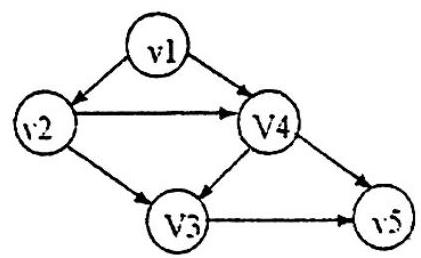
\includegraphics[width=0.3\textwidth]{images/2012/blanks_3.jpg}
\end{center}
\hspace*{3em} 

14. 若对序列(45,38,65,97,76,12,28,56)采用直接选择排序法排序,则第二趟结束后序列的状态是\_\_\_\_\_。

15. 高度为 4 的二叉平衡树最少有\_\_\_\_\_个结点。

16. 对于键值序列 \(\{ {11},{13},{10},{18},{50},{15},7,{20},{25},{90}\}\) ,建立初始堆,必须从键值为\_\_\_\_\_的结点开始对每个结点进行一次堆调整。

\section*{三、问答题(本大题共 6 小题,每小题 8 分,共 48 分)}

1. 在双循环链表中,写出在指针 \(\mathrm{p}\) 所指结点之后插入指针 \(\mathrm{s}\) 所指结点的执行语句序列。结点定义如下:

struct Node\{

\hspace*{1em} char data;

\hspace*{1em} Node *next;

\hspace*{1em} Node *prior;

\};

\vspace{5em}

2. 已知二叉树的先序序列和中序序列分别为 ABDGCEFH 和 DGBAECHF:

(1) 画出该二叉树;

(2)写出此二叉树的后序序列；

(3)画出与此二叉树对应的森林。
\vspace{5em}


\newpage
3. 已知由 12 个关键字构成的序列18、31、13、11、20、35、25、8、4、24、 40、27:

(1)请画出该序列的二叉排序树；

(2)给出删除结点 18 后的二叉排序树。
\vspace{5em}


4. 已知初始序列(50,80,63,45,48,92),写出直接插入排序的各趟排序的结果。
\vspace{5em}


\newpage
5. 设 Hash 函数为 \(\mathrm{H}\left( \mathrm{K}\right) = \mathrm{K}{\;\operatorname{mod}\;7}\) ,哈希表的地址空间为0,1,2,3,4,5,6, 开始时哈希表为空, 用二次探测再散列法解决冲突, 请画出依次插入键值 16 、 21、23、6、30、12、18 后的哈希表。
\vspace{8em}

6. 已知序列 45、15、20、35、25、60,请画出依次插入该序列的 AVL 树(平衡二叉树)。
\vspace{10em}

\section*{四、算法应用、分析题(本大题共 2 小题,第 1 小题 12 分,第 2 小题 8 分,共 20 分)}

1. 设一个无向网 \(G\) 如下:

\begin{center}
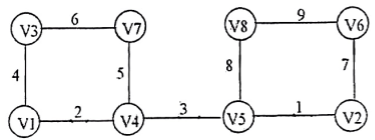
\includegraphics[width=0.6\textwidth]{images/2012/algorithm_1.png}
\end{center}


(1)请写出图 \(G\) 的邻接矩阵 \(A\) ；

(2)如果对某个顶点的邻接点的访问顺序按序号从小到大排列,请写出从顶点 \(\mathrm{v}1\) 出发,按“深度优先”和“广度优先”搜索方法遍历网 G 所得到的顶点序列: 

(3)从顶点 vl 出发,按照最小生成树的 Prim 算法,画出网 \(G\) 的一棵最小生成树。
\vspace{20em}

2. 已知某字符串 \(S\) 中共有 \(A\) 、 \(B\) 、 \(C\) 、 \(D\) 、 \(E\) 、 \(F\) 、 \(G\) 和 \(H\) 共 8 种字符,各种字符分别出现 2 次、1 次、4 次、5 次、7 次、3 次、4 次和 10 次,对该字符串用 \(\{ 0,1\}\) 进行前缀编码: 

(1)请画出对应的 Huffman 树,并给出各字符的前缀编码: 

(2)该字符串 \(S\) 的编码有多少位？
\vspace{20em}

\section*{五、算法设计题(本大题共 1 小题, 共 10 分)}

1. 有一个单链表 L (至少有一个结点),其头结点指针为 L,编写一个过程将 L 置逆,要求逆转在原链表上进行。单链表中的结点定义如下:

struct Node \{

\hspace*{1em} char data;

\hspace*{1em} Node *next;

\};

\newpage

\chapter{2013}

\section*{一、选择题(本大题共 20 小题,每小题 2 分,共 40 分)}

1. 计算机算法指的是解决问题的有限运算序列, 它必须具备输入、输出和 (   )等 5 个特性。

A. 可执行性、可移植性和可扩充性

B. 可行性、确定性和有穷性

C. 确定性、有穷性和稳定性

D. 易读性、稳定性和安全性

2. 某算法代码段如下,其时间复杂度是(   )。

% 为了让字体和图片中的更像，并设置为C语言风格
\begin{lstlisting}[language=C, basicstyle=\ttfamily]
for(i=1; i<=n; ++i)
  for(j=1; j<=n; ++j)
    {     c[i][j]=0;
          for(k=1; k<=n; ++k)
            c[i][j]+=a[i][k]*b[k][j];
    }
\end{lstlisting}

A. \(O\left( {n}^{2}\right)\) B \(O\left( {n}^{3}\right)\) C. \(O\left( n\right)\) D. \(O\left( {n{\log }_{2}n}\right)\)

3. 和顺序(连续)存储结构相比,线性表的链式存储结构的优点是(   )。

A. 所有操作/运算的算法都简单 . B. 便于随机存取

C 便于插入和删除 D. 便于查找

4. 在某线性表中最常用的操作是在最后一个元素之后插入一个元素和删除第一个元素,则采用(   )存储方式最节省运算时间。

A. 单链表 

B. 仅有头指针的单循环链表

C. 双向链表 

D. 仅有尾指针的单循环链表

5. 在线性表的下列运算中,不会改变数据元素之间结构关系的运算是(   )。

A. 插入 B. 删除 C. 排序 D. 查找

6. 在解决计算机主机与打印机之间速度不匹配问题时通常设置一个打印数据缓冲区,主机将要输出的数据依次写入该缓冲区,而打印机则依次从该缓冲区中取出数据打印。则该缓冲区作为数据结构是一个(   )结构。

A. 队列 B. 栈

C. 链表 D. 都不是

7. 栈和队列的共同点有(   )。

A. 都是先进先出 B. 都是后进先出

C. 不会删除中间的元素 D. 完全没有共同点

8. 设循环队列中数组的下标范围是 0.. \(\mathrm{n} - 1\) ,其头指针 front 指向队首元素, rear 指向队尾元素,则队列的长度为 (  )。

A. rear-front 

B. rear-front +1

C. \(\left( {\text{ rear } - \text{ front } + 1}\right) \% \left( {\mathrm{n} + 1}\right)\) 

D. (rear-front \(+ \mathrm{n} + 1\) ) \%n

9. 数组 \(\mathrm{A}\) 中,每个元素 \(\mathrm{A}\) 的长度为 3 个字节,行下标 \(\mathrm{i}\) 从 1 到 8 ,列下标 \(\mathrm{j}\) 从 1 到 10 ,从首地址 SA 开始连续存放在存储器内,该数组按行优先存放时, 元素 \(\mathrm{A}\left\lbrack  8\right\rbrack  \left\lbrack  5\right\rbrack\) 的起始地址为(   )。

A. SA+141 B. SA+222

C. SA+144 D. SA+225

10. 二叉树中(树根为第 1 层)第 5 层上的结点个数最多为(   )

A. 8 B. 15 C. 16 D. 32

11. 高度为 3 的二叉平衡树(空树高度为 0 )最少有(   )个结点。

A. 4 B. 15 C. 11 D. 7

12. 设高度为 \(\mathrm{h}\) (空树高度为 0 ) 的二叉树上只有度为 0 和度为 2 的结点,则此类二叉树中所包含的结点数至少为(   )。

A. \(2\mathrm{\;h}\) B. \(2\mathrm{h} - 1\) C. \(2\mathrm{h} + 1\) D. h+1

13. 将一棵有 100 个结点的完全二叉树从上到下 (根这一层), 每一层上从左到右依次对结点进行编号, 根结点的编号为 1 , 则编号为 49 的结点的左孩子编号为(   )。

A. 98 B. 48 C. 99 D. 50

14. 一棵哈夫曼树(Huffman Tree)的 4 个叶子结点的权值分别为 3, 9, 2, 7, 该树的带权路径长度为(   )。

A 38 B. 37 C. 44 D. 46

15. 图的邻接矩阵表示法适用于表示 (   )。

A. 无向图 B. 有向图 C. 稠密图 D. 稀疏图

16. 设图连通 G 采用邻接表存储,则深度优先遍历算法的时间复杂度是(   )。

A. O(n) B. O(n+e) C. \(O\left( {n}^{2}\right)\) D. \(\mathrm{O}\left( {{\mathrm{n}}^{4}\mathrm{e}}\right)\)

17. 顺序查找算法在查找成功情况下的平均比较次数是(   )。

A. \({\mathrm{n}}\) B. \({\mathrm{n}}^{2}\) C. \(\log \left( \mathrm{n}\right)\) D \(\left( {n + 1}\right) /2\)

18. 散列 (哈希, Hash) 函数有一个共同性质, 即其函数取值在值域里呈现(   )。

A. 均匀分布 B. 正态分布 C. 泊松分布 D. 任意分布

19. 时间复杂度不受待排序序列初始状态的影响,总是 \(O\left( {n}^{2}\right)\) 的是(   )。

A. 直接插入排序 B. 快速排序 C. 简单选择排序 D. 归并排序


20. 以比较为基础的排序算法在最坏情况下的计算时间复杂度下界为(   )

A. \(O\left( {n}^{2}\right)\) B. \(O\left( {{\log }_{2}n}\right)\) C. \(O\left( n\right)\) D. \(O\left( {n{\log }_{2}n}\right)\)

\section*{二、填空题(本大题共 17 小题,每小题 2 分,共 34 分)}

1. 求整数 \(\mathrm{n}\left( {\mathrm{n} \geq  0}\right)\) 阶乘函数的递归算法如下,其时间复杂度是(   )

\begin{lstlisting}[language=C, basicstyle=\ttfamily]
long Factorial(long n) {
    if(n == 0) return 1;
    else return n*Factorial(n-1);
}
\end{lstlisting}

2. 某算法中的语句频度之和为 \(T\left( n\right)  = 2{n}^{2} + {5n} + 2\) ,则其时间复杂度为 (   )。

3. 已知栈的输入序列为 1,2,3,4,5,6,7输出序列为 a1, a2, a3, a4, a5, a6, a7 符合 a2 =7 条件的输出序列共有(   )个。

4. 采用特殊字符作为结尾的顺序存储方式存储,则串 “MyDataS” 最少需要 (   )个字符的存储空间。

5. 已知某二叉树的先序序列 ABCDEGF, 中序序列 CBEGDFA, 那么它的后序遍历序列是 (   )

6. 已知完全二叉树的第 4 层(根结点为第 1 层)总共只有 3 个结点,则其叶子结点数是(   )。

7. 某表达式二叉树按后序遍历的结果为 abcd-*+ef/-,令 \(a = 2,b = 3,c = 4,d = 5\) , \(e = 6,f = 2\) ,则该表达式的值等于(   )。

8. 在一棵度为 3 的树中, 度为 2 的结点个数是 1 , 度为 0 的结点个数是 6 , 则度为 3 的结点个数是(   )。

9. 高度为 \(\mathrm{k}\) (空树高度为 0 )的完全二叉树至少有(   )个结点。

10. 含 \(\mathrm{n}\) 个顶点的无向连通图中至少含有(   )条边。

11. 在具有 20 个元素的顺序表 (查找表) 上进行折半查找 (二分查找), 需比较五次并查找成功的元素个数是(   )

12. 判别下面的序列是否为堆(若是, 明确小根堆或大根堆)? (100,86,48,73,35,39,42,57,66,21);

13. 应用 Dijkstra's 算法(单源最短路径)求图 1 顶点 v6 到其他顶点的最短路径,最先求出的是顶点 \(\mathrm{v}6\) 到顶点(   )的最短路径。

14. 有 8 个球队参加的某联赛按单循环方式进行比赛,其需要进行的比赛场次为(   ), 和完全无向图的边数一样多。

15. 由 6 个权值构造的哈夫曼树(Huffman Tree)有(   )个结点。

16. 在非空 m 阶 B 树上。除根结点以外的所有其他内部结点含有(   )棵子树。

17. 给出图 2 的一个拓扑序列(   )。

% \begin{center}
% 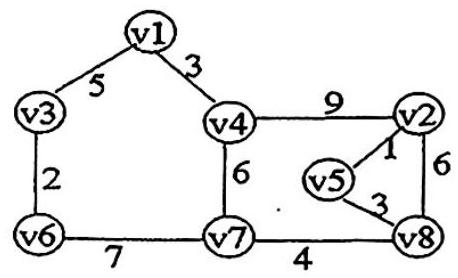
\includegraphics[width=0.3\textwidth]{images/2013/blank_17_1.jpg}
% 图 1
% \end{center}
% \hspace*{3em} 

\begin{figure}[htbp]
    \centering
    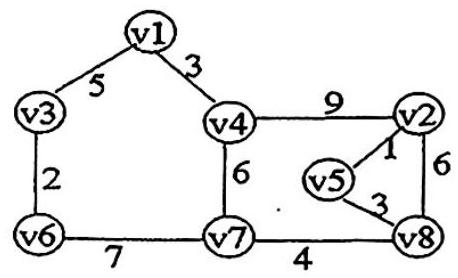
\includegraphics[width=0.3\textwidth]{images/2013/blank_17_1.jpg}
    \caption*{图1} % 使用带星号的 caption*
\end{figure}

\begin{figure}[htbp]
    \centering
    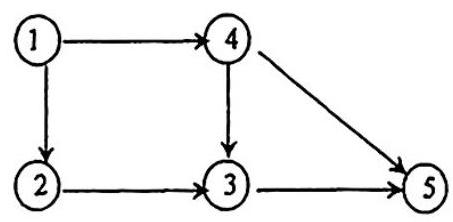
\includegraphics[width=0.3\textwidth]{images/2013/blank_17_2.jpg}
    \caption*{图2} % 使用带星号的 caption*
\end{figure}

\section*{三、问答题(本大题共 7 小题,每小题 8 分,共 56 分)}

1. 在一个长度为 \(\mathrm{n}\) 的单链表 \(\mathrm{L}\) 中,现需删除链表中 \(* \mathrm{p}\) 结点的前驱结点,试简要说明该操作的实现思想, 并分析时间复杂度。
\vspace{5em}

2. 具有 8 个结点的某森林的孩子一兄弟存储结构刚好构成完全二叉树。请画出原来的森林的结构。
\vspace{10em}

\newpage
3. 现有无向图如图 3 所示,从顶点 \(\mathrm{F}\) 开始使用 Prim(普里姆) 算法求图的最小生成树, 要求必须清楚地表明其生成过程。
\vspace{7em}

4. 现有无向图如图 3 所示, 完成下面任务: 

(1)画出图的邻接矩阵图示; 

(2)从顶点 \(\mathrm{H}\) 开始对图进行广度优先遍历,写出遍历结果。
\vspace{10em}

\newpage
5. 已知一棵二叉排序树结构如图 4 所示, 各结点的数据从小到大依次为 15,25,37,49,51,66,请重建出完整的原二叉树。
\vspace{10em}

6. 设 Hash 函数为 \(\mathrm{H}\left( \mathrm{{key}}\right)  = \mathrm{{key}}{\;\operatorname{mod}\;7}\) ,哈希表的地址空间为 \(0,1,\ldots ,{10}\) ,开始时哈希表为空, 用平方探测法解决冲突。回答下列问题:

1)请画出依次插入键值9,14,10,30,56后的哈希表？

2) 对表中关键字 14,30 和 56 进行查找时,所需进行的比较次数各为多少?
\vspace{10em}

\newpage
7. 对关键字序列(51,32,66,92,75,16,25,46)按从小到大进行快速排序。 设选第一个元素为支点/参考值 (pivot),写出排序过程中第 1 趟的划分结果；

\begin{figure}[htbp]
    \centering
    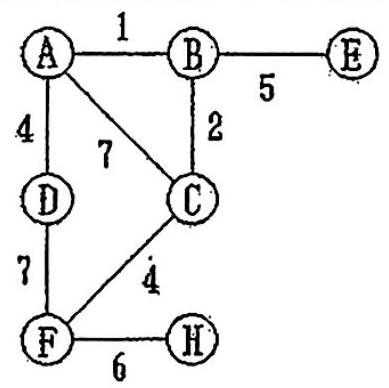
\includegraphics[width=0.3\textwidth]{images/2013/ask_7_1.jpg}
    \caption*{图3} % 使用带星号的 caption*
\end{figure}

\begin{figure}[htbp]
    \centering
    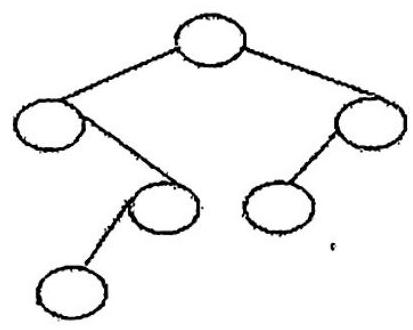
\includegraphics[width=0.3\textwidth]{images/2013/ask_7_2.jpg}
    \caption*{图4} % 使用带星号的 caption*
\end{figure}

\vspace{10em}

\section*{四、算法设计、分析题(本大题共 2 小题,每小题 10 分,共 20 分)}

1. 现有一棵二叉查找 (排序) 树 (Binary Search Tree) BST, 以二叉链表形式存储, 进行中序遍历可得到从小到大排列的有序序列。试设计一算法, 对该二叉查找树进行变换, 使得对新的二叉树进行中序遍历可得到从大到小排列的有序序列。要求:

(1)描述算法的基本设计思想。

(2)根据设计思想,描述算法的详细实现步骤 ,可使用伪代码、C或C++或 JAVA 语言,关键之处给出简要注释。

有关的数据结构已描述如下:

\begin{lstlisting}[language=C, basicstyle=\ttfamily]
struct Binary_node {
    int data;
    Binary_node *left;
    Binary_node *right;
}
\end{lstlisting}
\vspace{10em}

2. 某顺序表中的数据序列为降序序列, 试设计一算法将数据序列变换为升序序列。要求:

(1)描述算法的基本设计思想。

(2)根据设计思想,描述算法的详细实现步骤,可使用伪代码、C 或 C++或 JAVA 语言,关键之处给出简要注释。

(3)分析算法时间复杂度、空间复杂度。
\newpage

\chapter{2014}
\section*{一、选择题(本大题共 20 小题,每小题 2 分,共 40 分)}

1. 下面程序段的时间复杂度是 (  )。
\begin{lstlisting}[language=C, basicstyle=\ttfamily]
for i=0;i<m;i++)
    A[i]=0;
for(i=0;i<m;i++)
    for (j=1;j<n;j++)
        A[i]+=5;
\end{lstlisting}

A \(\mathrm{O}\left( {\mathrm{m} + \mathrm{n}}\right)\) B \(\mathrm{O}\left( {\mathrm{m} + \mathrm{n} + 1}\right)\) C O(n) D \(\mathrm{O}\left( {{\mathrm{m}}^{ * }\mathrm{n}}\right)\)

2. 计算机算法指的是 (  ), 它必须具备输入、输出和可行性、确定性和有穷性等 5 个特性。。

A 计算方法 B 排序方法

C 解决问题的有限指令序列 D 调度方法

3. 若某栈的输入序列为 1,2,3,..., n,输出序列的第 2 个元素为 n,则第 3 个输出元素为 (  )。

A 1 或 2 B 1 或 \(\mathrm{n} - 1\) C \(\mathrm{n} - 1\) 或 \(\mathrm{n} - 2\) D \(\mathrm{n} - 1\)

4. 线性表的链式存储结构与顺序(连续)存储结构相比优点是(  )。

A. 便于插入和删除 B. 便于随机存取

C. 所有的操作/运算的算法简单 D. 便于查找

5. 设循环队列中数组的下标范围是 \(0..\mathrm{n} - 1\) ,其头指针 front 指向队首元素, rear 指向队尾元素,则队列的长度为(  )。

A rear-front B rear-front + 1

C (rear-front +1) \% (n+1)

D (rear-front \(+ \mathrm{n} + 1\) ) \%n

6. 如果某应用在线性表中最常用的操作是在最后一个元素之后插入一个元素和删除第一个元素, 则采用 (  ) 存储方式最节省运算时间。

A. 仅有头指针的单链表 B. 仅有头指针的单循环链表

C. 双链表 D. 仅有尾指针的单循环链表

7. 在长度为 \(\mathrm{n}\) 且带头结点的链式存储实现的线性表的第 \(\mathrm{i}\left( {0 \leq  \mathrm{i} \leq  \mathrm{n}}\right)\) 个位置插入一个元素, 需要查找运算( )次。

A. 1 B. n-i C. i D. n-2

8. 在长度为 \(\mathrm{n}\) 顺序实现的线性表的第 \(\mathrm{i}\left( {1 \leq  \mathrm{i} \leq  \mathrm{n}}\right)\) 个位置之前插入一个元素,需要后移 \(\left( \right)\) 个元素。

A. i B. n-i+1 C. n D. 1

9. 数组 A 中,每个元素 A 的长度为 4 个字节,行下标 i 从 1 到 8 ,列下标 j 从 1 到 10 , 从首地址 \(\mathrm{S}\) 开始连续存放在存储器内,该数组按行优先存放时,元素 \(\mathrm{A}\left\lbrack  5\right\rbrack  \left\lbrack  6\right\rbrack\) 的起始地址为(  )。

A. S+160 B. S+180 C. S+220 D. S+140

10. 设高度为 \(\mathrm{h}\) 的二叉树上只有度为 0 和度为 2 的结点,则此类二叉树中所包含的结点数至少为(  )。

A. \(2\mathrm{\;h} - 1\) B. \(2\mathrm{\;h}\) C. \(2\mathrm{\;h} + 1\) D.h+1

11. 已知完全二叉树有 10 个结点, 则整棵二叉树有 (  ) 个度为 1 的结点

A. 2 B. 1 C. 0 D. 不确定

12. 在所有排序方法中,关键字比较的次数与记录的初始排列次序无关的是(  ).

A. 直接插入排序 B. 希尔(Shell)排序

C. 简单选择排序 D 冒泡排序

13. 在常用的哈希表处理冲突的方法中,(  )方法容易产生 “二次聚集”,导致哈希表性能变差。

A. 开放定址法一线性探测 B. 再哈希法 C. 链地址法

E. 开放定址法一二次探测

14. 对包含 \(n\) 个元素的散列表进行查找,平均查找长度 (  )

A. 为 \(O\left( {{\log }_{2}n}\right)\) B. 为 \(O\left( n\right)\) C. 不直接依赖于 \(n\) D. \(O\left( {n{\log }_{2}n}\right)\)

15. 对一棵二叉排序 (升序、查找) 树的根结点而言, 左子树中所有结点的关键字都 (  ) 右子树中所有结点的关键字。

A. 不等于 B. 不大于 C. 等于 D. 大于

16. 在对 \(\mathrm{n}\) 个关键字进行简单选择排序的过程中,每一趟都要从无序区选出最小关键字元素,则在进行第 \(\mathrm{i}\) 趟排序之前,无序区中关键字元素的个数为 (  )

A. i B. \(\mathrm{i} + 1\) C. n-i D. n-i+1

17. 下面的关键码序列中哪一个是堆( ？ )。

A.18,72,35,23,94,53 B.18,31,23,94,53,72

C.18,53,23,94,40,72 D.94,55,18,72,16,23

18. 设连通图 G 采用邻接表存储,则深度优先遍历算法的时间复杂度是(  )。

A.O(n) B.O(n+e) C. \(O\left( {n}^{2}\right)\) D.O(n*e)

注: 所有答案必须写在答题纸上, 试卷上作答无效 !

19. 已给右图,(  )是该图的拓扑排序？

A.1,2,3,4,5

\begin{center}
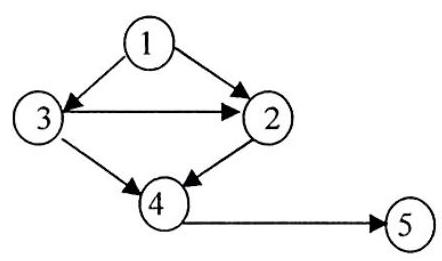
\includegraphics[width=0.3\textwidth]{images/2014/choice_19.jpg}
\end{center}
\hspace*{3em} 

B.1,2,4,3,5

C.1,3,2,4,5

D.1,2,3,5,4

20. 图的邻接矩阵表示法适用于表示 (  )

A. 稠密图 B. 有向图 C. 无向图 D. 稀疏图

\section*{二、填空题(本大题共 17 小题,每小题 2 分,共 34 分)}

1. 设一循环队列 \(\mathrm{Q}\) 中, rear 指针指向队尾元素的下一个位置, front 指针指向队首元素, 则判断队列中元素为空的条件是\_\_\_\_\_\_\_\_。

2. 设栈 \(\mathrm{S}\) 和队列 \(\mathrm{Q}\) 的初始状态皆为空,元素 \(\mathrm{a}1,\mathrm{a}2,\mathrm{a}3,\mathrm{a}4,\mathrm{a}5,\mathrm{a}6\) 和 \(\mathrm{a}7\) 依次通过一个栈,一个元素出栈后即进入队列 \(\mathrm{Q}\) ,若 7 个元素出队列的顺序是 \(\mathrm{a}3,\mathrm{\;a}5,\mathrm{\;a}4,\mathrm{\;a}7,\mathrm{\;a}6\) , a2, a1 则栈 S 至少应该容纳\_\_\_\_\_\_\_\_个元素。

3. 广义表 L \(= \left( {{\left( a\right) }_{3}\left( {b,c}\right) ,\left( d\right) }\right) ,L\) 的长度是\_\_\_\_\_\_\_\_。

4. 二叉树中第 5 层上(根在第 1 层)的结点个数最多为\_\_\_\_\_\_\_\_。

5. 某算法中的语句频度之和为 \(T\left( n\right)  = 3{n}^{2} + {2n} + 7\) ,则其时间复杂度为\_\_\_\_\_\_\_\_。

6. 某表达式语法树(二叉树)按后序遍历的结果为 abc-d+*h-,令 a=2, b=6, c=4, d=5, h=8,则该表达式的值等于\_\_\_\_\_\_\_\_。

7. 采用特殊字符作为结尾的顺序存储方式存储,若两个串的长度分别为 \(\mathrm{m}\) 和 \(\mathrm{n}\) ,则两个串相等与否的比较运算的时间复杂度为\_\_\_\_\_\_\_\_。

8. n 阶矩阵中三角矩阵使用压缩存储方式时需要\_\_\_\_\_\_\_\_个数据元素空间来存储。

9. 一棵含有 20 个结点的二叉树的高度至少为\_\_\_\_\_\_\_\_(空树高度为 0)。

10. 已知某二叉树的先序序列 ABCFDG, 中序序列 CBDFAG, 那么它的后序遍历序列是\_\_\_\_\_\_\_\_。

11. 含 \(\mathrm{n}\) 个顶点的无向连通图中至少含有\_\_\_\_\_\_\_\_条边。

12. 采用特殊字符作为结尾的顺序存储方式存储, 则串 “GLuckyUProgram” 至少\_\_\_\_\_需要个字符的存储空间。

13. 请指出在顺序表 \(\{ 3\text{ 、 }6\text{ 、 }8\text{ 、 }{10}\text{ 、 }{14}\text{ 、 }{15}\text{ 、 }{18}\text{ 、 }{36}\text{ 、 }{44}\text{ 、 }{62}\}\) 中,用二分法/折半法查找关键码 10 需做\_\_\_\_\_\_\_\_次关键码比较。

14. 高度为 5 的 AVL 树(平衡二叉树)至少有\_\_\_\_\_\_\_\_个结点。(空树高度为 0)

15. 应用 Dijkstra's 算法(单源最短路径)求下图顶点 \(\mathrm{A}\) 到顶点 \(\mathrm{D}\) 的最短路径,第 1 步、第 2 ”步求出的是顶点 \(\mathrm{A}\) 到顶点\_\_\_\_\_\_\_\_, \({\mathrm{A}}^{\prime }\) 到顶点\_\_\_\_\_\_\_\_的最短路径。

\begin{center}
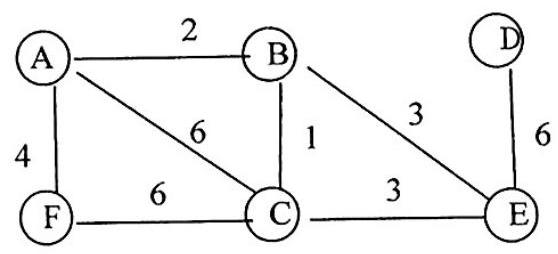
\includegraphics[width=0.4\textwidth]{images/2014/blank_15.jpg}
\end{center}
\hspace*{3em} 

16. 对于键值序列 \(\{ {16},{85},{28},{58},{17},5,{18},{25},{81},{32},{98}\}\) ,建里初始堆,必须从键值为\_\_\_\_\_\_\_\_ 的结点开始对前面的每个结点进行一次堆调整。

17. 排序过程中,对尚未确定最终位置的所有数据元素进行一遍处理称为一趟排序,下列五种排序方法中,每一趟排序结束时都至少能够确定一个元素最终位置的方法有\_\_\_\_\_\_\_\_

I. 简单选择排序 (Shell) 排序 III. 快速排序

IV. 维排序 V. 两路归并排序

\section*{三、问答题(本大题共 8 小题,每小题 7 分,共 56 分)}

1. 在顺序表中插入一个结点需平均移动多少个结点 分析此操作的时间复杂度。

2. 设下图为某树的二叉树表示, 请画出该树。

\begin{center}
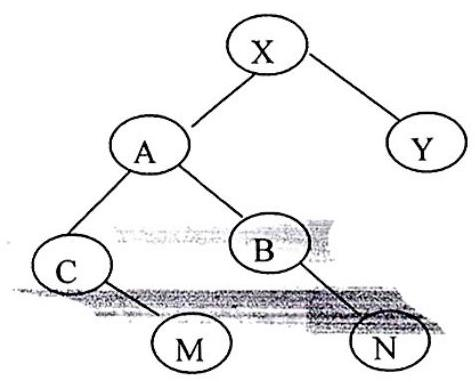
\includegraphics[width=0.4\textwidth]{images/2014/ask_2.jpg}
\end{center}
\hspace*{3em} 
\vspace{5em}

\newpage
3. 已知关键字序列为45,32,22,37,70,42,依次将各元素插入到一棵初始为空的二叉排序树, 画出对应的二叉排序树。
\vspace{10em}

4. 简要说明快速排序的排序思想, 并给出算法时间复杂度。根据所给序列 (50,25,35,80,90,15,99,68),设选第一个元素为支点/参考值 (pivot), 采用双向交替向中间扫描的方式, 写出快速排序的第一趟排序的结果。
\vspace{10em}

\newpage
5. 下图有六个顶点 A、B、C、D、E、F,其连接关系及相应权值如图所示。 给出邻接矩阵表示结果, 然后从顶点 \(\mathrm{A}\) 开始对图进行广度优先遍历, 写出遍历结果。

\begin{center}
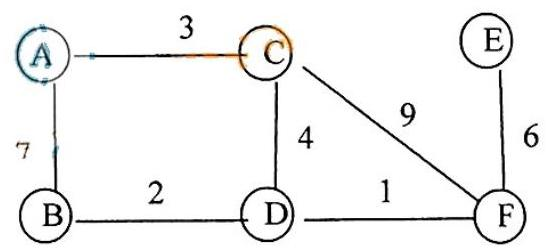
\includegraphics[width=0.4\textwidth]{images/2014/ask_5.jpg}
\end{center}
\hspace*{3em} 
\vspace{12em}

6. 使用 Kruskal 算法求第 5 题所给图 (上图) 的最小生成树, 必须给出树的生成过程。
\vspace{15em}

\newpage
7. 已给输入关键字序列 \(\{ {23},{12},{17},{60},{30},{36},{40},{42}\}\) ,哈希函数为 \(\mathrm{H}\) (key) = key \%9, 哈希表的地址空间为 0, 1, ..., 8, 开始时哈希表为空, 用线性探测法解决冲突, 请依次画出插入键值后的 Hash (哈希) 表, 出现冲突时单独标示清楚。
\vspace{12em}

8. 假设用于通信的电文由字符集 \(\{ X,Y,C,D,F\}\) 中的字母构成,这 5 个字母在电文中出现的频率依次为 \(\{ {35},{20},{10},{13},{22}\}\) 。请画出对应的编码哈夫曼树 (Huffman)。
\vspace{15em}

\section*{四、算法设计、分析题(本大题共 2 小题, 每小题 10 分, 共 20 分)}

1. 现有二叉平衡树(或为空树,或者根结点的左右子树高度差最大为 1 且左、 右子树为二叉平衡树), 试设计一算法判断该二叉树是否为二叉平衡树。

1)先给出设计思想；

2)再描述具体算法, 必要时请给予注释说明。
\vspace{15em}
\vspace{15em}

2. 现有某比赛活动中某选手的 \(\mathrm{n}\) 个评分结果 (百分制,已知都在 60 以上的整数)已存入顺序表中,并且已按升序排序。为了分析相关规律, 现需分析评分的 k -均值直方图(以当前分数为中位数(位置在中间),计算最邻近的 k 个分数平均值并取为整数, 然后统计分数的频率得到。若当前分左边或右边数据不足时直接忽略, 不计入统计数据), 请设计一尽量快速的算法, 求得打印直方图前的统计结果。

1)先给出设计思想；

2)再描述具体算法, 必要时请给予注释说明。

\newpage

\chapter{2015}
\section*{一、 选择题(本大题共 20 小题,每小题 2 分,共 40 分)}

1. 下面程序段的时间复杂度为(   )。

\begin{lstlisting}[language=C, basicstyle=\ttfamily]
m=10,n=10;s=0;
for (i=0;i<m;i++)
    for (j=0;j<n;j++)
        s+=i*j;
\end{lstlisting}

A. \(O\left( {m}^{2}\right)\) B. \(O\left( {n}^{2}\right)\)

C. \(O\left( {{m}^{ * }n}\right)\) D. \(O\left( 1\right)\)

2. 在线性表的下列运算中,不改变数据元素之间结构关系的运算是(   )。

A. 插入 B. 删除

C. 排序 D. 查找

3. 线性表采用链表存储时地址(   )。

A. 必须是连续的 B. 部分地址必须是连续的

C. 一定是不连续的 D. 连续不连续都可以

4. 在解决计算机主机与打印机之间速度不匹配问题时通常设置一个打印数据缓冲区,主机将要输出的数据依次写入该缓冲区,而打印机则依相同次序从该缓冲区中取出数据打

印。该缓冲区作为数据结构是一个(   )结构。

A. 栈 B. 队列 C. 哈希表 (Hash Table) D. 线性表

5. 一个栈的输入序列为 1, 2, 3, 4,下面哪一个序列不可能是这个栈的输出序列(   )？

A.2,3,4,1 B.4,3,1,2

C.1,3,2,4 D.3,4,2,1

6. 设计一个判别表达式中左、右括号是否配对出现的算法, 采用 (   ) 数据结构最佳。

A. 栈 B. 队列 C. 顺序结构线性表 D. 链式结构线性表

注:所有答案必须写在答题纸上,试卷上作答无效！

7. 在长度为 \(\mathrm{n}\) 顺序实现的线性表的第 \(\mathrm{i}\left( {1 \leq  \mathrm{i} \leq  \mathrm{n}}\right)\) 个位置之前插入一个元素,需要后移 (   )个元素。

A. 0 B. i C. 1 D. n-i+1 (10.3.15)

8. 链表不具有的特点是(   )。

A. 可随机访问任一元素 B. 插入、删除不需要移动元素

C. 不必事先估计存储空间 D. 所需空间与线性表长度成正比

9. 将一个 \(\mathrm{A}\left\lbrack  {20}\right\rbrack  \left\lbrack  {20}\right\rbrack\) (下标从 1 开始计算)的矩阵按行优先顺序存放,每个元素占 4 个存储单元,并且 \(\mathrm{A}\left\lbrack  1\right\rbrack  \left\lbrack  2\right\rbrack\) 的存储地址是 1004,则 \(\mathrm{A}\left\lbrack  {20}\right\rbrack  \left\lbrack  2\right\rbrack\) 的地址是(   )。

A. 1004 B. 1380 C. 1520 D. 2524

10. 树根的层数为 1 ,则一棵含 12 个结点的二叉树的高度至多为(   )。

A. 3 B. 4 C. 11 D. 12

11. 已知二叉树如下图,下列序列中,(   )是后序遍历后得到的序列。

\begin{center}
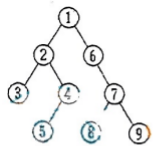
\includegraphics[width=0.2\textwidth]{images/2015/choice_11.png}
\hspace*{3em} 
\end{center}

\begin{tabular}{lccccccccc}
\text{A.3} & 5 & 4 & 2 & 8 & 9 & 7 & 6 & 1 \\
\text{B.3} & 4 & 5 & 2 & 8 & 9 & 7 & 6 & 1 \\
\text{C.1} & 2 & 3 & 4 & 5 & 6 & 7 & 8 & 9 \\
\text{D.2} & 3 & 4 & 5 & 6 & 7 & 8 & 9 & 1 \\
\end{tabular}

12. 已知数据表 A 中每个元素距其最终位置不远,则采用(   )排序算法最节省时间。

A. 堆排序 B. 直接插入排序 C. 快速排序 D. 简单选择排序

13. 请指出在顺序表 \(\{ 2\) 、5、7、10、14、15、18、23、35、41、 \({52}\}\) 中,用二分法查找关键码 12 需做多少次关键码比较(   )。

A. 2 B. 3 C. 5 D. 4

14. 查找 Hash 表,不会发生冲突的哈希函数是(   )。

A. 除留余数法 B. 伪随机探测再散列

C. 直接地址法 D. 线性探测再散列法

15. 对包含 N 个元素的散列表进行查找,平均查找长度(   )。

A、为 \(\mathrm{O}\left( {{\log }_{2}\mathrm{N}}\right)\) B、为 \(\mathrm{O}\left( \mathrm{N}\right)\) C、不直接依赖于 \(\mathrm{N}\) D、上述三者都不是

16. 下面四棵树中,数字表示相应叶子结点的权值,则(   )是哈夫曼树。 

A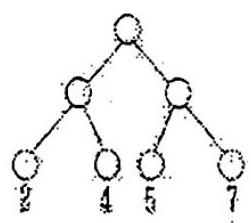
\includegraphics[width=0.2\textwidth]{images/2015/choice_16_A.jpg}
B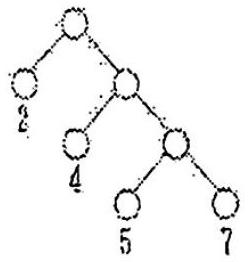
\includegraphics[width=0.2\textwidth]{images/2015/choice_16_B.jpg}
C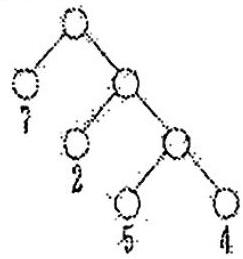
\includegraphics[width=0.2\textwidth]{images/2015/choice_16_C.jpg}
D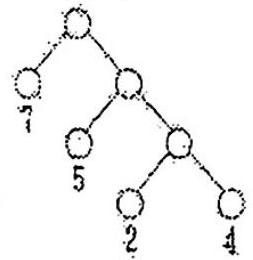
\includegraphics[width=0.2\textwidth]{images/2015/choice_16_D.jpg}

17. 下列排序算法中,(   )算法可能会出现下面情况:初始数据有序时,花费时间反而最多。 

A. 堆排序 B. 冒泡排序 C. 快速排序 D. 直接插入排序

18. 给定下列有向图和初始结点 V1,按深度优先遍历的结点序列为(   )。

\begin{center}
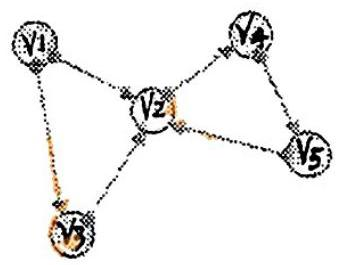
\includegraphics[width=0.2\textwidth]{images/2015/choice_18.jpg}
\end{center}
\hspace*{3em} 

A、V1, V3, V4, V5, V2

B、V1, V2, V3, V4, V5

C、V1, V2, V5, V3, V4

D、V1, V2, V4, V5, V3

19. 下面关于图的存储的叙述中, 哪一个是正确的(   )。

A. 用邻接矩阵法存储图,占用的存储空间数只与图中结点个数有关,而与边数无关。

B. 用邻接矩阵法存储图,占用的存储空间数只与图中边数有关,而与结点个数无关。

C. 用邻接表法存储图,占用的存储空间数只与图中结点个数有关,而与边数无关。

D. 用邻接表法存储图,占用的存储空间数只与图中边数有关,而与结点个数无关。

20. 在有向图的邻接表存储结构中,顶点 \(\mathrm{v}\) 在表结点中出现的次数等于(   )。

A. 顶点 \(\mathrm{v}\) 的度 B. 顶点 \(\mathrm{v}\) 的出度

C. 顶点 \(\mathrm{v}\) 的入度 D. 依附于顶点 \(\mathrm{v}\) 的边数

\section*{二、填空题(本大题共 17 小题,每小题 2 分,共 34 分)}

1. 设有一空队列 \(Q\) ,经 \(Q.{EnQueue}\left( 1\right) ,Q.{DeQueue}\left( \right) ,Q.{EnQueue}\left( 2\right) ,Q.{EnQueue}\left( 3\right) ,\) Q. EnQueue(4), Q. DeQueue (   ); Q. EnQueue (5)一系列操作后。队列中从队首到队尾的元素依次是\_\_\_\_\_。

2. 设栈 \(S\) 和队列 \(Q\) 的初始状态为空,元素 \(a\) 、 \(b\) 、 \(c\) 、 \(d\) 、 \(e\) 、 \(f\) 将依次入栈 \(S\) ,一个元素出栈后即进入队列 \(\mathrm{Q}\) 。若这 6 个元素出队列的顺序是 \(\mathrm{b}\text{ 、 }\mathrm{d}\text{ 、 }\mathrm{c}\text{ 、 }\mathrm{f}\text{ 、 }\mathrm{e}\text{ 、 }\mathrm{a}\) ,则栈 \(\mathrm{S}\) 的容量至少应该是\_\_\_\_\_,上述过程才不会错。

3. 已知完全二叉树的第 6 层(根结点为第 1 层)总共只有 5 个结点,则其叶子结点数是\_\_\_\_\_。

4. 用顺序存储的方法将完全二叉树中的所有结点逐层存放在数组 \(R\left\lbrack  {0,..,n - 1}\right\rbrack\) (下标从 0 开始计)中,结点 \(\mathrm{R}\left\lbrack  \mathrm{i}\right\rbrack\) 若有右子女,则右子女结点的下标是\_\_\_\_\_。

5. 某表达式二叉树按先序遍历的结果为 \(+ {\mathrm{a}}^{ * } + \mathrm{{bcd}}\) ,令 \(\mathrm{a} = 6,\mathrm{\;b} = 3,\mathrm{c} = 4,\mathrm{\;d} = 2\) ,则该表达式的值等于\_\_\_\_\_。

6. n 个元素的线性表,采用顺序存储结构,插入一个元素要平均移动表中\_\_\_\_\_个元素(假定在线性表任何位置上插入元素都是等概率的)。

7. 在一棵二叉树中, 度为 2 的结点有 50 个, 度为 1 的结点有 20 个, 该二叉树共有\_\_\_\_\_条边。

8. 含 12 个结点的平衡二叉树的最大深度是\_\_\_\_\_(设根节点的深度是 1)。

9. 设二叉树 \(\mathrm{T}\) 的前序遍历序列和中序遍历序列分别是: \(\mathrm{b},\mathrm{d},\mathrm{c},\mathrm{a},\mathrm{e},\mathrm{f}\) 和 \(\mathrm{c},\mathrm{d},\mathrm{e},\mathrm{a},\mathrm{b},\mathrm{f}\) ,则其后序遍历序列为\_\_\_\_\_。

10.6 阶 B-树 (B-Tree) 中, 每个结点至多包含 5 个关键码, 除根和叶结点外, 每个结点至少包含\_\_\_\_\_个关键码。

11. 具有 n 个叶子结点的哈夫曼树中,其结点总数为\_\_\_\_\_个。

12. G 为无向图,如果从 \(G\) 的某个顶点出发进行一次遍历,即可访问图的每个顶点,则该图一定是\_\_\_\_\_图。

13. 在一个图中,所有顶点的度数之和等于图的边数的\_\_\_\_\_倍。

14. 已知一个无向图的邻接矩阵表示,计算第 j 个结点的度的方法是\_\_\_\_\_。

15. 两个不同的关键字, 其哈希函数值相同, 因而被映射到同一表位置上, 这种现象称为\_\_\_\_\_。

\vspace{14em}

注:所有答案必须写在答题纸上,试卷上作答无效！ 第 5 页(共 9 页)

16. 对长度为 \(\mathrm{n}\) 的关键字序列进行快速排序的时间复杂度为\_\_\_\_\_。

17. 对于键值序列 \(\{ {12},{13},{11},{18},{60},{15},7,{18},{25},{100}\}\) 里建初始堆,必须从键值为\_\_\_\_\_的结点开始对每个结点进行一次堆调整。

\section*{三、问答题(本大题共 8 小题,每小题 7 分,共 56 分)}

1. 现有 2 棵树的森林如下图所示,请画出对应的二叉树。

\begin{center}
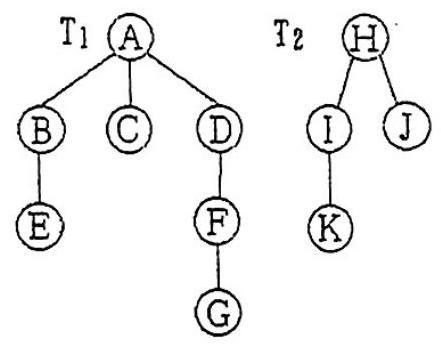
\includegraphics[width=0.3\textwidth]{images/2015/ask_1.jpg}
\end{center}
\hspace*{3em} 
\vspace{8em}

2. 已知关键字序列为36,31,20,32,66,48,依次将各元素插入到一棵初始为空的二叉排序树, 画出对应的二叉排序树。
\vspace{8em}

\newpage
3. 假设用于通信的电文由字符集 \(\{ \mathrm{A},\mathrm{B},\mathrm{C},\mathrm{D},\mathrm{E},\mathrm{F},\mathrm{G}\}\) 中的字母构成,这 7 个字母在电文中出现的频率依次为 \(\{ 3,{12},7,4,2,8,{11}\}\) 。请画出对应的编码哈夫曼树(Huffman)；求出每个字符的哈夫曼编码(约定编码时左分支编码 “0”,右分支编码为“1”。生成哈夫曼时, 同一层节点按左大右小排列)。
\vspace{8em}

4. 简要说明快速排序的排序思想。根据所给序列(49,38,65,97,76,13,27,50), 设选第一个元素为支点/参考值(pivot),写出快速排序的第一趟排序的结果。
\vspace{8em}

\newpage
5. 图 G 各顶点的连接关系及相应权值如下图所示。(1)画出该图的邻接距阵；(2)从顶点 V1 开始对图进行广度优先遍历,写出遍历结果(3)使用 Kruskal 算法求该图的最小生成树,画出其生成过程。

\begin{center}
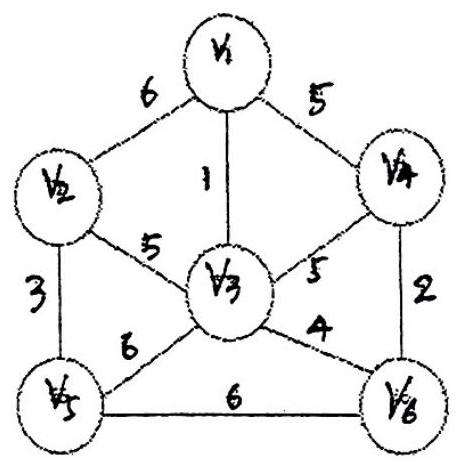
\includegraphics[width=0.3\textwidth]{images/2015/ask_5.jpg}
\end{center}
\hspace*{3em} 
\vspace{10em}

6. 以关键字序列(265,301,751,129,937,863,742,694,076,438)为例,分别写出执行以下排序算法的各趟排序状态和排序结束时关键字序列的状态。

(1)直接插入排序 

(2)希尔排序,增量序列为 5,3,1。上述方法中,哪些是稳定的排序？ 哪些是非稳定的排序?
\vspace{10em}

\newpage
7. 已知一组Key: (19 14 23 01 68 20 84 27 55 11 10 79), 按H(key) = key MOD 13 和 线性探测再散列 \(\mathrm{{Hi}} = \left( {\mathrm{H}\left( \mathrm{{key}}\right)  + \mathrm{{di}}}\right) \mathrm{{MOD}}\) 13 方法处理冲突,请画出最后得到的哈希表并填写相应的探测次数(完整下列表格即可)。

答: 哈希表如下:

\begin{center}
\begin{tabular}{|c|c|c|c|c|c|c|c|c|c|c|c|c|c|}
\hline
\phantom{X} & 0 & 1 & 2 & 3 & 4 & 5 & 6 & 7 & 8 & 9 & 10 & 11 & 12 \\
\cline{1-14}
哈希表 & \phantom{X} & \phantom{X} & \phantom{X} & \phantom{X} & \phantom{X} & \phantom{X} & \phantom{X} & \phantom{X} & \phantom{X} & \phantom{X} & \phantom{X} & \phantom{X} & \phantom{X} \\
\cline{1-14}
探测次数 & \phantom{X} & \phantom{X} & \phantom{X} & \phantom{X} & \phantom{X} & \phantom{X} & \phantom{X} & \phantom{X} & \phantom{X} & \phantom{X} & \phantom{X} & \phantom{X} & \phantom{X} \\
\cline{1-14}
\hline
\end{tabular}
\end{center}
\vspace{10em}

8. 利用 Dijkstra 算法求下图中从定点 \(\mathrm{V}1\) 到其他各定点间的最短路径,试用适杰斯特拉算法求出从顶点 \(\mathrm{a}\) 到其他各顶点间的最短路径,完成下表(最短路径用下划线标出):

\begin{center}
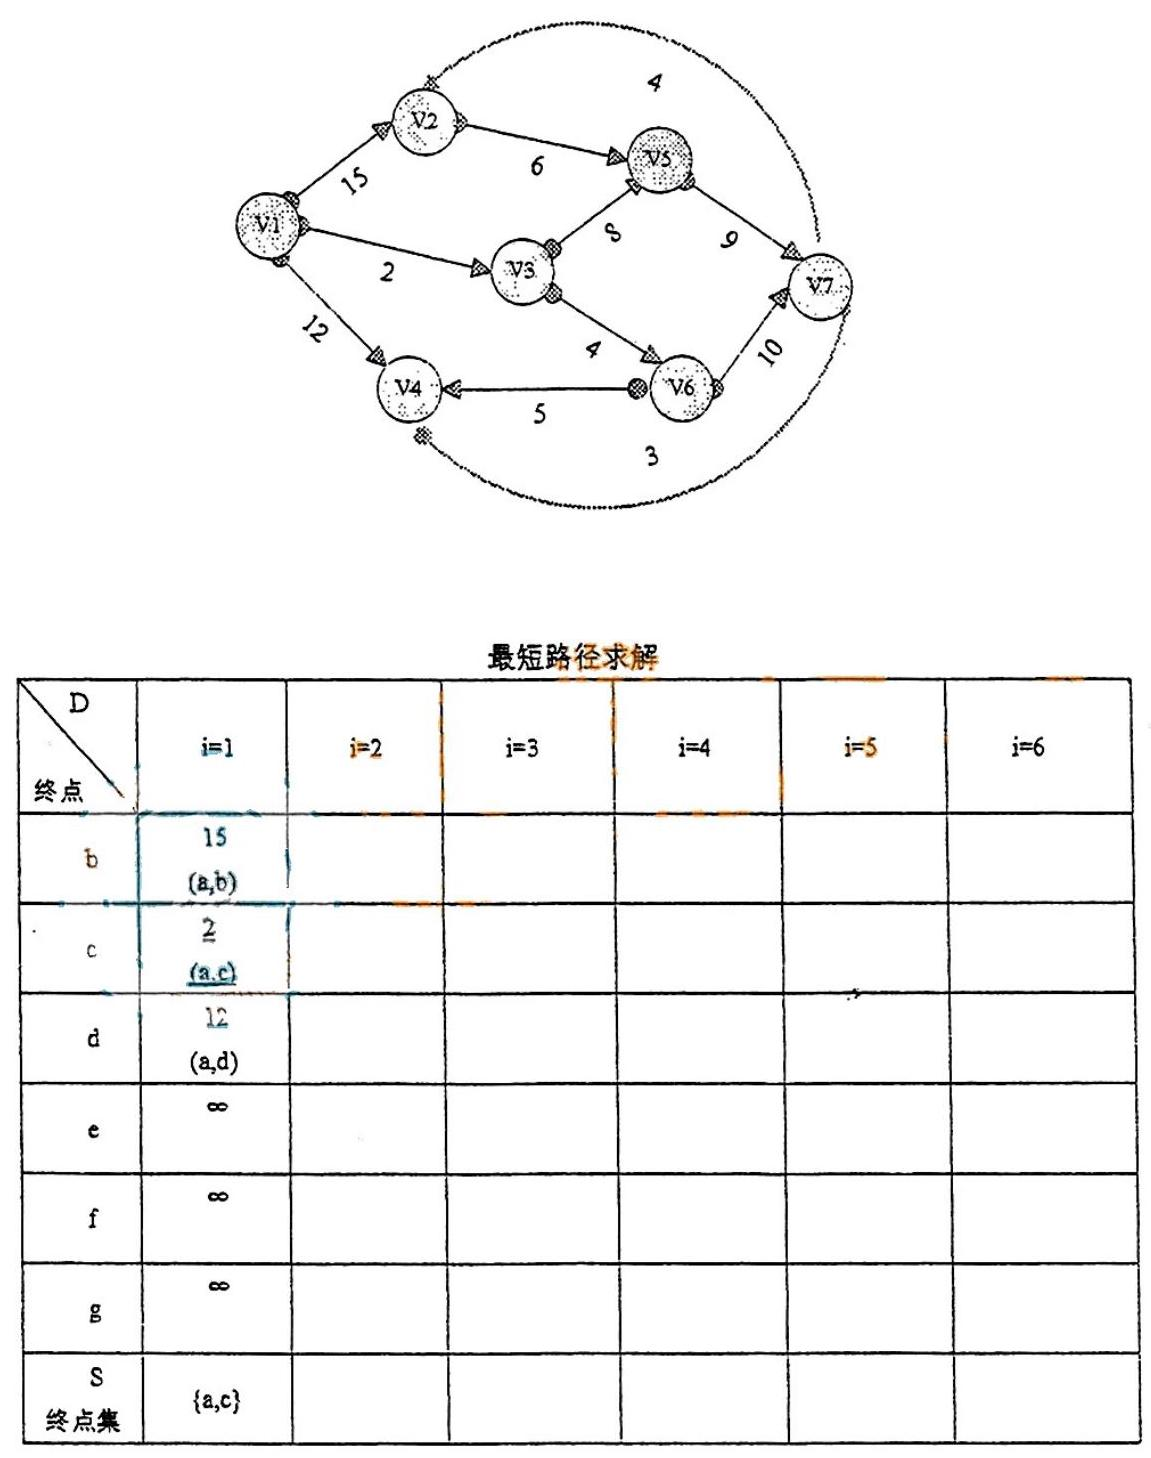
\includegraphics[width=0.9\textwidth]{images/2015/ask_8.jpg}
\end{center}
\vspace{15em}

\section*{四、算法设计、分析题(本大题共 2 小题,每小题 10 分,共 20 分)}

1. 设计一算法, 使得在尽可能少的时间内重排数组, 将所有取负值的关键字放在所有取非负值的关键字之前。

1)先给出算法思想；

2)再描述具体算法, 必要时请给予注释说明；

3)请分析算法的时间复杂度。
\vspace{15em}

2. 设计一算法判断某一二叉树是否为二叉排序树

1)二叉树用二叉链表的形式表示,定义如下:

typedef struct node\{

DataType data;

struct node *lchild,*rchild;

\}BinTNode;

2° 先给出算法思想,再描述算法,必要时请给予注释说明。

\newpage

\chapter{2016}
\section*{一、 选择题(本大题共 20 小题,每小题 2 分,共 40 分)}

1. 下列程序的时间复杂度为 (   )。

\begin{lstlisting}[language=C, basicstyle=\ttfamily]
i=0;s=0;n=100;
while (s<n)
{
    i++;
    s=s+i;
}
\end{lstlisting}

A) \(O\left( \sqrt{n}\right)\) B) \(O\left( \sqrt{2n}\right)\)

C) \(O\left( n\right)\) D) \(O\left( {n}^{2}\right)\)

2. 若线性表的操作主要是查找, 很少涉及到插入、删除操作时, 宜采用以下存储结构较为合适(   )。

A)双链表 B)单链表

C)顺序表 D)循环链表

3. 线性表采用链表存储时地址(   )。

A)必须是连续的 B)连续不连续都可以

C)一定是不连续的 D) 部分地址必须是连续的

4. 若允许表达式内多种括号混合嵌套, 则设计检查表达式中括号是否正确配对的算法,通常选用的辅助结构是(   )。

A) 栈 B)线性表

C) 队列 D) 二叉排序树

5. 若进栈序列为1,2,3,4,5,6,且进栈和出栈可以穿插进行,则不可能出现的出栈序列是(   )。

A)2,4,3,1,5,6 B)3,2,4,1,6,5

C)4,3,2,1,5,6 D)2,3,5,1,6,4

6. 栈和队列的共同点是(   )。

A) 都是先进先出 B) 都是先进后出

C)只允许在端点处插入和删除元素 D) 没有共同点

7. 在长度为 \(\mathrm{n}\) 的顺序表中删除第 \(\mathrm{i}\left( {1 \leq  \mathrm{i} \leq  \mathrm{n}}\right)\) 个元素时,需要移动元素的次数为 (   )。

A) n-i+1 B) i

C) i+1 D) n-i

8. 用链表作为线性表的存储结构的优点是(   )。

A) 便于随机存取 B)花费的存储空间比顺序表少

C)便于插入与删除 D)数据元素的物理顺序与逻辑顺序相同

9. 设循环队列中数组的下标范围是 0 到 n-1 ,其头指针 front 指向队首元素 rear 指向队尾元素,则队列的长度为(   )。

A) rear-front B) rear-front+1

C) (rear-front+1) \% (n-1) D) (rear-front+n+1) \%n): (   ) 0 ) (   ).

10. 二维数组 \(\mathrm{A}\left\lbrack  {12}\right\rbrack  \left\lbrack  {18}\right\rbrack\) 采用列优先的存储方法,若每个元素各占 3 个存储单元, 且 \(\mathrm{A}\left\lbrack  0\right\rbrack  \left\lbrack  0\right\rbrack\) 地址为 150 ,则元素 \(\mathrm{A}\left\lbrack  9\right\rbrack  \left\lbrack  7\right\rbrack\) 的地址为 (   )。

A) 429 B) 432

C) 435 D) 438

11. 含有 10 个结点的二叉树中, 度为 0 的结点数个数为 4 , 则度为 2 的结点个数为(   )。

A) 3 B) 4

C) 5 D) 6

12. 关于树和森林,下列说法错误的是(   )。

A)树的结点数可以为 0

B) 树的度是树内各结点的度的最大值

C) 树的子树可以有顺序, 也可以无顺序

D)二叉树不是树

13. 在一个图中,所有顶点的度数之和等于所有边数的(   )倍。

A) \(1/2\) B) 1

C) 2 D) 4

14. 如果求一个连通图中以某个顶点为根的高度最小的生成树, 应采用 (   )。

A) 深度优先搜索算法 B) 广度优先搜索算法

C)求最小生成树的普里姆算法(Prim 算法) D) 拓扑排序算法

15. 下面哪一方法可以判断出一个有向图是否有环(即回路)(   )。

A) 求节点的度 B)拓扑排序

C) 求最短路径 D) 求关键路径

16. 已知无向图的邻接表如下图所示,根据算法,则从顶点 \({\mathrm{V}}_{0}\) 出发按深度优先遍历的顶点序列是(   )。 A) \({\mathrm{V}}_{1}{\mathrm{\;V}}_{3}{\mathrm{\;V}}_{2}{\mathrm{\;V}}_{0}\) B) V0 V2 V3 V1 C) \({\mathrm{V}}_{0}{\mathrm{\;V}}_{3}{\mathrm{\;V}}_{2}{\mathrm{\;V}}_{1}\) D) \({\mathrm{V}}_{0}{\mathrm{\;V}}_{1}{\mathrm{\;V}}_{2}{\mathrm{\;V}}_{3}\) 注: 所有答案必须写在答题纸上, 试卷上作答无效 !

\begin{center}
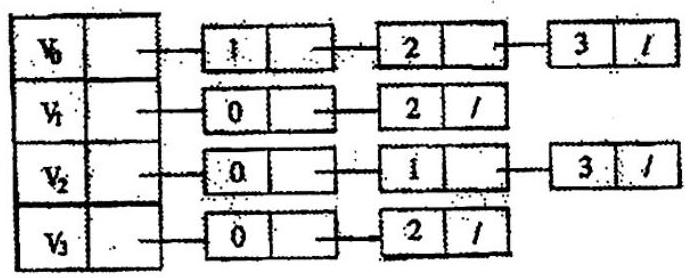
\includegraphics[width=0.5\textwidth]{images/2016/choice_16.jpg}
\end{center}
\hspace*{3em} 

17. 能进行二分查找的线性表,必须以 (   )。

A) 顺序方式存储, 且元素按关键字分块有序

B) 链式方式存储, 且元素按关键字有序

C) 顺序方式存储, 且元素按关键字有序

D) 链式方式存储, 且元素按关键字分块有序

18. 快速排序在下列哪种情况下最易发挥其长处。(   )

A) 被排序的数据中含有多个相同排序码

B) 被排序的数据已基本有序

C) 被排序的数据完全无序

D) 被排序的数据中的最大值和最小值相差悬殊

19. 非空的单循环链表的头指针为 head, 尾指针为 rear, 则下列条件成立的是 (   )。

A) rear->next->next==head B) rear->next==head

C) head->next= = rear D) head->next->next= = rear

20. 已知一个有向图如下图所示,则从顶点 \(\mathrm{a}\) 出发进行深度优先偏历,不可能得到的深度优先遍历序列为(   )。

\begin{center}
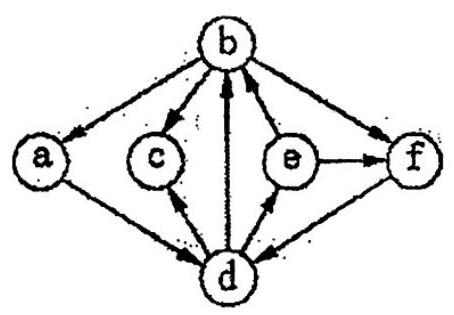
\includegraphics[width=0.3\textwidth]{images/2016/choice_20.jpg}
\end{center}
\hspace*{3em} 

A) a d b e f c

B) a d c e f b

C) a d c b f e

D) a d e f c b

\section*{二、填空题(本大题共 15 小题,每小题 2 分,共 30 分)}

1. 假设长度为 \(\mathrm{n}\) 的顺序表查找每个数据元素的概率相等,即 \({\mathrm{P}}_{\mathrm{i}} = 1/\mathrm{n}\) ,则顺序查找算法的平均查找长度为:\_\_\_\_\_\_\_\_。

2. 设指针变量 \(\mathrm{p}\) 指向单链表中结点 \(\mathrm{A}\) ,则删除结点 \(\mathrm{A}\) 的语句序列为: \(\mathrm{q} = \mathrm{p} -  > \mathrm{{next}}\) ; \(p -  >\) data \(= q -  >\) data; \(p -  >\) next \(=\) \_\_\_\_\_\_\_\_; fee(q)。

3. 设栈 \(\mathrm{S}\) 和队列 \(\mathrm{Q}\) 的初始状态为空,元素 \({\mathrm{S}}_{1},\mathrm{\;S}2,\mathrm{\;S}3,\mathrm{\;S}4,\mathrm{\;S}5,\mathrm{\;S}6\) 将依次入栈 \(\mathrm{S}\) ,一个元素出栈后即进入队列 \(\mathrm{Q}\) 。如果这 6 个元素的出队顺序为 \(\mathrm{S}2,\mathrm{S}3\) , \(\mathrm{S}4,\mathrm{S}6,\mathrm{S}5,\mathrm{S}1\) ,则栈 \(\mathrm{S}\) 的容量至少应该是\_\_\_\_\_\_\_\_,上述过程才不会错。

4. 不论是顺序存储结构的栈还是链式存储结构的栈, 其入栈和出栈操作的时间复杂度均为\_\_\_\_\_\_\_\_(要求填写大 0 表示的时间复杂度)。

5. 假定一棵树的广义表表示为 \(\mathrm{A}\left( {\mathrm{C},\mathrm{D}\left( {\mathrm{E},\mathrm{F},\mathrm{G}}\right) ,\mathrm{H}\left( {\mathrm{I},\mathrm{J}}\right) }\right)\) ,则树的深度为\_\_\_\_\_\_\_\_。

6. 设有 \(\mathrm{n}\) 个结点的完全二叉树,如果按照从自上到下、从左到右从 1 开始顺序编号,则编号为 \(\mathrm{i}\) 的节点的右孩子结点的编号为\_\_\_\_\_\_\_\_。

7. 一棵具有 257 个结点的完全二叉树,它的深度为\_\_\_\_\_\_\_\_。

8. 设某无向图中顶点数和边数分别为 \(\mathrm{n}\) 和 \(\mathrm{e}\) ,所有顶点的度数之和为 \(\mathrm{d}\) ,则 e=\_\_\_\_\_\_\_\_。

9. 具有 100 个叶子节点的哈夫曼树中,其节点总数为\_\_\_\_\_\_\_\_个。

10. 含有 12 个节点的平衡二叉树的最大深度是\_\_\_\_\_\_\_\_(设平衡二叉树的根节点的深度是 i )。

11. 设二叉树 \(\mathrm{T}\) 的前序遍历序列和中序遍历序列分别是: \(\mathrm{b},\mathrm{d},\mathrm{c},\mathrm{a},\mathrm{e},\mathrm{f}\) 和 \(\mathrm{c}\) , \(\mathrm{d},\mathrm{e},\mathrm{a},\mathrm{b},\mathrm{f}\) ; 则其后续遍历序列为\_\_\_\_\_\_\_\_。

12. 设查找表中有 100 个元素,如果用二分法查找方法查找数据元素 \(\mathrm{x}\) ,则最多需要比较\_\_\_\_\_\_\_\_ 次就可以断定数据元素 \(\mathrm{x}\) 是否在查找表中。

13. 设有一稀疏图 G,则 G 采用\_\_\_\_\_\_\_\_(若只考虑采用邻接矩阵或邻接表存储)存储较省空间。

14. 折半查找有序表(4,6,12,20,28,38,50,70,88,100),若查找表中元素20, 它将依次与表中元素\_\_\_\_\_\_\_\_ 比较大小。

15. 在插入和选择排序中,若初始数据基本正序,则选用\_\_\_\_\_\_\_\_排序。

\section*{三、问答题(本大题共 7 小题,每小题 8 分,共 56 分)}

1. 将如题图 1(a) 所示的一棵树转换为对应的二叉树, 并画出二叉树; 将图1(b) 所示的一棵二叉树转换成森林。

\begin{figure}[htbp]
    \centering
    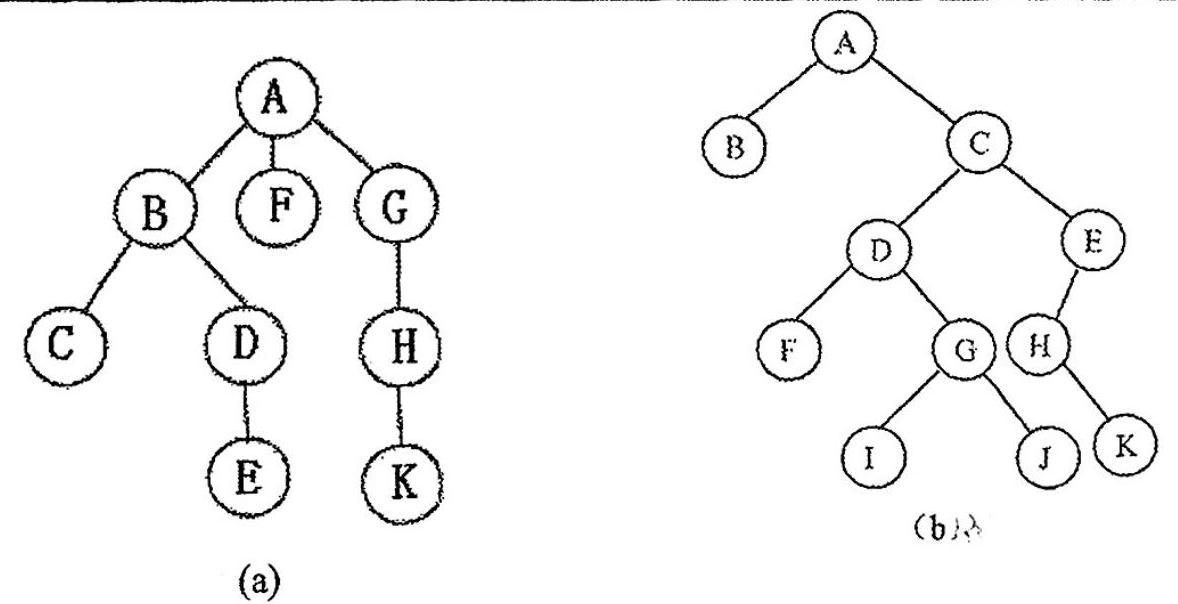
\includegraphics[width=0.3\textwidth]{images/2016/ask_1.jpg}
    \caption*{图1} % 使用带星号的 caption*
\end{figure}
\vspace{15em}

2. 如题图 2 所示有一棵二叉树, 写出该二叉树的先根遍历 (先序遍历) 序列和中根遍历 (中序遍历) 序列。

\begin{figure}[htbp]
    \centering
    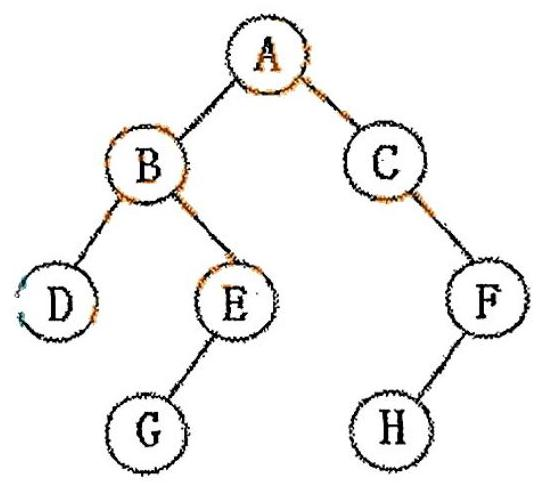
\includegraphics[width=0.3\textwidth]{images/2016/ask_2.jpg}
    \caption*{图2} % 使用带星号的 caption*
\end{figure}
\vspace{15em}

\newpage
3. 如题图 3 矩阵表示一个无向连通网 (其中 \(\infty\) 表示没有边,距离为 \(\infty\) ),试画出它所表示的连通网及该连通网的最小生成树。
\vspace{15em}

4. 如题图 4 是带权的有向图 G,画出其邻接表 (要求:邻接表中) 并根据邻接表写出其深度优先遍历序列。

\begin{figure}[htbp]
    \centering
    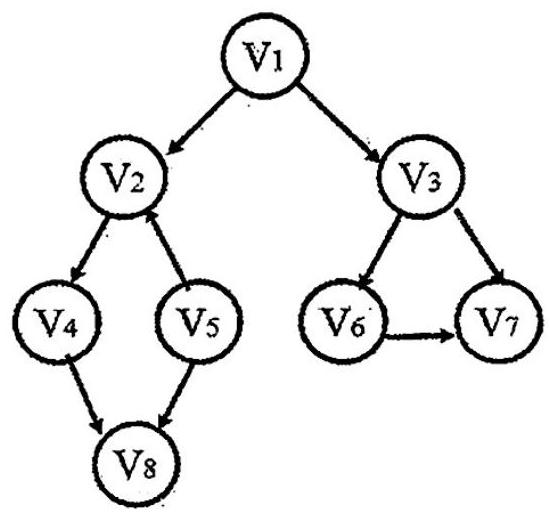
\includegraphics[width=0.3\textwidth]{images/2016/ask_4.jpg}
    \caption*{图4} % 使用带星号的 caption*
\end{figure}
\vspace{15em}

\newpage
5. 试写出一组键值(46,58,15,45,90,18,10,62)应用直接插入排序算法从小到大排序后各趟的结果。
\vspace{15em}

6. 请利用遮杰斯特拉(Dijkstra)算法求出图 5 中从顶点 \({\mathrm{V}}_{0}\) (标号为 0 的顶点) 到其他各项点间的最短路径, 请跟据表中已经完成的寻找第 1 个最短路径的点提示完成下表。

\begin{figure}[htbp]
    \centering
    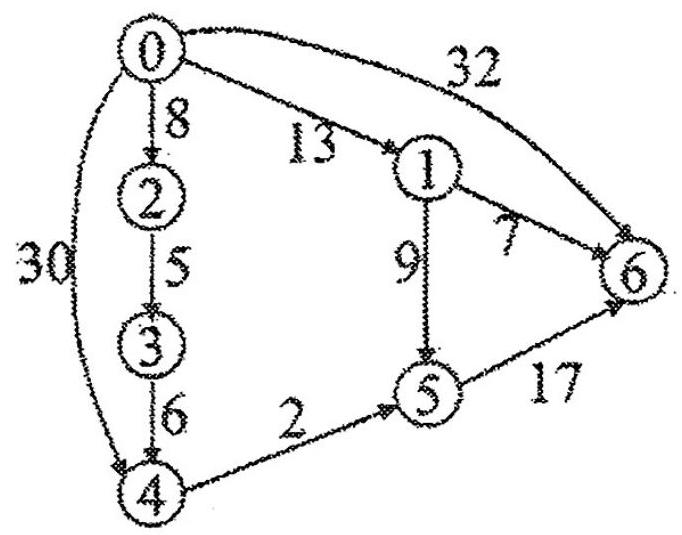
\includegraphics[width=0.3\textwidth]{images/2016/ask_6.jpg}
    \caption*{图5} % 使用带星号的 caption*
\end{figure}

\begin{center}
\begin{tabular}{|c|c|c|c|c|c|c|}
\hline
\multirow{2}{*}{终点} & \multicolumn{6}{|c|}{从 \(\mathrm{{VO}}\) 到各终点的 \(\mathrm{D}\) 值和最短路径的求解过程} \\
\cline{2-7}
 & i=1 & i=2 & i=3 & i=4 & i=5 & i=6 \\
\cline{1-7}
V1 & 13 (V0, V1) & \phantom{X} & \phantom{X} & \phantom{X} & \phantom{X} & \phantom{X} \\
\cline{1-7}
V2 & 8 (V0, V2) & \phantom{X} & \phantom{X} & \phantom{X} & \phantom{X} & \phantom{X} \\
\cline{1-7}
V3 & \(\infty\) & \phantom{X} & \phantom{X} & \phantom{X} & \phantom{X} & \phantom{X} \\
\cline{1-7}
V4 & 30 (V0, V4) & \phantom{X} & \phantom{X} & \phantom{X} & \phantom{X} & \phantom{X} \\
\cline{1-7}
V5 & \(\infty\) & \phantom{X} & \phantom{X} & \phantom{X} & \phantom{X} & \phantom{X} \\
\cline{1-7}
V6 & 32 (V0, V6) & \phantom{X} & \phantom{X} & \phantom{X} & \phantom{X} & \phantom{X} \\
\cline{1-7}
Vj & V2 . & \phantom{X} & \phantom{X} & \phantom{X} & \phantom{X} & \phantom{X} \\
\cline{1-7}
S & \(\{ {V0},{V2}\}\) & \phantom{X} & \phantom{X} & \phantom{X} & \phantom{X} & \phantom{X} \\
\cline{1-7}
\hline
\end{tabular}
\end{center}
\vspace{3em}

\newpage
7. 已知哈希函数为 \(H\left( K\right)  = \left( {3 * K}\right) {\;\operatorname{mod}\;{11}}\) ,采用线性探测再散列解决冲突 \({\mathrm{H}}_{\mathrm{i}} = \left( {\mathrm{H}\left( \mathrm{K}\right)  + \mathrm{{di}}}\right) {\;\operatorname{mod}\;\mathrm{{ll}}}\) ,对下列线性表(6,8,10,17,20,23,53,41,54,57) 求其哈希表。要求将关键字23,53,41,54和 57 依次存入到下面的哈希表中, 并填写相应的探测次数。

答: 哈希表如下:

\begin{center}
\begin{tabular}{|c|c|c|c|c|c|c|c|c|c|c|c|}
\hline
\phantom{X} & 0 & 1 & 2 & 3 & 4 & 5 & 6 & 7 & 8 & 9 & 10 \\
\cline{1-12}
哈希表 & \phantom{X} & \phantom{X} & 8 & \phantom{X} & \phantom{X} & 20 & \phantom{X} & 6 & 10 & 17 & \phantom{X} \\
\cline{1-12}
探测次数 & \phantom{X} & \phantom{X} & 1 & \phantom{X} & \phantom{X} & 1 & \phantom{X} & 1 & 1 & 3 & \phantom{X} \\
\cline{1-12}
\hline
\end{tabular}
\end{center}

\section*{四、算法设计、分析题(本大题共 2 小题,每小题 12 分,共 24 分)}

1. 请设计一个算法,将有 \(n\) 个元素的数组 \(A\) 中的元素 \(A\left\lbrack  0\right\rbrack\) 至 \(A\left\lbrack  {n - 1}\right\rbrack\) 循环右移 \(k\) 位,并要求只用一个元素大小的附加存储,元素移动或交换次数为 \(\mathrm{O}\left( \mathrm{n}\right)\) 。要求先给出算法思想, 再描述算法, 必要时请给予注释和说明。
\vspace{15em}

2. 设计在二叉排序树上查找节点的值等于 key (int 类型) 的节点算法。其中二叉树用二叉链表的形式表示, 定义如下:
\begin{lstlisting}[language=C, basicstyle=\ttfamily]
typedef struct node{
    int key;
    struct node *lchild,*rchild;
}BinNode,*bitree;
\end{lstlisting}


要求先给出算法思想,再描述算法,必要时请给予注释和说明。
\newpage

\chapter{2017}
\section*{一、选择题(本大题共 20 小题,每小题 2 分,共 40 分)}

1. 下面程序段的时间复杂度是 (   )。
\begin{lstlisting}[language=C, basicstyle=\ttfamily]
for(i = 0;i < n;i++)
    for(j = 1;j < m;j++)
        A[i][j] = 0;
\end{lstlisting}

A. O(n) B. \(O\left( {m + n + 1}\right)\) C. \(\mathrm{O}\left( {\mathrm{m} + \mathrm{n}}\right) \;\) D. \(\mathrm{O}\left( {{\mathrm{m}}^{ * }\mathrm{n}}\right)\)

2. 链表不具有的特点是 (   )。

A. 可随机访问任一元素 B. 插入、删除不需要移动元素

C. 不必事先估计存储空间 D. 所需空间与线性表长度成正比

3. 若某栈的输入序列为 \(1,2,3,\ldots ,\mathrm{n}\) ,输出序列的第一个元素为 \(\mathrm{n}\) ,则第 2 个输出元素为(   )。

A. 1 B. n-1 C. n D. 都有可能

4. 判定一个循环队列 \(\mathrm{Q}\) (最多元素为 \(\mathrm{m}\) 个) 为满队列的条件是 (   )。

A. Q. front \(=\) Q. rear B. Q. front \(! =\) Q. rear

C. Q. front \(= \left( {\text{ Q. rear } + 1}\right) \% \mathrm{\;m}\) D. Q.front \(! = \left( {\text{ Q.rear } + 1}\right) \% \mathrm{\;m}\)

5. 设有两个串 \(\mathrm{T}\) 和 \(\mathrm{P}\) ,求 \(\mathrm{P}\) 在 \(\mathrm{T}\) 中首次出现的位置的串运算称作 (   )。

A. 联结 B. 求子串

C. 字符定位 D. 子串定位

6. 将一个 \(\mathrm{A}\left\lbrack  {10}\right\rbrack  \left\lbrack  {10}\right\rbrack\) (下标从 0 开始计算)的矩阵按行优先顺序存放,每个元素占 4 个存储单元,并且 A[0][5]的存储地址是 1020,则 A[7][2]的地址是(   )。

A. 1000 B. 1020 C. 1108 D. 1288

7. 一棵含有 18 个结点的二叉树的高度至少为(   )。

A. 3 B. 4 C. 5 D. 6

8. 已知某非空二叉树采用顺序存储结构, 树中结点的数据信息按完全二叉树的层次序列依次存放在一个一维数组中, 即

\begin{center}
\begin{tabular}{|c|c|c|c|c|c|c|c|c|c|c|c|c|c|c|c|}
\hline
\phantom{X} & A & B & C & \phantom{X} & D & E & F & \phantom{X} & \phantom{X} & G & \phantom{X} & \phantom{X} & H & \phantom{X} & \phantom{X} \\
\cline{1-16}
\hline
\end{tabular}
\end{center}

则该二叉树的后序遍历序列为(   )。

A. G, D, B, E, F, H, C, A B. G, B, D, E, H, C, F, A

C. G, D, B, H, E, F, C, A D. B, G, D, E, H, C, F, A

9. 看不清，没有上传
% 9. 在下列树中,(   )是完全二叉树。 注: 所有答案必须写在答题纸上, 试卷上作答无效 ! 重庆邮电大学 2017 年攻读硕士学位研究生入学考试试题

% \begin{center}
% 
\includegraphics[width=1.0\textwidth]{images/bo_d35oef3ef24c73b45250_1_146_194_1357_251_0.jpg}
% \end{center}
% \hspace*{3em} 

% A

% E

% 0

% D

10. 有 n 个球队参加的某联赛按单循环方式进行比赛,那么共需要进行(   ) 场比赛。

A. \(\mathrm{n}\left( {\mathrm{n} - 1}\right) /2\) B. n C. n(n-1) D. \(\mathrm{n} + 1\)

11. 下列排序算法中,时间复杂度不受数据初始状态影响,恒为 \(\mathrm{O}\left( {{\mathrm{n}}^{ * }{\log }_{2}{}^{\mathrm{n}}}\right)\) 的是 (   )。

A. 快速排序 B. 冒泡排序 C. 直接选择排序 D. 堆排序

12. 若长度为 \(\mathrm{n}\) 的线性表采用顺序存储结构,在其第 \(\mathrm{i}\) 个位置插入一个元素的时间复杂度为(   )(1<=i<=n+1)。

A. \(\mathrm{O}\left( 0\right)\) B. O(1) C. O(n) D. O(n2)

13. 任何一个无向连通图的最小生成树 (   )。

A. 只有一棵 B. 有一棵或多棵 C.一定有多棵 D. 可能不存在

14. 具有 n 个结点的满二叉树,其叶子结点有(   )个。

A. \(\mathrm{n}/2\) B. \(\left( {n - 1}\right) /2\) C. \(\left( {\mathrm{n} + 1}\right) /2\) D. n/2-1

15. 下列排序方法中不稳定的是(   )。

A. 归并排序 B. 快速排序 C. 气泡排序 D. 直接插入排序

16. 如下图,哪一项是该图的拓扑排序 (   )

\begin{center}
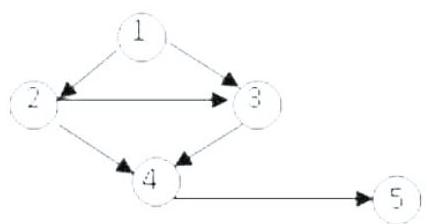
\includegraphics[width=0.3\textwidth]{images/2017/choice_16.jpg}
\end{center}
\hspace*{3em} 

A.1,3,2,4,5 B.1,2,3,4,5

C.1,2,4,3,5 D.1,2,3,5,4

17. 在所有排序方法中,关键字比较的次数与记录的初始排列次序无关的是 (   )。

A. 希尔排序 B. 起泡排序 C. 插入排序 D. 选择排序

18. 若用一个大小为 6 的数组来实现循环队列, 且当前 rear 和 front 的值分别为 0 和 3 。当从队列删除两个元素, 再加入一个元素后, rear 和 front 的值分别为(   )。

A. 1 和 5 B. 2 和 4 C. 4 和 2 D. 5 和 1

19. 已知一个图如下所示,从顶点 \(\mathrm{a}\) 出发进行深度优先遍历可能得到的序列为 (   )。

\begin{center}
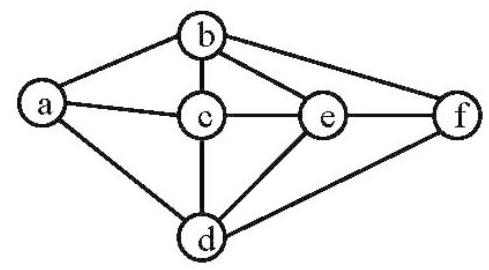
\includegraphics[width=0.4\textwidth]{images/2017/choice_19.jpg}
\end{center}
\hspace*{3em} 

A. acefbd B. acbdfe C. acbdef D. acdbfe

20. 若无向图 \(\mathrm{G}\) 有 7 个顶点,至少需要(   )条边,才能保证该图一定是连通图 (边可依附任两顶点, 但无重复边和自环)。

A. 6 B. 16 C. 31 D. 42

\section*{二、填空题(本大题共 10 小题,每小题 3 分,共 30 分)}

1. 有向图 G 用邻接矩阵 A[1..n,1..n]存储,其第 i 行的所有非 0 元素的个数等于 顶点 \(\mathrm{i}\) 的\_\_\_\_\_。

2. 设栈 \(\mathrm{S}\) 和队列 \(\mathrm{Q}\) 的初始状态皆为空,元素 \(\mathrm{a}1,\mathrm{\;a}2,\mathrm{\;a}3,\mathrm{\;a}4,\mathrm{\;a}5\) 和 \(\mathrm{a}6\) 依次通过一个栈,一个元素出栈后即进入队列 \(\mathrm{Q}\) ,若6个元素出队列的顺序是 \(\mathrm{a}3\) , a5 \(,\mathrm{a}4,\mathrm{a}6,\mathrm{a}2,\mathrm{a}1\) 则栈 \(\mathrm{S}\) 至少应该容纳\_\_\_\_\_个元素。

3. 在一棵二叉树中,度为 0 的结点的个数为 \(\mathrm{n}0\) ,度为 1 的结点的个数为 \(\mathrm{n}1\) , 则该二叉树共有\_\_\_\_\_个结点。

4. 某二叉树的先序遍历序列是 ABDGCEFH, 中序遍历序列是 DGBAECHF, 那么该二叉树的后序遍历序列是\_\_\_\_\_。

5. 表长为 \(\mathrm{n}\) 的线性表,当在任何位置上删除一个元素的概率相等时,删除一个元素需移动元素的平均个数为\_\_\_\_\_。

6. 6 阶 B-树 (B-Tree) 中, 每个结点至多包含 5 个关键码, 除根和叶结点外, 每个结点至少包含\_\_\_\_\_个关键码。

7. 已知完全二叉树的第 10 层(根结点为第 1 层)总共只有 5 个结点, 则其叶子结点数是\_\_\_\_\_。

8. 用顺序存储的方法将完全二叉树中的所有结点逐层存放在数组 \(\mathrm{R}\left\lbrack  {0,..,\mathrm{n} - 1}\right\rbrack\) (下标从 0 开始计) 中,结点 \(\mathrm{R}\left\lbrack  \mathrm{i}\right\rbrack\) 若有双亲节点,则双亲结点的下标是\_\_\_\_\_。

9. 某表达式二叉树按先序遍历的结果为 a, b, c, d,-,*,+, e, f,-,令 a = 6, b = 3, c = 4, d = 2, \(\mathrm{e} = 5,\mathrm{f} = 1\) ,则该表达式的值等于\_\_\_\_\_。

10. G 为无向图,如果从 \(\mathrm{G}\) 的某个顶点出发进行一次遍历,即可访问图的每个顶点,则该图一定是\_\_\_\_\_图。

\section*{三、问答题(本大题共 7 小题,每小题 8 分,共 56 分)}

1. 现有森林如下图, 请画出对应的二叉树。

\begin{center}
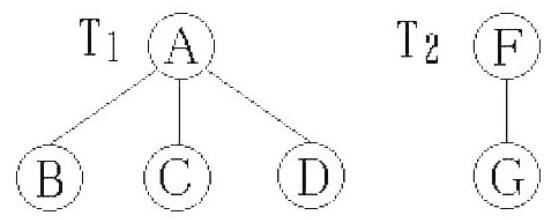
\includegraphics[width=0.4\textwidth]{images/2017/ask_1.jpg}
\end{center}
\hspace*{3em} 
\vspace{10em}

2. 已知某字符串 \(\mathrm{S}\) 中共有 8 种字符,各种字符分别出现 1 次、2 次、7 次、5 次、 4 次、 3 次、 4 次和 9 次,对该字符串用 \(\{ 0,1\}\) 进行前缀编码。

(1)请画出对应的 Huffman 树,并给出各字符的前缀编码； 

(2)请问该字符串 \(\mathrm{S}\) 的编码有多少位？
\vspace{10em}

\newpage
3. 设一个无向网 \(\mathrm{G}\) 的邻接矩阵 \(\mathrm{A}\) 如下:

\[
A = \left\lbrack  \begin{matrix} \infty & \infty & 4 & 2 & \infty & \infty & \infty & \infty \\  \infty & \infty & \infty & \infty & 1 & 7 & \infty & \infty \\  4 & \infty & \infty & \infty & \infty & \infty & 6 & \infty \\  2 & \infty & \infty & \infty & 3 & 0 & 5 & \infty \\  \infty & 1 & \infty & 3 & \infty & \infty & \infty & 8 \\  \infty & 7 & \infty & \infty & \infty & \infty & \infty & 9 \\  \infty & \infty & 6 & 5 & \infty & \infty & \infty & \infty \\  \infty & \infty & \infty & \infty & \infty & 8 & \infty & \infty  \end{matrix}\right\rbrack
\]

(1)请根据给定的邻接矩阵 \(\mathrm{A}\) 画出网 \(\mathrm{G}\) 的图( \(\mathrm{G}\) 中顶点用 \(\mathrm{{vi}}\) 表示)；

(2)如果对某个顶点的邻接点的访问顺序按序号从小到大排列,请写出从顶点 \(\mathrm{v}1\) 出发,按“深度优先”和“广度优先”搜索方法遍历网 \(\mathrm{G}\) 所得到的顶点序列; 

(3)从顶点 v1 出发,按照最小生成树的 Prim 算法,画出网 \(\mathrm{G}\) 的一棵最小生成树。
\vspace{11em}

4. 对一组关键字:49, 38, 65, 97, 76, 13, 27 采用快速排序方法进行排序, 用第一关键字作支点/参考值(pivot),请写出快速排序的第一趟的交换过程。
\vspace{10em}

\newpage
5. 设 Hash 函数为 \(\mathrm{H}\left( \mathrm{K}\right)  = \mathrm{K}{\;\operatorname{mod}\;7}\) ,哈希表的地址空间为0,1,2,3,4,5,6, 开始时哈希表为空,用二次探测再散列法解决冲突,请画出依次插入键值 9 、 14、16、6、23、12、18 后的哈希表。
\vspace{15em}

6. 已知关键字序列为40,35,25,36,70,56,依次将各元素插入到一棵初始为空的二叉排序树, 画出对应的二叉排序树。
\vspace{15em}

\newpage
7. 已知初始序列(52,80,63,44,48,91),写出直接插入排序的各趟排序的结果。 
\vspace{26em}

\section*{四、算法设计、分析题(本大题共 2 小题, 每小题 12 分, 共 24 分)}

1. 试写一算法, 对带头结点的单链表实现就地逆置。

(1)结点结构定义如下:
\begin{lstlisting}[language=C, basicstyle=\ttfamily]
typedef struct node{ //结点类型定义
    int data; //结点的数据域
    struct node *next;
}ListNode,*LinkList;
\end{lstlisting}

(2)先给出算法思想,再描述具体算法,必要时请给予注释说明；
\vspace{20em}

2. 给定某一二叉树的根结点, 请写一个算法判断该树是否为平衡二叉树。

(1)二叉树用二叉链表表示, 定义如下:
\begin{lstlisting}[language=C, basicstyle=\ttfamily]
typedef struct tnode{
    int key;
    struct tnode *lchild,*rchild;
}BinNode,*bitree;
\end{lstlisting}

(2)先给出算法思想,再描述算法,必要时给予注释说明

\newpage

\chapter{2018}
\section*{一、选择题(本大题共 15 小题,每小题 2 分,共 30 分)}

1. 下面程序段的时间复杂度是(   )。
\begin{lstlisting}[language=C, basicstyle=\ttfamily]
i = 1;
while(i <= n)
    i = i*3;
\end{lstlisting}

A.O(n) B. \(O\left( {{nlog}\left( n\right) }\right)\) C. \(\mathrm{O}\left( {\log \left( \mathrm{n}\right) }\right)\) D. \(O\left( {\log }_{3}^{n}\right)\)

2. 在 \(\mathrm{n}\) 个元素的顺序表中插入或删除一个元素,需要平均移动表中(   )个元素。

A. (n) B. \(\left( {\mathrm{n}/2}\right)\) C. \(\left( {\mathrm{n}}^{2}\right)\) D. (1)

3. 设循环队列中数组的下标范围是 \(0,\ldots ,\mathrm{m} - 1\) ,其头指针 front 指向队首元素, rear 指向队尾元素,则队列的长度为(   )。

A. (rear-front +1)\% (m +1) B. (rear-front \(+ \mathrm{m} + 1\) ) \(\% \mathrm{\;m}\)
C. rear-front D. rear-front +1

4. 设计一个十进制转换为八进制的算法,采用(   )数据结构最佳。

A. 栈 B. 队列

C. 顺序结构线性表 D. 链式结构线性表

5. 若某个栈的输入序列为 \(1,2,3,\ldots ,\mathrm{n}\) ,输出序列的第一个元素为 \(\mathrm{n}\) ,则第 \(\mathrm{i}\) 个输出元素为(   )。

A. i B. n-i C. n-i+1 D. 哪个元素无所谓

6. 六个元素按6,5,4,3,2,1的顺序进栈,下列哪个出栈序列是错误的 (   )。

A. 5 4 3 6 1 2 B. 4 5 3 1 2 6

C. 3 4 6 5 2 1 D. 2 3 4 1 5 6

7. 某二叉树的先序序列和后序序列正好相反,则该二叉树一定是(   )二叉树。

A. 空或只有一个结点 B. 高度等于其结点数

C. 任一结点无左孩子 D. 任一结点无右孩子

8. 高度为 \(\mathrm{k}\) 的完全二叉树至少有(   )个结点 ( 空树高度为 0 )。

A. \({2}^{\mathrm{k} - 1}\) B. \({2}^{\mathrm{k}}\)

C. \({2}^{\mathrm{k}} - 1\) D. \(\mathrm{k}\)

9. 设高度为 \(\mathrm{h}\) 的二叉树上只有度为 0 和度为 2 的结点,则此二叉树中至多有 (   )个结点。

A. \({2}^{\mathrm{h}} - 1\) B. \({2}^{h - 1}\) C. \({2}^{\mathrm{h}} + 1\) D. \({2}^{h + 1} - 1\)

10. 数组 A 中,每个元素的长度为 3 个字节,行下标 i 从 1 到 8 ,列下标 j 从 1 到 10 ,从首地址 SA 开始连续存放在存储器内,该数组按行优先存放时,元素 \(\mathrm{A}\left\lbrack  8\right\rbrack  \left\lbrack  5\right\rbrack\) 的起始地址为(   )。

A. SA+141 B. SA+222

C. SA+144 D. SA+225

11. 任何一个无向连通图的最小生成树(   )。

A. 有一棵或多棵 B. 一定只有一棵

C．一定有多棵 D. 可能不存在

12. 对于一个具有 \(\mathrm{n}\) 个顶点和 \(\mathrm{e}\) 条边的无向图,若采用邻接表表示,则表头向量的大小为 \(\mathrm{n}\) ；所有邻接表中的结点总数是(   )。

A. \(\mathrm{e}/2\) B.e C. 2e D.n+e

13. 设结点 \(\mathrm{x}\) 和结点 \(\mathrm{y}\) 是二叉树 \(\mathrm{T}\) 中的任意两个结点,若在先序序列中 \(\mathrm{x}\) 在 \(\mathrm{y}\) 之前,而在后序序列中 \(\mathrm{x}\) 在 \(\mathrm{y}\) 之后,则 \(\mathrm{x}\) 和 \(\mathrm{y}\) 的关系是 (   )

A. \(\mathrm{x}\) 是 \(\mathrm{y}\) 的左兄弟 B. \(\mathrm{x}\) 是 \(\mathrm{y}\) 的右兄弟
C. \(\mathrm{x}\) 是 \(\mathrm{y}\) 的祖先 D. \(\mathrm{x}\) 是 \(\mathrm{y}\) 的后代

14. 关于下面的图形,哪个说法正确(   )。

\begin{center}
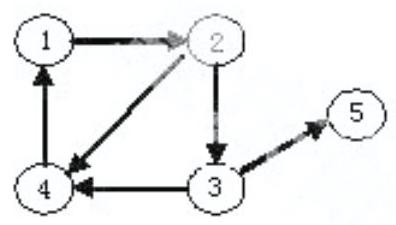
\includegraphics[width=0.3\textwidth]{images/2018/choice_14.jpg}
\end{center}
\hspace*{3em} 

A. 路径 \(< 1,2 > , < 2,4 > , < 4,1 >\) 是一条回路；

B. 顶点 2 的入度为 2 ；

C. 顶点 4 的出度为 2 ；

D. 以上皆非。

15. 下列序列中,(   )是执行第一趟快速排序后得到的序列(排序的关键字类型是字符串)。

A. \(\left\lbrack  {\mathrm{{da}},\mathrm{{ax}},\mathrm{{eb}},\mathrm{{de}},\mathrm{{bb}}}\right\rbrack\) ff \(\left\lbrack  {\mathrm{{ha}},\mathrm{{gc}}}\right\rbrack\) B. \(\left\lbrack  {{cd},{eb},{ax},{da}}\right\rbrack\) ff \(\left\lbrack  {{ha},{gc},{bb}}\right\rbrack\)

C. \(\left\lbrack  {\mathrm{{gc}},\mathrm{{ax}},\mathrm{{eb}},\mathrm{{cd}},\mathrm{{bb}}}\right\rbrack\) ff \(\left\lbrack  {\mathrm{{da}},\mathrm{{ha}}}\right\rbrack\) D. \(\left\lbrack  {{ax},{bb},{cd},{da}}\right\rbrack\) ff \(\left\lbrack  {{eb},{gc},{ha}}\right\rbrack\)

\section*{二、填空题(本大题共 10 小题,每小题 3 分,共 30 分)}

1. 采用顺序查找方法查找长度为 \(\mathrm{n}\) 的线性表时,在等概率情况下查找成功的平均查找长度为\_\_\_\_\_。

2. 已知数据表 A 中每个元素距其最终位置不远,则采用\_\_\_\_\_排序算法最节省时间。

3. 图 G 是一个非连通图,共有 28 条边,则该图至少有\_\_\_\_\_个顶点。

4. 设一循环队列 \(Q\) 中, rear 指针指向队尾元素的下一个位置, front 指针指向队首元素,则判断队列中元素为空的条件是\_\_\_\_\_。

5. 在大根堆中,关键字最小的元素可能存放在堆的任一\_\_\_\_\_结点上。

6. 某后缀表达式为 abcd-*+ef/-,令 a=2, b=3, c=4, d=5, e=6, f=2,则该表达

式的值等于\_\_\_\_\_。

7. 有 \(\mathrm{n}\) 个顶点的连通图用邻接矩阵表示时,该矩阵至少有\_\_\_\_\_个非零元素。

8. 高度(空树高度为 0)为 5 的 AVL 树,其结点数最少是\_\_\_\_\_。

9. 广义表((a),((b), c),(((d))))的长度是\_\_\_\_\_,深度是\_\_\_\_\_。

10. 在有 n 个结点的二叉链表中,空链域的个数为\_\_\_\_\_。

\section*{三、问答题(本大题共 6 小题,每小题 10 分,共 60 分)}

1. 已知二叉树的先序序列和中序序列分别为 ABDGCEFH 和 DGBAECHF:

(1) 画出该二叉树；

(2)写出此二叉树的后序序列；

(3)画出与此二叉树对应的森林。
\vspace{15em}

2. 图 G 各顶点的连接关系及相应权值如下图所示:

(1)画出图的邻接矩阵存储图示；

(2)从顶点 1 开始对图进行广度优先遍历,写出遍历结果；

(3)使用 Kruskal 算法求该图的最小生成树,给出形成过程。

\begin{center}
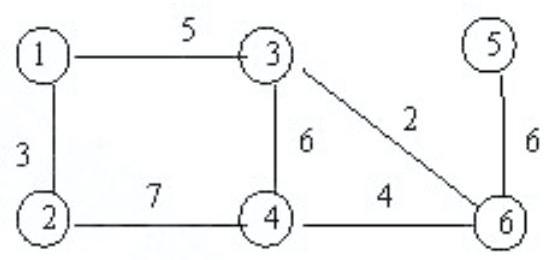
\includegraphics[width=0.4\textwidth]{images/2018/ask_2.jpg}
\end{center}
\hspace*{3em} 
\vspace{15em}

\newpage
3. 设散列表的长度为 8 ,散列函数 \(\mathrm{H}\left( \mathrm{k}\right)  = \mathrm{k}{\;\operatorname{mod}\;7}\) ,初始记录关键字序列为 (25,31,8,27,13,68),要求:

(1)分别给出用线性探测法和链地址法作为解决冲突方法的过程；

(2)计算(1)中两种解决冲突方法的平均查找长度。
\vspace{15em}

4. 已知一个图的顶点集 \(\mathrm{V}\) 和边集 \(\mathrm{E}\) 分别为:

\(\mathrm{V} = \{ 1,2,3,4,5,6,7\}\) ;

\(E = \{  < 2,1 > , < 3,2 > , < 3,6 > , < 4,3 > , < 4,5 > , < 4,6 > , < 5,1 > , < 5,7 > , < 6,1 > , < 6,2 > , < 6,5 > \} ;\)

若存储它采用邻接表, 并且每个顶点邻接表中的边结点都是按照终点序号从小到大的次序链接的,

(1)画出该图的邻接表存储图示；

(2)按拓朴排序算法进行排序,试给出得到的拓扑排序的序列。
\vspace{15em}

\newpage
5. 假设一个线性链表的类名为 linkedList, 链表结点的类名为 ListNode, 它包含两个数据成员 data 和 link。data 存储该结点的数据, link 是链接指针。下面给定一段递归打印一个链表中所有结点中数据的算法:

void PrintList (ListNode *L) \{

\hspace*{1em} if (L != NULL) \{

\hspace*{3em} printf("\%d ", L->data);

\hspace*{3em} PrintList (L->link);

\hspace*{1em} \}

\}

试问此程序在什么情况下不实用? 给出具体修改后的可实用的程序？
\vspace{15em}

6. 对于如下图所示的 AOE 网络,计算各活动弧的 \(e\left( {a}_{i}\right)\) (活动 \({a}_{i}\) 的最早开始时间)和 \(1\left( {a}_{j}\right)\) (活动 \({a}_{j}\) 的最迟开始时间)函数值、各事件(顶点)的 \({ve}\left( {v}_{i}\right)\) (事件 \({v}_{i}\) 的最早发生时间)和 \({vl}\left( {v}_{j}\right)\) (事件 \({v}_{j}\) 的最迟发生时间)函数值; 列出各条关键路径。

\begin{center}
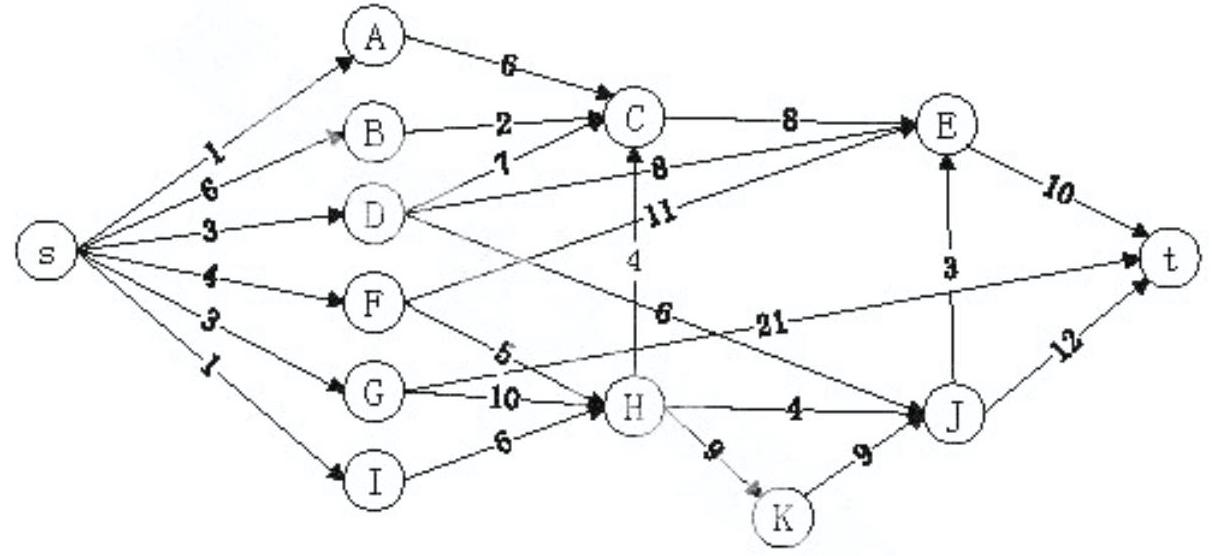
\includegraphics[width=1.0\textwidth]{images/2018/ask_6.jpg}
\end{center}
\hspace*{3em} 
\vspace{15em}

\section*{四、问答题(本大题共 2 小题,每小题 15 分,共 30 分)}

1. 现有关键字序列 \(\{ {45},{24},{37},{53},{12},{93},{47},{60}\}\) ,按以下要求完成:

(1)根据给定的关键字序列构造一棵二叉查找(排序)树,以二叉链表形式存储, 进行中序遍历可以得到从小到大排列的有序序列, 请写出构造过程 (不要求算法)。

(2)在(1)的基础上,请编写一个函数(int LeafCount(Binary\_tree BT),

求此二叉树的叶子结点个数。

有关的数据结构已描述如下:
\begin{lstlisting}[language=C, basicstyle=\ttfamily]
typedef struct { //二叉树结点
    int data;
    Binary_node *left;
    Binary_node *right;
} Binary_node, *Binary_tree;

int LeafCount(Binary_tree bt); //计算树bt的叶结点的个数
\end{lstlisting}
\vspace{45em}

2. 下面给出一个排序算法,其中 \(\mathrm{n}\) 是数据类型为 Type 的数组 \(\mathrm{A}\left\lbrack  \right\rbrack\) 中元素总数。

\begin{lstlisting}[language=C, basicstyle=\ttfamily]
void unknown(Type a[], int n)
{
    int d = 1;
    int j;
    while (d < n / 3)
        d = 3 * d + 1;
    while (d > 0)
    {
        for (int i = d; i < n; i++)
        {
            Type temp = a[i];
            j = i;
            while (j >= d && a[j - d] > temp)
            {
                a[j] = a[j - d];
                j = j - d;
            }
            a[j] = temp;
        }
        d /= 3;
    }
}
\end{lstlisting}



(1)阅读此算法,说明它的功能；

(2)对于下面给出的整数数组,追踪第一趟 while \(\left( {\mathrm{d} > 0}\right)\) 内的每次 for 循环结束时数组中数据的变化。(为清楚起见,本次循环未涉及的不移动的数据可以不写出, 每行仅写出一个 for 循环的变化);

\begin{center}
\begin{tabular}{|c|c|c|c|c|c|c|c|c|c|c|c|}
\hline
\multirow{2}{*}{步} & a[0] & a[1] & a[2] & a[3] & a[4] & a[5] & a[6] & a[7] & a[8] & a[9] & \multirow{2}{*}{移动 次数} \\
\cline{2-11}
 & 77 & 44 & 99 & 66 & 33 & 55 & 88 & 22 & 44 & 11 &  \\
\cline{1-12}
1 & \phantom{X} & \phantom{X} & \phantom{X} & \phantom{X} & \phantom{X} & \phantom{X} & \phantom{X} & \phantom{X} & \phantom{X} & \phantom{X} & \phantom{X} \\
\cline{1-12}
2 & \phantom{X} & \phantom{X} & \phantom{X} & \phantom{X} & \phantom{X} & \phantom{X} & \phantom{X} & \phantom{X} & \phantom{X} & \phantom{X} & \phantom{X} \\
\cline{1-12}
... & \phantom{X} & \phantom{X} & \phantom{X} & \phantom{X} & \phantom{X} & \phantom{X} & \phantom{X} & \phantom{X} & \phantom{X} & \phantom{X} & \phantom{X} \\
\cline{1-12}
\hline
\end{tabular}
\end{center}

( 3 )以上各次循环的数据移动次数分别是多少。


\newpage

\chapter{2019}
\section*{一、选择题(本大题共 10 小题,每小题 2 分,共 20 分)}

1. 对于双向循环链表, 每个结点有两个指针域 next 和 prior, 分别指向前驱和后继。在 \(\mathrm{p}\) 指针所指向的结点之后插入 \(\mathrm{s}\) 指针所指结点的操作应为(   )。

A. p->next = s; s->prior = p; p->next->prior = s; s->next = p->next;

B. p->next = s; p->next->prior = s; s->prior = p; s->next;

C. s->prior = p; s->next = p->next; p->next = s; p->next->prior = s;

D. s->prior = p; s->next = p->next; p->next->prior = s; p->next = s;

2. 由 abc,3 个结点可以构造出多少种不同的二叉树? (   )

A. 2 B. 3 C. 4 D. 5

3. 设有数组 \(\mathrm{A}\left\lbrack  {\mathrm{i},\mathrm{j}}\right\rbrack\) ,数组的每个元素长度为 3 字节, \(\mathrm{i}\) 的值为1到 \(8,\mathrm{j}\) 的值为 1 到 10 , 数组从内存首地址 BA 开始顺序存放, 当用以列为主存放时, 元素 A[5, 8]的存储首地址为(   )。

A. BA+141 B. BA+180 C. BA+222 D. BA+225

4. 一个栈的输入序列为 123 ,则下列序列中不可能是栈的输出序列的是(   )。

A.231 B. 3 2 1

C. 3 1 2 D. 1 2 3

5. 下述编码中哪一个不是前缀码(   )。

A.(00,01,10,11) B.(0,1,00,11)

C.(0,10,110,111) D.(1,01,000,001)

6. 当一棵有 n 个结点的二叉树按层次从上到下,同层次从左到右将数据存放在一维数组 A[l..n]中时,数组中第 i 个结点的左孩子为(   )。

A. \(\mathrm{A}\left\lbrack  {2\mathrm{i}}\right\rbrack  \left( {2\mathrm{i} =  < \mathrm{n}}\right)\) B. \(\mathrm{A}\left\lbrack  {2\mathrm{i} + 1}\right\rbrack  \left( {2\mathrm{i} + 1 =  < \mathrm{n}}\right)\) C. \(A\left\lbrack  {i/2}\right\rbrack\) D. 无法确定

7. 假设一个有 \(\mathrm{n}\) 个顶点和 \(\mathrm{e}\) 条弧的有向图用邻接表表示,则删除与某个顶点 vi 相关的所有弧的时间复杂度是(   )。

A. O(n) B. \(\mathrm{O}\left( \mathrm{e}\right)\) C. \(\mathrm{O}\left( {\mathrm{n} + \mathrm{e}}\right)\) D. \(\mathrm{O}\left( {{\mathrm{n}}^{ * }\mathrm{e}}\right)\)

8. 串的长度是指(   )。

A. 串中所含不同字母的个数 B. 串中所含字符的个数

C. 串中所含不同字符的个数 D. 串中所含非空格字符的个数

9. 循环队列存储在数组 \(\mathrm{A}\left\lbrack  {0..\mathrm{m}}\right\rbrack\) 中,则入队时的操作为(   )。

A. rear=rear+1 B. rear=(rear+1) mod (m-1)

C. rear=(rear+1) mod m D. rear=(rear+1)mod(m+1)

10. 关键路径是事件结点网络中(   )。

A. 从源点到汇点的最长路径 B. 从源点到汇点的最短路径

C. 最长回路 D. 最短回路

\section*{二、填空题(本大题共 15 小题,每空 2 分,共 40 分)}

1. 中缀算式 (3+4X) -2Y/3 对应的后缀算式为\_\_\_\_\_。

2. 在完全二叉树中,编号为 \(\mathrm{i}\) 和 \(\mathrm{j}\) 的两个结点处于同一层的条件是\_\_\_\_\_。

3. 构造 n 个结点的强连通图,至少有\_\_\_\_\_条弧。

4. 设有一个空栈,栈顶指针为 \({1000}\mathrm{H}\) (十六进制),现有输入序列为 \(\mathrm{a},\mathrm{b},\mathrm{c},\mathrm{d}\) ,
e. 经过 PUSH, PUSH, POP, PUSH, POP, PUSH, PUSH 之后,输出序列是\_\_\_\_\_, 而栈顶指针值是\_\_\_\_\_ \(\mathrm{H}\) 。设栈为顺序栈,每个元素占 4 个字节。

5. 若串 S1=‘ABCDEFG’, S2=‘9898’, S3=‘\#\#\#’, S4=‘012345’, 执行 concat(replace(S1, substr(S1, length(S2), length(S3)), S3), substr(S4, index(S2,‘8’), lengt h(S2))),其结果为\_\_\_\_\_。

6. 若一组记录的排序码为(46,79,56,38,40,84),则利用堆排序的方法建立的初始堆为\_\_\_\_\_。

7. 在有序表 (12,24,36,48,60,72,84) 中二分查找关键字 72 时所需进行的关键字比较次数为\_\_\_\_\_。

8. 有向图的边集为 \(\{  < \mathrm{a},\mathrm{c} > , < \mathrm{a},\mathrm{e} > , < \mathrm{e},\mathrm{b} > , < \mathrm{e},\mathrm{d} > , < \mathrm{b},\mathrm{d} > , < \mathrm{d},\mathrm{c} > , < \mathrm{c},\mathrm{f} > \}\) ,该图的一个拓扑排序为:\_\_\_\_\_。

注:所有答案必须写在答题纸上, 试卷上作答无效 !

9. 当输入序列局部有序或元素个数较小时, 在快速排序、选择排序、插入排序、 归并排序、堆排序中,最佳的排序方法是\_\_\_\_\_。

10. 假设两个队列共享一个循环向量空间 (参见右图), 其类型 Queue2 定义如下:

\begin{center}
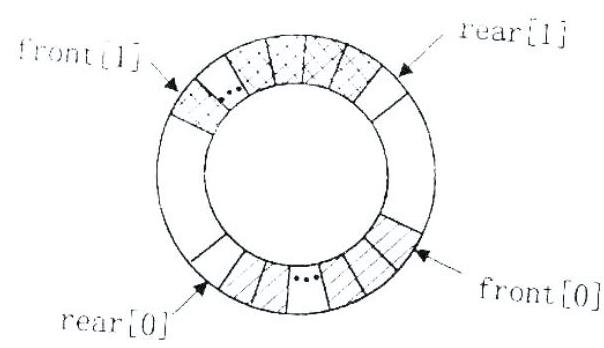
\includegraphics[width=0.5\textwidth]{images/2019/blank_10.jpg}
\end{center}
\hspace*{3em} 

\begin{lstlisting}[language=C, basicstyle=\ttfamily]
    typedef struct {
        DateType data[MaxSize];
        int front[2],rear[2];
    } Queue2;
\end{lstlisting}

对于i=0或l,front[i]的和rear[i]的分别为第i个队列的头指针和尾指针。请对以下算法填空，实现第i个队列的入队操作。

\begin{lstlisting}[language=C, basicstyle=\ttfamily]
int EnQueue(Queue2 *Q,int i,DateType x)
{    //若第i个队列不满，则元素x入队列，并返回1：否则返回0
    if(i<0 || i>1)
        return 0;
    if(Q->rear[i]==Q->front[          ]) return 0;
    Q->data[          ]=x;
    Q->rear[i]=[          ];
    return1;
}
\end{lstlisting}


11. 高度为 8 的平衡二叉树的结点数至少有\_\_\_\_\_个。

12. 文件由\_\_\_\_\_组成；记录由\_\_\_\_\_组成。

13. 对于一个具有 \(\mathrm{n}\) 个结点的单链表,在已知的结点*p 后插入一个新结点的时间复杂度为\_\_\_\_\_,在给定值为 \(\mathrm{x}\) 的结点后插入一个新结点的时间复杂度为\_\_\_\_\_。

14. 在 n 个记录的有序顺序表中进行折半查找,最大比较次数是\_\_\_\_\_。 

15. 求从某源点到其余各顶点的 Dijkstra 算法在图的顶点数为 10 ,用邻接矩阵表示图时计算时间约为 10ms,则在图的顶点数为 40,计算时间约为\_\_\_\_\_ms。

\section*{三、问答题(本大题共 6 小题,每小题 10 分,共 60 分)}

1. 一个线性表为 B=(12,23,45,57,20,03,78,31,15,36),设散列表为 \(\mathrm{{HT}}\left\lbrack  {0.12}\right\rbrack\) ,散列函数为 \(\mathrm{H}\left( \mathrm{{key}}\right)  = \mathrm{{key}}\% {13}\) 并用线性探查法解决冲突,请画出散列表, 并计算等概率情况下查找成功的平均查找长度。
\vspace{10em}

2. 已知二叉树的存储结构为二叉链表,阅读下面算法。

\begin{lstlisting}[language=C, basicstyle=\ttfamily]
typedef struct node {
    DateType data;
    struct node *next;
} ListNode;
typedef ListNode *LinkList;
LinkList Leafhead = NULL;
void Inorder (BinTree T)
{
    LinkList s;
    if(T)
    {
        Inorder(T->lchild);
        if ((!T->lchild)&&(!T->rchild))
            {
                s=(ListNode*)malloc(sizeof(ListNode));
                s->data = T->data;
                s->next = Leafhead;
                Leafhead=s;
            }
        Inorder(T->rchild);
    }
}
\end{lstlisting}

对于如下所示的二叉树
\begin{center}
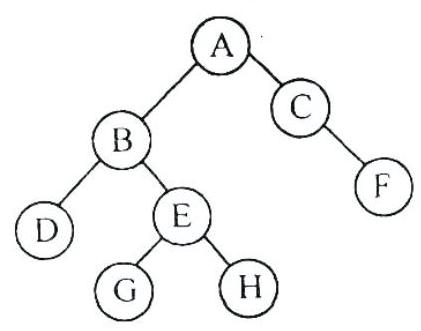
\includegraphics[width=0.4\textwidth]{images/2019/ask_2.jpg}
\end{center}
\hspace*{3em} 

(1)画出执行上述算法后所建立的结构

(2)说明该算法的功能
\vspace{10em}

\newpage
3. 假设以 I 和 O 分别表示入栈和出栈操作。栈的初态和终态均为空,入栈和出栈的操作序列可表示为仅由 \(\mathrm{I}\) 和 \(\mathrm{O}\) 组成的序列,称可以操作的序列为合法序列, 否则称为非法序列。

(1)下面所示的序列中哪些是合法的?

A. IOIIOIOO B. IOOIOIIO C. IIIOIOIO D. IIIOOIOO

(2)通过对(1)的分析,写出一个算法,判定所给的操作序列是否合法。(假定被判定的操作序列已存入一维数组 char A[ ]中, 若操作序列合法, 返回 true, 否则返回 false)。
\vspace{10em}

4. 已知一个连通图如下图所示, 试给出图的邻接矩阵和邻接表存储示意图,若从顶点 \(\mathrm{v}1\) 出发对该图进行遍历, 分别给出一个按深度优先遍历和广度优先遍历的顶点序列.

\begin{center}
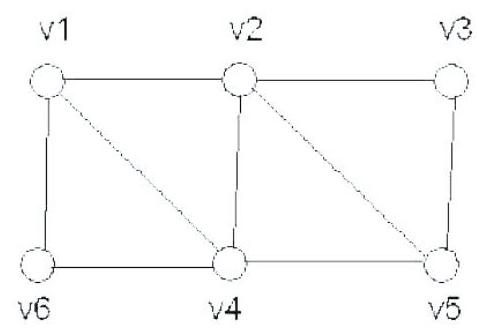
\includegraphics[width=0.4\textwidth]{images/2019/ask_4.jpg}
\end{center}
\hspace*{3em} 

(1)图的邻接矩阵

(2)邻接表存储示意图

(3)从 v1 开始的深度优先遍历的顶点序列

(4)分析在深度遍历过程中,分别使用邻接矩阵和邻接表存储的算法复杂度

( 5 )讨论在图遍历问题中,这两种存储方式的优劣 
\vspace{10em}

\newpage
5. 一棵二叉树的先序序列为 ABCDGEF, 中序序列为 CBDGAFE。 

(1)请画出该二叉树

(2)将二叉树转换为相应的森林
\vspace{10em}

6. 请阅读下列算法,回答问题
\begin{lstlisting}[language=C, basicstyle=\ttfamily]
sort(r,n)
{
    for (i=2;i<=n;i++)
    { 
        x=r[i]; r[0]=x; j=i-1;
        while(x<r[j])
            {
                r[j+1]=r[j];
                j=j-1;
            }
        r[j+1]=x;
    }
}
\end{lstlisting}

(1)这是什么类型的排序算法, 该排序算法稳定吗?

(2)设置 \(\mathrm{r}\left( 0\right)\) 的作用是什么？

(3)若将 while 语句中判断条件改为 \(x <  = r\left( j\right)\) ,该算法将会有什么变化？

(4)若将 while 语句中判断条件改为 \(x <  = r\left( j\right)\) ,该算法是否还能正确工作?
\vspace{10em}

\section*{四、程序设计题 (本大题共 2 小题, 每小题 15 分, 共 30 分)}

1. 设有大小不等的 \(\mathrm{n}\) 个数据组,其数据总量为 \(\mathrm{m}\) ,顺序存放在空间 \(\boxtimes  \mathrm{D}\) 内,每个数据占一个存储单元,数据组的首地址由数组 \(\mathrm{S}\) 给出,(如下图所示),试编写将新数据 \(\mathrm{x}\) 插入到第 \(\mathrm{i}\) 个数据组的末尾且属于第 \(\mathrm{i}\) 个数据组的算法,插入后,空间区 \(\mathrm{D}\) 和数组 \(\mathrm{S}\) 的相互关系仍保持正确。

\begin{center}
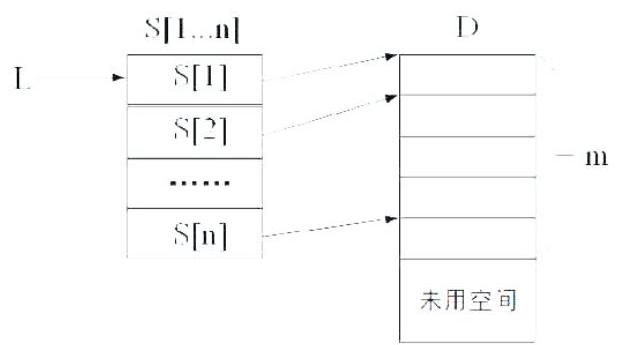
\includegraphics[width=0.5\textwidth]{images/2019/program_1.jpg}
\end{center}
\hspace*{3em} 
\vspace{15em}

2. 快速排序算法中, 如何选取一个界值 (又称为轴元素), 影响着快速排序的效率, 而且界值也并不一定是被排序序列中的一个元素。例如, 我们可以用被排序序列中所有元素的平均值作为界值。用 \(\mathrm{C}\) 语言编写算法实现以平均值为界值的快速排序方法(注:待排序数据存储在数组 \(\mathrm{R}\left\lbrack  \right\rbrack\) 中,数组最小下标为 \(\mathrm{S}\) ,数组最大下标为 T)。
\newpage

\chapter{2020}
\section*{一、选择题(本大题共 15 小题,每小题 2 分,共 30 分)}

1. 设三个函数 \(\mathrm{f},\mathrm{g},\mathrm{h}\) 分别为 \(\mathrm{f}\left( \mathrm{n}\right)  = {1000}{\mathrm{n}}^{3} + {\mathrm{n}}^{2} + {1000},\mathrm{\;g}\left( \mathrm{n}\right)  =\)  \({1000}{n}^{3} + {5000}{n}^{2},h\left( n\right)  = {n}^{3/2} + {5000}{nl}{gn}\) ,下列哪个关系不成立 (\_\_\_\_\_)。

A. \(\mathrm{f}\left( \mathrm{n}\right)  = \mathrm{O}\left( {\mathrm{g}\left( \mathrm{n}\right) }\right)\) B. \(\mathrm{g}\left( \mathrm{n}\right)  = \mathrm{O}\left( {\mathrm{f}\left( \mathrm{n}\right) }\right)\)

C. \(\mathrm{h}\left( \mathrm{n}\right)  = \mathrm{O}\left( {\mathrm{n}}^{3/2}\right)\) D. \(\mathrm{h}\left( \mathrm{n}\right)  = \mathrm{O}\left( {\mathrm{{nl}}\mathrm{{gn}}}\right)\)

2. 已知 \(\mathrm{P}\) 结点是某双向链表的一个结点,在 \(\mathrm{P}\) 结点后插入一个新结点 \(\mathrm{S}\) 的语句序列是(\_\_\_\_\_)。

A. S->prior=P->prior;
P->prior=S;
S->next=P;
P->prior->next=S;

B.
S->prior=P;
S->next=P->next;
P->next->prior=S;
P->next=S;

C.
S->prior=P->prior;
P->prior->next=S;
P->prior=S;
S->next-=P;

D.
S->prior=P;
S->next=P->next;
P->next=S;
P->next->prior=S;

3. 栈在(\_\_\_\_\_)中应用。

A. 递归调用 B. 子程序调用

C. 表达式求值 D. A, B, C

4. 若用一个大小为 6 的数组来实现循环队列, 且当前 rear 和 front 的值分别为 0 和 3 , 当从队列中删除一个元素, 再加入两个元素后, rear 和 front 的值分别为(\_\_\_\_\_)。

A. 1 和 5 B. 2 和 4 C. 4 和 2 D. 5 和 1

5. 设完全二叉树的第 \(\mathrm{i} = 6\) 层有 24 个叶结点,则此树最多有 (\_\_\_\_\_)个结点。( \(i \geq  1\) )

A. 55 B. 79 C. 81 D. 127

6. 下列序列(\_\_\_\_\_)不是堆？

A.12,35,39,57,86,48,42,73,66,100

B.12,70,33,65,24,56,48,92,86,33

C.06,12,20,30,52,23,42,38,103,97,66,56

D.05,23,20,35,28,38,29,61,56,76,40,100

7. 将下图中二叉树按中序线索化,结点 \(\mathrm{f}\) 的右指针和结点 \(\mathrm{g}\) 的左指针分别指向结点 (\_\_\_\_\_)。

\begin{center}
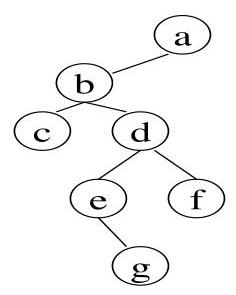
\includegraphics[width=0.2\textwidth]{images/2020/choice_7.jpg}
\end{center}
\hspace*{3em} 

A. d, e B. b, d

C. \(\mathrm{d},\mathrm{b}\) D. \(\mathrm{a},\mathrm{e}\)

8. 在 Huffman 编码中, 若编码长度只允许小于等于 5 , 则除了已对两个字符编码为 0 和 10 外,还可以最多对(\_\_\_\_\_) 个字符编码。

A. 5 B. 6 C. 7 D. 8

9. 设 \(\mathrm{G}\) 是一个非连通无向图,有 28 条边,则该图的顶点数至少有(\_\_\_\_\_)个。

A. 7 B. 8 C. 9 D. 10

10. 对于一个有向图,若一个顶点的度为 \(\mathrm{k}1\) ,出度为 \(\mathrm{k}2\) ,则对应逆邻接表中该顶点的入边表中的边结点数为(\_\_\_\_\_)。

A. k1 B. k2 C. k1-k2 D. \(\mathrm{k}1 + \mathrm{k}2\)

11. 在下图中所示的 AOE (Activity On Edge) 网中, 关键路径长度为(\_\_\_\_\_)。

A. 23 B. 22 C. 16 D. 13

\begin{center}
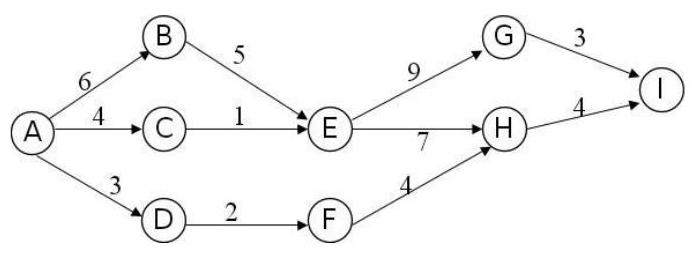
\includegraphics[width=0.5\textwidth]{images/2020/choice_11.jpg}
\end{center}
\hspace*{3em} 

12. 如果一个有向图具有拓扑有序序列, 并且顶点按拓扑有序序列编号,那么其邻接矩阵必定为(\_\_\_\_\_)。

A. 对称矩阵 B. 三对角矩阵

C.上三角矩阵 D. 下三角矩阵

13. 已知一个长度为 18 的有序顺序表中, 若采用折半查找法查找第 12 个元素,则比较次数是(\_\_\_\_\_)。

A. 3 B. 4 C. 5 D. 6

14. 如果将学校所有同学按照生日(不考虑年份,只考虑月、日) 来排序,那么下列排序算法中排序速度最快的算法是 (\_\_\_\_\_)。

A. 归并排序 B. 希尔排序

C. 快速排序 D. 基数排序

15. 下列(\_\_\_\_\_)不是 AVL 树(平衡二叉树)。

A
\begin{center}
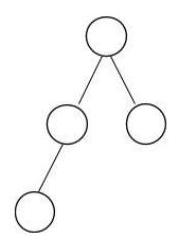
\includegraphics[width=0.2\textwidth]{images/2020/choice_15_A.jpg}
\end{center}
B
\begin{center}
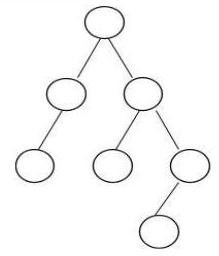
\includegraphics[width=0.2\textwidth]{images/2020/choice_15_B.jpg}
\end{center}
C
\begin{center}
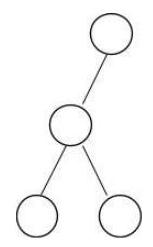
\includegraphics[width=0.2\textwidth]{images/2020/choice_15_C.jpg}
\end{center}
D
\begin{center}
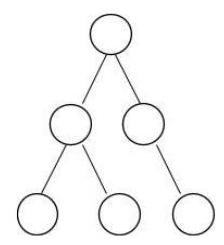
\includegraphics[width=0.2\textwidth]{images/2020/choice_15_D.jpg}
\end{center}

\section*{二、填空题 (本大题共 15 小题, 每小题 2 分, 共 30 分)}

1. 考虑函数 \(f\left( n\right)  = n\log n\) 和 \(g\left( n\right)  = {n}^{a}\) ,其中 \(a\) 是实数。在下列空白处填写合适的数学符号(比如 \(> , \geq  , < , \leq\) 等),使得下列函数关系成立。 \(\mathrm{f} = \mathrm{O}\left( \mathrm{g}\right)\) :当 \(\mathrm{a}\) \_\_\_\_\_1； \(\mathrm{g} = \mathrm{O}\left( \mathrm{f}\right)\) :当 \(\mathrm{a}\) \_\_\_\_\_1。

2. 表达式 a*b-c-d\$e\$f-g-h*i 中,运算符的优先级由高到低依次为 \(- , * ,\$\) ,且均右结合,则相应的后缀式是\_\_\_\_\_。

3.7 个元素 \(\mathrm{a}\) 、 \(\mathrm{b}\) 、 \(\mathrm{c}\) 、 \(\mathrm{d}\) 、 \(\mathrm{e}\) 、 \(\mathrm{f}\) 和 \(\mathrm{g}\) 顺序入栈。在栈上做了 5 次弹出操作,每个出栈的元素被插入到一个队列中。从队列中删除 3 个元素并将其推回到栈中。现在, 从栈中弹出一个元素, 弹出的这个元素是\_\_\_\_\_。

4. 设一个稀疏矩阵有 1000 行 850 列, 其中有 1000 个非 0 数据元素。设每个整数值占 \(2\mathrm{\;B}\) ,数据元素值占 \(4\mathrm{\;B}\) ,则用三元组表存储该矩阵时所需字节数是\_\_\_\_\_。

5. 一棵二叉排序树 (BST, binary search/sort tree) 的后序遍历序列是15,10,23,25,20,35,42,39,30。请给出这棵树的前序遍历序列:\_\_\_\_\_。

6. 如果 T1 是由有序树 \(\mathrm{T}\) 转换成的二叉树,那么 \(\mathrm{T}\) 中结点的后根遍历顺序对应 T1 中结点的\_\_\_\_\_ 遍历。

7. 设一棵树中只有度为 0 和度为 3 的结点,则该树的第 \(\mathrm{i}\) 层 \(\left( {i \geq  1}\right)\) 的结点个数最多为\_\_\_\_\_。

8. 在一个图中, 所有顶点的度数之和等于图的边数的\_\_\_\_\_倍。

9. 一个有向图的邻接表存储如下图所示, 现按深度优先搜索方式从顶点 \(\mathrm{F}\) 出发执行一次遍历,则得到的顶点系列是\_\_\_\_\_。

\begin{center}
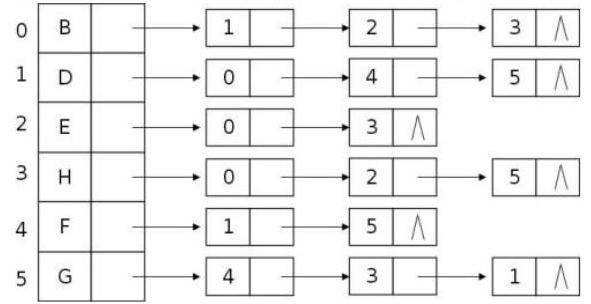
\includegraphics[width=0.5\textwidth]{images/2020/blank_9.jpg}
\end{center}
\hspace*{3em} 

10. 设一个 \(\mathrm{n}\) 个顶点的带权连通图有 \({\mathrm{n}}^{1/2}\log \mathrm{n}\) 条边,则应该选用\_\_\_\_\_(从 Prim, Kruskal 中选择一个填空)算法求这个图的最小生成树, 从而使计算时间较少。

11. 对于长度为 9 的有序顺序表, 若采用折半查找, 在相等查找概率情况下查找成功的平均查找长度为\_\_\_\_\_,查找不成功的平均查找长度为\_\_\_\_\_。

12. 将 10 个元素散列到大小可容 100000 个元素的散列表中,\_\_\_\_\_产生冲突。(请在“一定会”、“一定不会”、“仍然可能会”这些术语中选择正确的进行填空)

13. 数组 \(A\) 中,每个元素 \(A\) 的长度为 3 个字节,行下标 \(i\) 从 1 到 8, 列下标 \(j\) 从 1 到 10,从首地址 1000 开始连续存放在存储器内, 该数组按行优先存放时,元素 \(A\left\lbrack  8\right\rbrack  \left\lbrack  5\right\rbrack\) 的起始地址为\_\_\_\_\_。

\vspace{14em}

14. 如果有一个时间复杂度为 \(\mathrm{O}\left( {\mathrm{n}}^{2}\right)\) 的算法(比如冒泡排序、选择排序或插入排序等),在有 200 个元素的数组上运行需要耗时 3.2 毫秒。那么, 在类似的有 40000 个元素的数组上运行, 需要\_\_\_\_\_秒时间。

15. 顺序文件中,要存取第 i 个记录,必须先存取\_\_\_\_\_个记录。

\section*{三、综合应用题 (本大题共 6 小题, 每小题 10 分, 共 60 分)}

\begin{enumerate}
    \item 下面这段 C 代码, 针对输入的简单算术表达式的后缀表达式, 输出其计算结果。例如, 输入 \texttt{5 2 * 3 3 2 + * +}, 该程序输出 25。请给出缺失的 5 行代码。

\begin{lstlisting}[escapechar=@]
#include <stdio.h>
#include <ctype.h>

#define EOF -1
void push(int); /* push the argument on the stack */
int pop(void); /* pop the top of the stack */
void flagError();

int main()
{
    int c, m, n, r;
    while ((c = getchar()) != EOF)
    {
        if (isdigit(c))
        {
            @\underline{\hspace{4cm} (1) \hspace{4cm}}@;
        }
        else if ((c == '+') || (c == '*'))
        {
            m = @\underline{\hspace{3cm} (2) \hspace{3cm}}@;
            n = @\underline{\hspace{3cm} (3) \hspace{3cm}}@;
            r = (c == '+') ? n + m : n * m;
            @\underline{\hspace{4cm} (4) \hspace{4cm}}@;
        }
        else if (c != ' ')
        {
            flagError();
        }
    }
    printf("%c", @\underline{\hspace{4cm} (5) \hspace{4cm}}@);
}
\end{lstlisting}
\end{enumerate}


2. 一个二叉树 BT 有 10 个结点, BT 为指向树根结点的指针, 其值为 6, Lchild, Rchild 分别为结点的左、右孩子指针域, data 为结点的数据域。各结点的存储结构如下表所示:

\begin{center}
\begin{tabular}{|c|c|c|c|c|c|c|c|c|c|c|}
\hline
\phantom{X} & 1 & 2 & 3 & 4 & 5 & 6 & 7 & 8 & 9 & 10 \\
\cline{1-11}
Lchild & 0 & 0 & 2 & 3 & 7 & 5 & 8 & 0 & 10 & 1 \\
\cline{1-11}
Data & J & H & F & D & B & A & C & E & G & I \\
\cline{1-11}
\hline
\end{tabular}
\end{center}

\begin{center}
\begin{tabular}{|c|c|c|c|c|c|c|c|c|c|c|}
\hline
Rchild & 0 & 0 & 0 & 9 & 4 & 0 & 0 & 0 & 0 & 0 \\
\cline{1-11}
\hline
\end{tabular}
\end{center}

请完成下列各题:

( 1 )画出二叉树 BT 的逻辑结构；

(2)写出按前序、中序、后序遍历该二叉树所得到的结点序列；

( 3 )画出二叉树的后序线索树。
\vspace{14em}

\newpage
3. 当输入大小为 \(\mathrm{N}\) 时,您为一个程序收集其相应的运行时间。下表记录了在不同的输入 \(\mathrm{N}\) 情况下,该程序对应的运行时间。

\begin{center}
\begin{tabular}{|c|c|}
\hline
N(输入大小) & Time(运行时间) \\
\cline{1-2}
125 & 0.03 sec \\
\cline{1-2}
1000 & 1.00 sec \\
\cline{1-2}
8000 & 32.00 sec \\
\cline{1-2}
64000 & 1024.00 sec \\
\cline{1-2}
512000 & 32768.00 sec \\
\cline{1-2}
\hline
\end{tabular}
\end{center}

请给出以 \(\mathrm{N}\) 作为输入的函数来估计该程序的运行时间(以秒为单位)。提示: \({\log }_{\mathrm{b}}\mathrm{a} = \mathrm{{lg}}\mathrm{a}/\mathrm{{lg}}\mathrm{b}\)
\vspace{15em}

4. 一个有向图 \(\mathrm{G}\) 的带权邻接矩阵如下所示:

\begin{center}
\begin{tabular}{|c|c|c|c|c|c|}
\hline
\phantom{X} & \({\mathrm{V}}_{1}\) & \({\mathrm{V}}_{2}\) & \({\mathrm{V}}_{3}\) & \({\mathrm{V}}_{4}\) & \({\mathrm{V}}_{5}\) \\
\cline{1-6}
\({\mathrm{V}}_{1}\) & 0 & 16 & 00 & 00 & 21 \\
\cline{1-6}
\({\mathrm{V}}_{2}\) & ① & 0 & 13 & ① & \(\infty\) \\
\cline{1-6}
\({\mathrm{V}}_{3}\) & \(\infty\) & 00 & 0 & 18 & 33 \\
\cline{1-6}
\({\mathrm{V}}_{4}\) & 19 & 00 & 15 & 0 & \(\infty\) \\
\cline{1-6}
\({\mathrm{V}}_{5}\) & 00 & 11 & oo & 00 & 0 \\
\cline{1-6}
\hline
\end{tabular}
\end{center}

请采用单源点最短路径算法 Dijkstra 求解图 \(\mathrm{G}\) 中 \({\mathrm{V}}_{1}\) 点到其他各点的最短路径,要求给出计算过程。
\vspace{14em}

\newpage
5. 设有关键字序列 12,15,23,56,35,48,5,86,9,68,哈希函数为 \(\mathrm{H}\left( \mathrm{{Key}}\right)  = \mathrm{{Key}}{\;\operatorname{mod}\;{11}}\) ,哈希表的地址空间为 \(0 \sim  {10}\) ,开始时哈希表为空, 采用链地址法解决冲突, 请画出依次插入关键字后的哈希表——同一链表中结点对应关键字从小到大有序。
\vspace{14em}

6. 下表 1 中第 0 行是待排序序列的原始输入(365401851 229 963 842 794 176 538); 最后一行为排序后的序列 (176229365401538 794842 851 963 )；其他各行是 5 种排序算法得到的某个中间步骤的内容。表 2 列出了这 5 种排序算法。请按行序直接给出每行序列对应的排序算法的编号。每个数字只使用一次。

\begin{center}
\begin{tabular}{|c|c|c|c|c|}
\hline
\multicolumn{2}{|c|}{行号排序算法序列} & \phantom{X} & \phantom{X} & \phantom{X} \\
\cline{1-5}
第 0 行 & 原始输入365 401 851 229 963 842 794 176 538 & \phantom{X} & \phantom{X} & \phantom{X} \\
\cline{1-5}
第 1 行 & 365 401 851 229 963 842 794 176 538 & \phantom{X} & \phantom{X} & \phantom{X} \\
\cline{1-5}
第 2 行 & 365 401 229 851 963 794 842 176 538 & \phantom{X} & \phantom{X} & \phantom{X} \\
\cline{1-5}
第 3 行 & 365 401 794 176 538 963 842 851 229 & \phantom{X} & \phantom{X} & \phantom{X} \\
\cline{1-5}
第 4 行 & 176 229 365 851 963 842 794 401 538 & \phantom{X} & \phantom{X} & \phantom{X} \\
\cline{1-5}
第 5 行 & 176 229 851 401 963 842 794 365 538 & \phantom{X} & \phantom{X} & \phantom{X} \\
\cline{1-5}
第 6 行 & 排好序的输出176 229 365 401 538 794 842 851 963 & \phantom{X} & \phantom{X} & \phantom{X} \\
\cline{1-5}
\hline
\end{tabular}
\end{center}

\begin{center}
\begin{tabular}{|c|c|c|c|}
\hline
算法编号 & 算法名称 & 算法编号 & 算法名称 \\
\cline{1-4}
1 & 希尔排序(增量为 5,3,1) & 4 & 归并排序 \\
\cline{1-4}
2 & 快速排序 & 5 & 直接插入排 序 \\
\cline{1-4}
3 & 直接选择排序 & 6 & 冒泡排序 \\
\cline{1-4}
\hline
\end{tabular}
\end{center}
\vspace{14em}

\section*{四、算法设计题 (本大题共 2 小题, 每小题 15 分, 共 30 分)}

1. 设以带头结点的双向循环链表表示的线性表为 \(L = \left( {{a}_{1},{a}_{2},{a}_{3},\ldots }\right.\) , \(\left. {a}_{n}\right)\) 。试写一时间复杂度 \(O\left( n\right)\) 的算法,将 \(L\) 改造为 \(L = \left( {{a}_{1},{a}_{3},\ldots ,{a}_{n},\ldots }\right.\) , \(\left. {{\mathrm{a}}_{4},{\mathrm{a}}_{2}}\right)\) 。要求:

(1)描述算法的基本设计思想；

(2)根据设计思想,采用 \(\mathrm{C}\) 语言描述算法,关键之处给出注释。
\vspace{15em}

2. ORDER 公司是一个专门为人们提供排序服务的公司, 该公司的宗旨是:“秩序是最美丽的”。他们的工作是通过一系列移动, 将某些物品按顺序摆好。他们的服务是通过工作量来计算的, 即移动东西的次数。所以, 在工作前必须先考察工作量, 以便向用户提出收费价格。

用户并不知道精确的移动次数, 实质上, 大多数人是凭感觉来认定这一列物品的混乱程度。根据 ORDER 公司的经验, 人们一般是根据 “逆序对” 的数目多少来称呼这一序列的混乱程度。 假设我们将序列中第 \(\mathrm{i}\) 件物品的参数定义为 \({\mathrm{A}}_{\mathrm{i}}\) ,那么排序就是指将 \({A}_{1},{A}_{i},{A}_{n}\) 按从小到大的顺序排序。若 \(i < j\) 且 \({A}_{i} > {A}_{j}\) ,则 \(< i,j >\) 就为一个“逆序对”。

例如: 数组(3,1,4,5,2)的 “逆序对” 有 \(< 3,1 > \text{ 、 } < 3,2 > \text{ 、 } < 4,2 >\) 、 <5,2>,共 4 个。

现在, OEDER 公司请你写一个程序, 在尽量短的时间内, 统计出 “逆序对” 的数目。程序输入 \(\mathrm{n},{\mathrm{A}}_{1},\ldots ,{\mathrm{A}}_{\mathrm{i}},\ldots ,{\mathrm{A}}_{\mathrm{n}},1 \leq  \mathrm{n} \leq  {30000},{\mathrm{A}}_{\mathrm{i}}\) 为小于 200 的正整数。输出序列 \({\mathrm{A}}_{1},\ldots ,{\mathrm{A}}_{\mathrm{i}},\ldots ,{\mathrm{A}}_{\mathrm{n}}\) 的 “逆序对” 数目,即 “逆序数”。并请分析你设计的算法的时间复杂度。

\newpage

\chapter{2021}
\section*{一、 选择题(本大题共 15 小题,每小题 2 分,共 30 分)}

1 设 \(N\) 是描述问题规模的非负整数,下列程序段的时间复杂度是 (   )。

static int fun(int N) \{

if (N == 1) return 0 ;

return 1 + fun(N/2);

\}

A. \(O\left( {\log N}\right)\) B. \(O\left( N\right)\) C. \(\left( {N\log N}\right)\) D. \(O\left( {N}^{2}\right)\)

2 一些随机产生的数采用线性链表存储, 在下面这些排序方法中, (   )的时间复杂度是最小的。

A. 插入排序 B. 快速排序 C. 堆排序 D. 归并排序

3 一个栈的输入序列为 \(a,b,c,d,e\) ,则下列序列中不可能是栈的输出序列的是 (   )。

A. \({b c d a e}\) B. \({e d a c b}\) C. \({b c a d e}\) D. \({a e d c b}\)

4 实现一个队列需要(   )个栈。

A. 1 B. 2 C. 3 D. 4

5 下面(   )是一颗满二叉树的结点个数。

A. 8 B. 13 C. 14 D. 15

6 若 \(\mathrm{X}\) 是二叉中序线索树中一个有左孩子的结点,且 \(\mathrm{X}\) 不为根, 则 \(\mathrm{X}\) 的前驱为(   )。

A. \(\mathrm{X}\) 的双亲 \hspace{2em} B. X 的右子树中最左的结点

C. \(\mathrm{X}\) 的左子树中最右的结点 D. \(\mathrm{X}\) 的左子树中最右的结点

7 下列序列中, 哪一个是堆 (   )

A.75,65,30,15,25,45,20,10

B.75,65,45,10,30,25,20,15

C.75,45,65,30,15,25,20,15

D.75,45,65,10,25,30,20,15

8 一棵 Huffman 树共有 203 个结点, 对其 Huffman 编码, 共能得到(   )个不同的码字。

A. 100 B. 102 C. 200 D. 203

9 下面说法错误的是(   )。

A. 一个有 n 个顶点和 n 条边的无向图一定是有环的。

B. 建立十字链表的时间复杂度和建立邻接表是相同的。

C. 邻接表只能用于有向图的存储,邻接矩阵对于有向图和无向图的存储都适用。

D. 在某些图的应用问题中, 如果需要找到表示同一条边的两个结点, 那么采用邻接多重表比邻接表作为储存结构更为适宜。

10 图的广度优先遍历算法中使用队列作为其辅助数据结构, 那么在算法执行过程中每个顶点进队次数最多为(   )。

A. 1 B. 2 C. 3 D. 4

11 设一个有向图 \(G = \left( {V,E}\right)\) ,其中

\(V = \left\{  {{v}_{1},{v}_{2},{v}_{3},{v}_{4},{v}_{5},{v}_{6}}\right\}\)

\(E = \left\{  { < {v}_{1},{v}_{2} > , < {v}_{2},{v}_{3} > , < {v}_{3},{v}_{6} > , < {v}_{4},{v}_{2} > , < {v}_{4},{v}_{5} > , < {v}_{5},{v}_{6} > }\right\}\)

不属于该图的拓扑排序有序序列是(   )。

A. \({v}_{1}{v}_{2}{v}_{3}{v}_{4}{v}_{5}{v}_{6}\) B. \({v}_{1}{v}_{4}{v}_{2}{v}_{3}{v}_{5}{v}_{6}\)

C. \({v}_{4}{v}_{5}{v}_{1}{v}_{2}{v}_{3}{v}_{6}\) D. \({v}_{4}{v}_{1}{v}_{2}{v}_{3}{v}_{5}{v}_{6}\)

12 判断一个有向图是否存在回路, 除可利用拓扑排序方法外, 还可以用 (   )。

A. 求关键路径的方法 B. 求最短路径的方法

C. 广度优先遍历的方法 D. 深度优先遍历的方法

13 设有一个二叉排序树 (二叉查找树), 其结点上存储有数字 1 到 100 。现在需要查找数字 55 ,下面(   )序列不可能是查找过程中访问过的结点序列。

A. \(\{ {10},{75},{64},{43},{60},{57},{55}\}\) B. \(\{ {90},{12},{68},{34},{62},{45},{55}\}\)

C. \(\{ 9,{85},{47},{68},{43},{57},{55}\}\) D. \(\{ {79},{14},{72},{56},{16},{53},{55}\}\)

14 在顺序表 \(\{ 2\) 、5、7、10、14、15、18、23、35、41、 \({52}\}\) 中, 用二分法查找关键码 12 需做(   )次关键码比较。

A. 2 B. 3 C. 5 D. 4

15 一颗 3 阶 B-树中有 2047 个关键字, 包括叶结点层, 该树的最大深度为 (   )。

A. 11 B. 12 C. 13 D. 14

\section*{二、填空题(本大题共 10 小题,每小题 3 分,共 30 分)}

16 一颗深度为 \(k\) 的平衡二叉树,其每个非终端结点的平衡因子均为 0 ,则该树共有(   )个结点。

17 设 \( Q \) 表示一个包含十六个元素的队列，\( S \) 为一个空栈。  
Head(Q) 返回队列 \( Q \) 的队头元素，但不将其从队列中移除；  
Top(S) 返回栈 \( S \) 的栈顶元素，但不将其从栈中移除。  

考虑如下算法：
\begin{lstlisting}[language=C, basicstyle=\ttfamily]
while Q != NULL
    if S == NULL 或 Top(S) <= Head(Q)
        x := Dequeue(Q);
        Push(S, x);
    else
        x := Pop(S);
        Enqueue(Q, x);
    end
end
\end{lstlisting}

该算法中，while 循环的最大可能执行次数是（   ）。

18 对于模式串“aabaac”,给出其 next 数组:(   )。

19 现有按中序遍历二叉树的结果为 \({abc}\) ,有 (   ) 种不同形态的二叉树可以得到这一遍历结果。

20 设一棵二叉树有 20 个叶子结点, 则在该树中有 2 个孩子的结点个数为(   )。

21 设 \(\mathrm{G}\) 是一个非连通无向图,有 10 条边,则该图的顶点数至少有(   )个。

22 顺序查找 3 个元素的顺序表, 若查找第 1 、第 2 和第 3 个元素的查找概率分布是 \(1/2\) 、 \(1/3\) 和 \(1/6\) ,则查找任一元素的平均查找长度为 (   )。

23 散列函数有一个共同的性质, 即函数值应当以 (   ) 取其值域的每个值。(请在最大概率、最小概率、平均概率、同等概率这些术语中选择正确的进行填空)

24 假设某算法在输入规模为 \(n\) 时的计算时间为 \(\mathrm{T}\left( n\right)  = {n}^{2}\) 。在某台计算机上实现并完成该算法的时间为 \(t\) 秒。现有另一台计算机, 其运行速度为第一台计算机的 64 倍, 那么在这台计算机上用同一算法在 \(t\) 秒内能解输入规模 (   ) 的问题。

25 表达式 \(a \times  b - c - d\$ e\$ f - g - h \times  i\) 中,运算符的优先级由高到低依次为一,×,\$,均右结合,则相应的后缀式是(   )。

\section*{三、综合应用题 (本大题共 7 小题, 共 60 分)}

26 (10分) 假设称正读和反读都相同的字符序列为“回文”,例如,'abba'和'abcba'是回文,'abcde'和'ababab'则不是回文。下面代码判别读入的一个以‘@’为结束符的字符序列是否是“回文”。请给出缺失的 5 行代码。

Status SymmetryString(char* p)

\{



Queue q;

if(!InitQueue(q)) return 0;

Stack s;

InitStack(s);

ElemType e1, e2;

while(\_\_\_\_\_(1)\_\_\_\_\_)\{

\hspace*{4em} Push(s,*p);

\hspace*{4em} EnQueue(q,*p);

\hspace*{7em} ( 2 )\_\_\_\_\_

\}

while(!StackEmpty(s))\{

\hspace*{8em} (3)

\hspace*{4em} (4)

注:所有答案必须写在答题纸上,试卷上作答无效！ 第 5 页/共 9 页

\hspace*{2em} if(\_\_\_\_\_(5)\_\_\_\_\_) return FALSE;

\hspace*{1em} \}

\hspace*{1em} return OK;

\}

27.(5 分)阅读下面代码:

\begin{lstlisting}[language=C, basicstyle=\ttfamily]
int count = 0;
int N = a.length;
sort(a);
for(int i = 0;i < N;i++) {
    for(int j = i + 1;j < N;j++) {
        if(BinarySearch(a, a[i]+a[j])) count++;
    }
}
\end{lstlisting}


假设当 \(\mathrm{N} = {3500}\) ,上述代码运行 1 秒。那么,当 \(\mathrm{N} = {35000}\) 时,

该代码的运行时间最接近下面那个时间？请给出简单的分析过程。

A.10 seconds B. 20 seconds D. 2 minutes

E. 1 hour F. 2 hours
\vspace{10em}

\newpage
28(8 分)将关键字序列 \(\{ {23},{14},9,6,{30},{12},{18}\}\) 散列存储到散列表中, 散列表的存储空间是一个下标从 0 开始的一维数组, 散列函数为 \(\mathrm{H}\left( \mathrm{{Key}}\right)  = \mathrm{{Key}}\mathrm{{MOD}}7\) ,处理冲突采用线性探测法,要求装填(载)因子为 0.7 。

请画出所构造的散列表。
\vspace{10em}

29 (12 分) 已知一棵二叉树的先序序列: ABDGJEHCFIKL, 中序序列: DJGBEHACKILF。

(1)画出此二叉树的形态。

(2)画出此二叉树的后序线索树。

(3)采用孩子兄弟表示法来存储该二叉树,请画出此二叉树的存储结构。

(4)画出与此二叉树对应的森林。
\vspace{10em}

\newpage
30 (8分) 考虑下列36个字符 (symbol) 的序列: FC F C E C A C

BDEDFEABFBAFFCDCBEDFFFCCDEEF 下面表 30-1 给出了为上述字符序列编码的四种变长编码方式, 即 CODE1、CODE2、CODE3、CODE4; 表 30-2 给出了编码特点, 即 \(\mathrm{A}\text{ 、 }\mathrm{\;B}\text{ 、 }\mathrm{C}\text{ 、 }\mathrm{D}\) ,请给出这 4 种编码方式所具有的编码特点。(填写该编码方式具有的编码特点编号即可,不用给出具体分析过程) 

表 30-1:

\begin{center}
\begin{tabular}{|c|c|c|c|c|c|}
\hline
symbol & frequency & CODE1 & CODE2 & CODE3 & CODE4 \\
\cline{1-6}
A & 3 & 011 & 011 & 1110 & 100 \\
\cline{1-6}
B & 4 & 010 & 010 & 1111 & 101 \\
\cline{1-6}
C & 8 & 00 & 00 & 00 & 01 \\
\cline{1-6}
D & 5 & 110 & 101 & 110 & 110 \\
\cline{1-6}
E & 6 & 001 & 100 & 10 & 111 \\
\cline{1-6}
F & 10 & 10 & 11 & 01 & 00 \\
\cline{1-6}
\hline
\end{tabular}
\end{center}

表 30-2: A. 前缀编码 B. Huffman 编码(能够由 Huffman 算法生成) C. 最优前缀编

CODE1:\_\_\_\_\_ CODE2:\_\_\_\_\_ CODE3 :\_\_\_\_\_ CODE4 :\_\_\_\_\_
\vspace{10em}

31(7 分)图 \(G\) 的邻接矩阵如右边所示:

\begin{center}
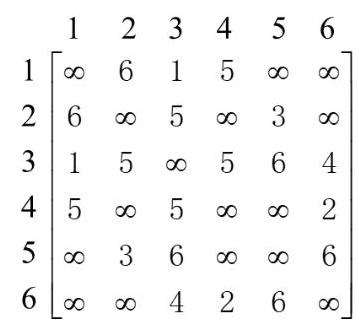
\includegraphics[width=0.3\textwidth]{images/2021/comprehensive_31.jpg}
\end{center}
\hspace*{3em} 

(1)求从顶点 1 出发的广度优先搜索序列；

(2)根据 prim 算法,求图 \(G\) 从顶点 1 出发的最小生成树, 要求表示出其每一步生成过程。
\vspace{10em}

\newpage
32 (10 分) 表 32-1 中,第 0 行是待排序序列的原始输入(12 2 16 30 28 10 16*20 6 18); 其他各行是 5 种排序算法得到的某个中间步骤的内容。表 32-2 列出了 6 种排序算法。请按行序直接给出每行对应排序算法的编号。每个编号只使用一次。

表 32- 排序算法 序列

\begin{center}
\begin{tabular}{|c|c|c|c|c|c|c|c|c|c|c|}
\hline
第 0 行 & 原始输入 & 12 & 2 & 16 & 30 & 28 & 10 & 16* & 20 & 6 \\
\cline{1-11}
算法 & \phantom{X} & 2 & 12 & 16 & 30 & 28 & 10 & 16* & 20 & 6 \\
\cline{1-11}
算法 & \phantom{X} & 6 & 2 & 10 & 12 & 28 & 30 & 16* & 20 & 16 \\
\cline{1-11}
\hline
\end{tabular}
\end{center}

\begin{center}
\begin{tabular}{|c|c|c|c|c|c|c|c|c|c|c|}
\hline
算 法 & \phantom{X} & 2 & 12 & 16 & 30 & 10 & 28 & 16* & 20 & 6 \\
\cline{1-11}
算法 & \phantom{X} & 10 & 2 & 16 & 6 & 18 & 12 & 16* & 20 & 30 \\
\cline{1-11}
算法 & \phantom{X} & 2 & 12 & 16 & 28 & 10 & 16* & 20 & 6 & 18 \\
\cline{1-11}
\hline
\end{tabular}
\end{center}

表 32-2:

\begin{center}
\begin{tabular}{|c|c|}
\hline
排序算法 编号 & 排序算法名称 \\
\cline{1-2}
A & 希尔排序(增量 为 \(5,2,1)\) \\
\cline{1-2}
B & 快速排序 \\
\cline{1-2}
C & 直接选择排序 \\
\cline{1-2}
\hline
\end{tabular}
\end{center}

\begin{center}
\begin{tabular}{|c|c|}
\hline
排序算法 编号 & 排序算法名称 \\
\cline{1-2}
D & 二路归并排序 \\
\cline{1-2}
E & 直接插入排序 \\
\cline{1-2}
F & 冒泡排序 \\
\cline{1-2}
\hline
\end{tabular}
\end{center}
\vspace{10em}

\section*{四、算法分析与设计题(本大题共 2 小题, 每小题 15 分, 共 30 分)}

33 如果一个序列是一个先单调递增后单调递减的序列, 那么它称为双调序列。设计一个尽可能高效的算法,找到由 \(\mathrm{N}\) 个数组成的一个双调序列中最大的关键值。要求:

(1)描述算法的基本设计思想；

(2)根据设计思想,采用 \(\mathrm{C}\) 或 \(\mathrm{C} +  +\) 语言描述算法,关键之处给出注释;

(3)说明你所设计的算法的时间复杂度和空间复杂度。
\vspace{15em}

34 设有一个正整数序列组成的有序单链表 (按递增有序, 且允许有相等的整数存在), 请设计一个用最小的时间和最小空间的算法实现下列功能:(a) 确定在序列中比正整数 \(x\) 大的数有几个 (相同的数只计算一次,如序列 \(\{ 3\text{ 、 }5\text{ 、 }6\text{ 、 }6\text{ 、 }8\text{ 、 }{10}\text{ 、 }{11}\text{ 、 }{13}\text{ 、 }{13}\) 、 \({16}\text{ 、 }{17}\text{ 、 }{20}\text{ 、 }{20}\}\) 中比 10 大的数有 5 个); (b) 将单链表中比正整数 \(x\) 小的数按递减次序排列；(c) 将正整数比 \(x\) 大的偶数从单链表中删除。要求:

(1)描述算法的基本设计思想；

(2)根据设计思想,采用 \(\mathrm{C}\) 或 \(\mathrm{C} +  +\) 语言描述算法,给出注释；

(3)说明你所设计的算法的时间复杂度和空间复杂度。



提示: 节点定义供参考 提示: 算法定义形式供参考

\begin{lstlisting}[language=C, basicstyle=\ttfamily]
typedef struct node {
    int data;
    struct node *next;
}LNode,*LinkList;
\end{lstlisting}

\begin{lstlisting}[language=C, basicstyle=\ttfamily]
void FunctionExam(LinkList L1, int x) 
{
    ......
}
\end{lstlisting}



\newpage

\chapter{2022}

\section*{一、 选择题 (本大题共 15 小题, 每小题 2 分, 共 30 分)}

1. 当输入非法错误时,一个“好”的算法会进行适当处理,而不会产生难以理解的输出结果。 这称为算法的(   )。

A. 可读性 B. 健壮性 C. 正确性 D. 有穷性

2. 当字符序列 F4\_作为一个栈的输入时,输出长度为 3 的且可用作 C 语言标识符的序列有(   )个。

A. 4 B. 5 C. 3 D. 6

3. 若用一个大小为 7 的数组来实现循环队列, 且当前 rear 和 front 的值分别为 0 和 4 , 当从队列中删除一个元素,再加入两个元素后, rear 和 front 的值分别为(   )。

A. 2 和 6 B. 6 和 2 C. 5 和 2 D. 2 和 5

4. 用一个栈求下列后缀表达式的值,
\begin{center}
    \verb|8 2 3 ^ / 2 3 * + 5 1 * -|
\end{center}

其中:+、-、*、/、\^分别是加、减、乘、除、幂运算符,当扫描到第一个*时,栈顶部 2 个元素是(   )。

A.6,1 B.5,7 C.3,2 D.1,5

5. 某二叉树的前序序列和后序序列正好相反,则该二叉树一定是(   )的二叉树。

A. 空或只有一个节点 B. 高度等于其节点数

C. 任一节点无左孩子 D. 任一节点无右孩子

6. 一棵左子树为空的二叉树在前序线索化后,其中空的链域的个数是(   )。

A. 不确定 B. 0 C. 1 D. 2

7. (   ) 占用的额外空间的空间复杂性为 \(O\left( 1\right)\) 。

A. 堆排序算法 B. 归并排序算法

C. 快速排序算法 D. 以上答案都不对

8. 在 Huffman 编码中, 若编码长度只允许小于等于 3 , 则除了已对两个字符编码为 0 和 10 外,还可以最多对(   )个字符编码。

A. 2 B. 3 C. 4 D. 5

9. 设一个稀疏矩阵有 1000 行 850 列, 其中有 800 个非 0 元素。设每个整数占 \(2\mathrm{\;B}\) , 数据值占 4B,则用三元组表存储该矩阵时所需字节数是(   )。

A. 1600 B. 3200 C. 6400 D. 9600

10. 用于求无向图的所有连通分量的算法是(   )。

A. 广度优先遍历 B. 拓扑排序 C. 求最短路径 D. 求关键路径

11. 若需在 \(O\left( {n{\log }_{2}n}\right)\) 的时间内完成对数组的排序,且要求排序是稳定的,则可选择的排序方法是(   )。

A. 快速排序 B. 堆排序 C. 归并排序 D. 直接插入排序

12. 下列(   )的邻接矩阵是对称矩阵。

A. AOV 网 B. AOE 网 C. 有向图 D. 无向图

13. 将元素 71、65、84、69、67、83 逐个插入空的二叉排序树(BST)中,最低层的元素为 (   )。

A. 65 B. 67 C. 69 D. 83

14. 具有 12 个关键字的有序表,折半查找的平均查找长度为(   )。

A. 3.1 B. 4 C. 2.5 D. 5

15. 若在一棵 \(m\) 阶 \(\mathrm{B}\) 树的结点中插入新关键码后该结点必须分裂为两个结点,那么在插入前结点的关键码数应为(   )。

A. \(m\) B. \(m - 1\) C. \(m + 1\) D. \(m - 2\)

\section*{二、填空题(本大题共 10 小题,每小题 3 分,共 30 分)}

16. 对于具有 144 个记录的文件, 若采用分块查找法, 且每块长度为 8 , 采用顺序查找确定所在的块,则平均查找长度为(   )。

17. A、B、C、D、E、F和G这七个元素以相反的顺序被压入堆栈，即从G开始。堆栈被弹出五次，每个元素被插入到队列中。从队列中删除两个元素并将其推回到堆栈中。现在，一个元素被弹出从堆栈中。弹出的项是(   ).

18. 有 \(n\) 个字符的字符串的非空子串个数最多有(   )个。

19. 用有向无环图描述表达式 \({\left( a + b\right) }^{ * }\left( {\left( {a + b}\right) /a}\right)\) ,至少需要顶点的数目为(   )。

20. 由 3 个结点可以构造出(   )种不同的二叉树。

21. 若一个具有 \(n\) 个顶点, \(e\) 条边的无向图是一个森林,则该森林中必有(   )棵树。

22. 对于长度为 18 的有序顺序表, 若采用折半查找, 则查找第 15 个元素的查找次数为 (   )。

23. (   )是哈希表的一个重要参数,它反映哈希表的装 满程度。

24. 硬件厂商 XYZ 公司宣称他们最新研制的微处理器运行速度为其竞争对手 ABC 公司同类产品的 100 倍。对于计算复杂度为 \({n}^{2}\) 的算法,若用 \(\mathrm{{ABC}}\) 公司的计算机能在 1 小时内解输入规模为 \(n\) 的问题,那么用 XYZ 公司的计算机在 1 小时内能解输入规模为 (   ) 的问题。

25. 表达式 \(A/B + D\$ E + F/H\) 中,运算符的优先级由高到低依次为 \(+ ,/,\$\) ,均右结合,则相应的后缀式是 (   )。

\section*{三、 综合应用题 (本大题共 7 小题, 共 60 分)}

26. (5 分) 阅读代码, 函数 print(   )接收 二叉查找树/二叉排序树(BST)的根和 一个正整数 \(k\) 作为参数。请:

// a BST node
\begin{lstlisting}[language=C, basicstyle=\ttfamily]
struct node { 
    int data;
    struct node *left, *right;
};
int count = 0;
void print(struct node *root, int k)
{
    if(root != NULL&&count<=k)
    {
        print(root->right, k);
        count++;
        if(count==k)
            printf("%d", root->data);
        print(root->left, k);
    }
}
\end{lstlisting}

(1)简述该代码的功能；

(2)print(root, 3)的输出是什么?其中 root 表示下图 BST 树的根。

\begin{center}
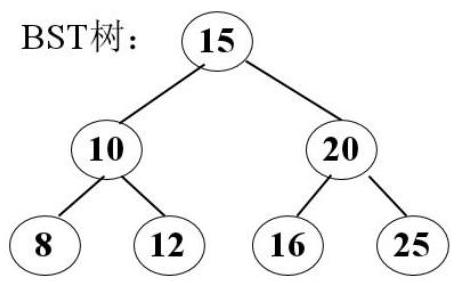
\includegraphics[width=0.3\textwidth]{images/2022/comprehensive_26.jpg}
\end{center}
\vspace{10em}

27. (5 分) 有一段代码:
\begin{lstlisting}[language=C, basicstyle=\ttfamily]
int count = 0;
for (int i=0;i<N;++)
    for (int j=i+1;j<N;j++)
        for (int k=j+1;k<N;k++)
            if (a[i]+a[j]>=a[k])count++;
\end{lstlisting}

假设 \(\mathrm{N} = {1000}\) 时,执行这段代码需要 1 秒时间。现在对这段代码的运行时间 (秒) 进行预估,请用一个关于 \(N\) 的函数来表示。
\vspace{10em}

\newpage
28. (10分)设 \(\mathrm{A},\mathrm{B},\mathrm{C},\mathrm{D},\mathrm{E}\) 五个字符的编码分别为1,2,3,4,5,并设标识符按以下次序出现: AA, BB, BD, BE, AB, AD, CD, BC, AE, DD。要求用哈希 (Hash) 方法将它们存入具有 10 个位置的表中。

(1)将上述关键字(标识符)构造一个哈希函数, 使得发生冲突尽可能地少;

(2)采用线性探测再散列法解决冲突, 写出上述各关键字在表中的位置, 并给出比较次数；即:填写完整下表。
\begin{center}
\begin{tabular}{|c|c|c|c|c|c|c|c|c|c|c|}
\hline
哈希地址 & 0 & 1 & 2 & 3 & 4 & 5 & 6 & 7 & 8 & 9 \\
\cline{1-11}
关键字 & \phantom{X} & \phantom{X} & \phantom{X} & \phantom{X} & \phantom{X} & \phantom{X} & \phantom{X} & \phantom{X} & \phantom{X} & \phantom{X} \\
\cline{1-11}
比较次数 & \phantom{X} & \phantom{X} & \phantom{X} & \phantom{X} & \phantom{X} & \phantom{X} & \phantom{X} & \phantom{X} & \phantom{X} & \phantom{X} \\
\cline{1-11}
\hline
\end{tabular}
\end{center}
\vspace{15em}

29. (10分)已知一棵二叉查找树/二叉排序树(BST)的先序遍历序列为30,20,10,15, 25,23,39,35,42。

(1)请画出此二叉树的形态。

(2)请给出这棵树的后序遍历序列。

(3)画出此二叉树的中序线索二叉树。

(4)画出与此二叉树对应的森林。
\vspace{10em}

\newpage
30. (12 分) 已知图 \(G\) 如右边所示:

\begin{figure}[htbp]
    \centering
    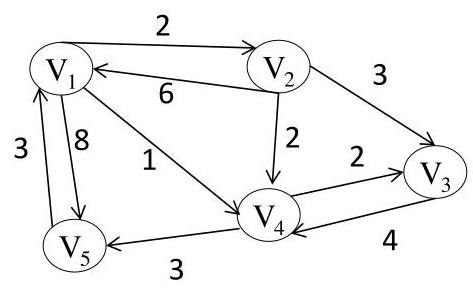
\includegraphics[width=0.3\textwidth]{images/2022/comprehensive_30.jpg}
    \caption*{图G} % 使用带星号的 caption*
\end{figure}
(1)画出 \(G\) 的邻接表表示图；

(2)根据你画的邻接表,以顶点 \({V}_{1}\) 为根,画出 \(G\) 的深度优先生成树;

(3)利用弗洛伊德算法(Floyd)求每一对顶点之间的最短路径, 请给出带权长度矩阵

\({\mathbf{D}}^{\left( 0\right) },{\mathbf{D}}^{\left( 1\right) }\) 和 \({\mathbf{D}}^{\left( 2\right) }\) 。
\vspace{10em}

31. (8分)考虑序列:‘mississippi’,请:

(1)采用赫夫曼(Huffman)编码算法对上述序列编码, 给出相应的 Huffman 树, 以及每个字符的 Huffman 码。 

(2)一共需要多少 bit 位?
\vspace{10em}

\newpage
32. (10 分)下表 32-1 中第 0 行是待排序序列的原始输入(Eagle Ant Dog Frog Cat Horse Bee Goat); 其他各行是 5 种排序算法得到的某个中间步骤的内容。 表 32-2 列出了 6 种排序算法。

请按行序直接给出每行对应排序算法的编号。每个编号只使用一次。

表 32-1: 行号 排序算法 序列

\begin{table}[htbp]
\centering
\caption{表 32-1}
\begin{tabular}{lll}
\toprule
行号 & 排序算法 & 序列 \\
\midrule
\textbf{第0行} & \textbf{原始输入} & \textbf{Eagle Ant Dog Frog Cat Horse Bee Goat} \\
\midrule
& 算法 1: & Ant Dog Eagle Frog Cat Horse Bee Goat \\
& 算法 2: & Ant Dog Eagle Frog Bee Cat Goat Horse \\
& 算法 3: & Ant Bee Dog Frog Cat Horse Eagle Goat \\
& 算法 4: & Bee Ant Dog Eagle Cat Horse Frog Goat \\
& 算法 5: & Bee Ant Dog Cat Eagle Horse Frog Goat \\
\bottomrule
\end{tabular}
\end{table}

\begin{center}
\begin{tabular}{|c|c|c|c|c|c|c|c|c|c|}
\hline
算法 3: & \phantom{X} & Ant & Bee & Dog & Frog & Cat & Horse & Eagle & Goat \\
\cline{1-10}
算法 4: & \phantom{X} & Bee & Ant & Dog & Eagle & Cat & Horse & Frog & Goat \\
\cline{1-10}
算法 5: & \phantom{X} & Bee & Ant & Dog & Cat & Eagle & Horse & Frog & Goat \\
\cline{1-10}
\hline
\end{tabular}
\end{center}

表 32-2:

\begin{center}
\begin{tabular}{|c|c|}
\hline
排序算法编号 & 排序算法名称 \\
\cline{1-2}
A & 冒泡排序 \\
\cline{1-2}
B & 直接插入排序 \\
\cline{1-2}
C & 希尔排序(增量为 3, 1) \\
\cline{1-2}
D & 快速排序 \\
\cline{1-2}
E & 简单选择排序 \\
\cline{1-2}
F & 二路归并排序 \\
\cline{1-2}
\hline
\end{tabular}

\end{center}
\vspace{20em}

\section*{四、算法分析与设计题 (本大题共 2 小题, 共 30 分)}

33. (15 分)设计一个算法,将一个用循环链表表示的稀疏多项式分解成两个多项式,使这两个多项式中各自仅含奇次项或偶次项, 并要求利用原链表中的结点空间构成这两个链表。要求:

(1)描述算法的基本设计思想；

(2)根据设计思想,采用 \(\mathrm{C}\) 或 \(\mathrm{C} +  +\) 语言描述算法,关键之处给出注释；

(3)说明所设计算法的时间复杂度和空间复杂度。
\vspace{6em}

提示: 其中稀疏多项式采用的循环链表存储结构 LinkedPoly 定义为
\begin{lstlisting}[language=C, basicstyle=\ttfamily]
typedef struct PolyNode {
    float coef; //单项式的系数
    int exp; //单项式的指数
    struct PolyNode *next;
}PolyNode;
typedef PolyNode*LinkedPoly;
\end{lstlisting}

算法描述,只需要给出如何将循环链表 \(\mathrm{L}\) 分成满足要求的两个循环链表的操作,即完善下述函数: 
\begin{lstlisting}[language=C, basicstyle=\ttfamily]
void Divide (LinkedPoly L) {
......
}
\end{lstlisting}
\vspace{20em}


34. (15分) 从根到叶子的最大距离称为树的半径。给定一个无向连通图,写一个算法找出半径最小的生成树。要求:

(1)描述算法的基本设计思想；

(2)根据设计思想,采用 \(\mathrm{C}\) 或 \(\mathrm{C} +  +\) 语言描述算法,关键之处给出注释；

(3)说明所设计算法的时间复杂度和空间复杂度。
\newpage

\chapter{2023}
\section*{一. 程序阅读题(本大题共 4 小题,共 20 分)}

1. (4 分) 有一段代码:
\begin{lstlisting}[language=C, basicstyle=\ttfamily]
int brute(int a[], int N) {
    int i,j,k,m;
    for(i=0;i<N;i++)
        for(j=i+1;j<N;j++)
            for(k=j+1;k<N;k++)
                for(m=k+1;m<N;m++)
                    if(a[i]+a[j]+a[k]+a[m] == 0) return 1;
    return 0;
}
\end{lstlisting}

假设 \(N = {1000}\) 时,执行这段代码需要 1000 秒时间。当 \(N = {10000}\) 时,请预测它的运行时间是多少秒。
\vspace{5em}

2. (5分) 有如下代码段:
\begin{lstlisting}[language=C, basicstyle=\ttfamily]
int mystery(int m int n) {
    int p = 1;
    int x = m;
    int y = n;
    while (y!=0){
        if(y%2==0){x*=x;y/=2;}
        else {y-=1;p*=x;}
    }
    return p
}
\end{lstlisting}




(1) \(m,n\) 是两个整数, \(m,n \geq  0\) ,请问函数 \({mystery}\left( {m,n}\right)\) 的功能是什么？

(2)给出在最坏情况下,这段代码的时间复杂度,用 \(n\) 的函数表示。
\vspace{5em}

3.(5分)一个单链表按序存放一个整数序列 \(\{ 1,2,3,4,5,6,7\}\) ,且该单链表作为函数rearrange的输入。请写出执行函数rearrange后的输出。
\vspace{10em}

\begin{lstlisting}[language=C, basicstyle=\ttfamily]
struct node {
    int value;
    struct node *next;
};
void rearrange(struct node *list) {
    struct node *p, *q;
    int temp;
    if((!list)||!list->next)
        return;
    p = list;
    q = list->next;
    while(q) {
        temp = p->value;
        p->value = q->value;
        q->value = temp;
        p = q->next;
        q = p ? p->next : 0;
    }
}
\end{lstlisting}
\vspace{8em}

4. (6 分) 下列代码交换双向链表中两个相邻的元素。请填写完整代码。

双向链表存储结构:

\begin{lstlisting}[language=C, basicstyle=\ttfamily]
struct DLinkNode {
    ElementType data;
    Position prior; //Front pointer
    Position next; //Rear pointer
};
struct DLinkNode;
typedef struct DLinkNode *PtrToNode;
typedef struct PtrToNode DLinkList;
typedef struct PtrToNode Position;
void SwapWithNext( Position P, DLinkList L ) {
    Position BeforeP, AfterP;
    BeforeP = P->prior;
    AfterP = P->next;
    P->next = AfterP->next;
    __________(1)___________;
    AfterP->next = P;
    __________(2)___________;
    __________(3)___________;
    AfterP->prior = BeforeP;
}
\end{lstlisting}



\section*{二. 填空题 (本大题共 10 小题, 每小题 3 分, 共 30 分)}

5. 有 5 个元素, 其入栈次序为: A, B, C, D, E, 在各种可能的出栈次序中, 以元素 \(\mathrm{C}\) 、 \(\mathrm{D}\) 最先出栈(即 \(\mathrm{C}\) 第一个且 \(\mathrm{D}\) 第二个出栈)的次序有\_\_\_\_\_\_\_\_个。

6. 假设栈初始为空,在将中缀表达式 \({\left( a + b/c\right) }^{ * }\left( {d - {e/f}}\right)\) 转换为等价的后缀表达式的过程中,当扫描到‘e’时,栈中的元素从栈底开始依次是\_\_\_\_\_\_\_\_。

7. 若用一个大小为 8 的数组来实现循环队列, 且当前 rear 和 front 的值分别为 0 和 3 , 当从队列中删除两个元素, 再加入三个元素后, front 的值为\_\_\_\_\_\_\_\_。

8. 有一个 \(8 * 8\) 的对称矩阵 \(M\) 的上三角部分的元素 \({m}_{\mathrm{i},\mathrm{j}}\left( {1 \leq  i \leq  j \leq  8}\right)\) 按行优先存入 \(\mathrm{C}\) 语言的一维数组 \(N\) 中,元素 \({m}_{6,4}\) 在 \(N\) 中的下标是\_\_\_\_\_\_\_\_。

9. 在一棵度为 4 的树 T 中,若有 18 个度为 4 的结点, 10 个度为 3 的结点, 6 个度为 2 的结点,6 个度为 1 的结点,则树T 的叶子结点个数是\_\_\_\_\_\_\_\_。

10. 在图 1 所示的平衡二叉树中插入关键字 46 后得到一棵新的平衡二叉树, 在新的平衡二叉树中, 关键字 35 所在结点的左孩子结点中保存的关键字是\_\_\_\_\_\_\_\_。

\begin{figure}[htbp]
    \centering
    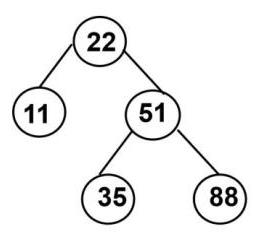
\includegraphics[width=0.3\textwidth]{images/2023/blank_10.jpg}
    \caption*{图1 10题图} % 使用带星号的 caption*
\end{figure}

11. 在有序表 A[1..11]中, 采用折半查找算法查等于 A[8]的元素, 所比较的元素下标依次为\_\_\_\_\_\_\_\_。

12. 已知待排序的 \(n\) 个元素可分为 \(n/k\) 个组,每个组包含 \(k\) 个元素,且任一组内的各元素均分别大于前一组内的所有元素和小于后一组内的所有元素,若采用基于比较的排序,其时间下界为\_\_\_\_\_\_\_\_。

13. 对 \(n\) 个记录的文件进行堆排序,最坏情况下的执行时间下界是\_\_\_\_\_\_\_\_。

14. 在含有 \(n\) 个结点的三叉链表中有\_\_\_\_\_\_\_\_个空链域。

\section*{三. 综合应用题 (本大题共 8 小题, 共 70 分)}

15.(6分)设一个有向图 \(G = \left( {V,E}\right)\) ,其中:

\(V = \left\{  {{v}_{1},{v}_{2},{v}_{3},{v}_{4},{v}_{5}}\right\}  ,\)

\(\left. {E = \left\{  { < {v}_{1},{v}_{5} > , < {v}_{1},{v}_{2} > , < {v}_{1},{v}_{3} > , < {v}_{2},{v}_{3} > , < {v}_{3},{v}_{4} > , < {v}_{5},{v}_{4} > }\right\}  }\right\}\)

给出其所有的拓扑序列。
\vspace{10em}

16. ( 3 分) 画出一个二叉树,使得它既满足大根堆的要求,又满足二叉查找树的要求。

\begin{figure}[htbp]
    \centering
    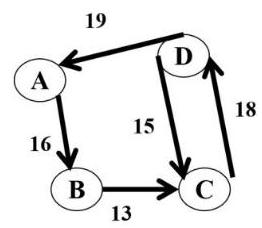
\includegraphics[width=0.3\textwidth]{images/2023/comprehensive_16.jpg}
    \caption*{图2 17题图} % 使用带星号的 caption*
\end{figure}
\vspace{10em}

\newpage
17. (8 分) 一个有向图 \(G\) 如图 2 所示: 使用单源点最短路径算法 Dijkstra 求解图 \(G\) 中 \(\mathrm{A}\) 点到其他各点的最短路径, 要求给出计算过程。
\vspace{10em}

18.(13分)图 3 是一个有三棵树的森林。

(1)采用二叉链表(孩子兄弟表示法)来存储森林,画出该森林对应的二叉树;

(2)画出上述二叉树的后序线索树；

(3)用先序和中序分别遍历该森林,写出遍历后的结点序列。

\begin{figure}[htbp]
    \centering
    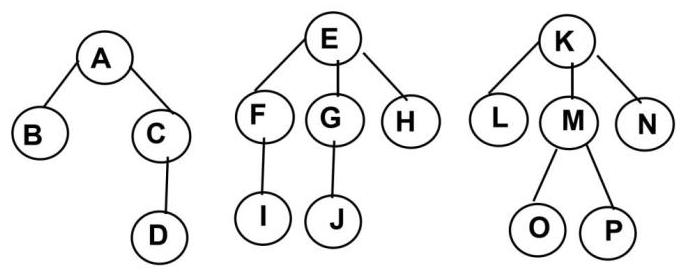
\includegraphics[width=0.3\textwidth]{images/2023/comprehensive_18.jpg}
    \caption*{图3 18题图} % 使用带星号的 caption*
\end{figure}
\vspace{10em}

\newpage
19. (7 分) 设散列表为 \({HT}\left\lbrack  {0.{.9}}\right\rbrack\) ,即表的大小为 \(m = {10}\) 。现采用双散列法解决冲突。散列函数和再哈希函数分别为:

\({h}_{1}\left( x\right)  = x{\;\operatorname{mod}\;{10}},\)

\({h}_{2}\left( x\right)  = 7 - \left( {x{\;\operatorname{mod}\;7}}\right)\) 。

若插入的关键码序列为(4371, 1323, 6173, 4199, 4344, 9679, 1989),写出上述各关键字在表中的位置。(即:填写完整如下所示表格。)

\begin{center}
\begin{tabular}{|c|c|c|c|c|c|c|c|c|c|c|}
\hline
哈希地址 & 0 & 1 & 2 & 3 & 4 & 5 & 6 & 7 & 8 & 9 \\
\cline{1-11}
关键字 & \phantom{X} & \phantom{X} & \phantom{X} & \phantom{X} & \phantom{X} & \phantom{X} & \phantom{X} & \phantom{X} & \phantom{X} & \phantom{X} \\
\cline{1-11}
\hline
\end{tabular}
\end{center}

\vspace{5em}

20. (10分)设某通信信息由 a, b, c, d, e, f 这 6 个字母组成,每个字母出现的次数分别为 5, 9, 12, 13, 16, 45。每个字母在信息传输时需要 1Byte(字节) 的空间。现在将这个信息采用赫夫曼(Huffman)算法压缩成二进制 0,1 序列传输。请问:

(1)压缩后的信息将节约多少 bits(位)？

(2)画出这里设计的 Huffman 树。
\vspace{10em}

\newpage
21. ( 13 分)已知图 G 如图 4 所示:

\begin{figure}[htbp]
    \centering
    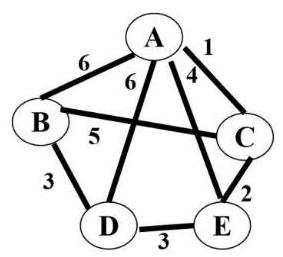
\includegraphics[width=0.3\textwidth]{images/2023/comprehensive_21.jpg}
    \caption*{图4 21题图} % 使用带星号的 caption*
\end{figure}

(1)画出 G 的邻接表表示图；

(2)根据你画的邻接表,以顶点 \(\mathrm{A}\) 为根, 画出 \(G\) 的深度优先生成树;

(3)根据普里姆(Prim)算法,求图 \(\mathrm{G}\) 从顶点 \(\mathrm{A}\) 出发的最小生成树,要求表示出其每一步生成过程。
\vspace{10em}

22. (10分)设一数组中有数据:5,1,4,6,3,8,2,7。写出用下列排序算法进行一遍排序后的结果。

(1) 冒泡排序 (2)直接插入排序 (3) 快速排序

(4) 简单选择排序 (5) 二路归并排序
\vspace{10em}

\section*{四. 算法设计与分析题 (本大题共 2 小题, 共 30 分)}

23. (15分)已知 \(L\) 为链表的头结点地址,表中共有 \(m\left( {m > 3}\right)\) 个结点,从表中第 \(i\left( {1 < i < m}\right)\) 个结点起到第 \(m\) 个结点构成一个循环部分链表。试设计一时间复杂度 \(\mathrm{O}\left( n\right)\) 的算法 PatternInvert \(\mathrm{L}\left( {\text{ LinkList }L\text{ , int }i\text{ , int }m}\right)\) ,将这部分循环链表中所有结点顺序完全倒置。要求:

(1)描述算法的基本设计思想；

(2)根据设计思想,采用 \(\mathrm{C}\) 语言描述算法,关键之处给出注释。

\begin{figure}[htbp]
    \centering
    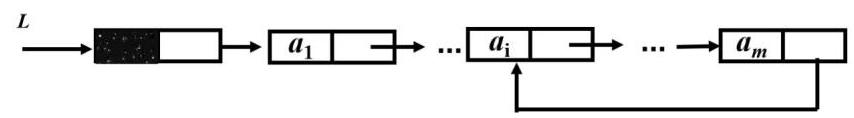
\includegraphics[width=0.3\textwidth]{images/2023/algorithm_23.jpg}
    \caption*{图4 21题图} % 使用带星号的 caption*
\end{figure}

结点定义如下:



typedef struct node

\{

\hspace*{1em} int data;

\hspace*{1em} struct node *next;

\}LNode,*LinkList;
\vspace{13em}

24. (15分)给定一个 \({nm}\) 的矩形位图,位图中的每个像素不是白色就是黑色,但至少有一个是白色的。第 \(i\) 行第 \(j\) 列的像素被称作像素(i, j)。两个像素 \({p}_{1} = \left( {{i}_{1},{j}_{1}}\right) ,{p}_{2} = \left( {{i}_{2},{j}_{2}}\right)\) 之间的距离定义为: \(d\left( {{p}_{1},{p}_{2}}\right)  = \left| {{i}_{1} - {i}_{2}}\right|  + \left| {{j}_{1} - {j}_{2}}\right|\) 。现在请设计一个时间复杂度尽可能低的算法来计算图中每个像素与离其最近的“白像素”的距离。

输入: 第 1 行包含两个整数 \(n\) 和 \(m\left( {1 \leq  n \leq  {150},1 \leq  m \leq  {150}}\right)\) ,用一个空格隔开。 接下来 \(n\) 行,每一行都包含一个长度为 \(m\) 的 01 串。第 \(i + 1\) 行第 \(j\) 列的字符若为 1 ,则像素(i, j)是白色的；否则是黑色的。

输出: 包含 \(n\) 行,每行有 \(m\) 个用空格隔开的整数。第 \(i\) 行第 \(j\) 列的整数表示(i, j)与离其最近的白像素之间的距离。

要求:

(1)描述算法的基本设计思想；

(2)根据设计思想,采用类 \(\mathrm{C}\) 语言的伪代码描述算法,关键之处给出注释。

( 3 )说明你所设计的算法的时间复杂度。

\newpage

\chapter{2024}
\section*{一、程序阅读题}

1. 有一个整数 n, 其中 n 为 2 的幂。程序通过如下代码计算 count 的值, 并返回。请分析并给出该代码的时间复杂度。

\begin{lstlisting}[language=C, basicstyle=\ttfamily]
int main() {
    int count = 0;
    int x = 2;
    while (x < n/2) {
        x = x * 2;
        count++;
    }
    return count;
}
\end{lstlisting}

2. 下面给出一段关于链表操作的代码片段, 请将这些代码片段按正确的顺序排列, 使其实现将结点 \(\mathrm{s}\) 插入到结点 \(\mathrm{p}\) 之前的功能(假设 \(\mathrm{p}\) 既不是头结点也不是尾结点),并分析时间复杂度。代码片段如下:

① prev->next != p \&\& prev->next != NULL

② prev->next = s

③ head == NULL || p == NULL || s == NULL

④ prev->next == p
\begin{lstlisting}[language=C, basicstyle=\ttfamily]
void insertBefore(Node* head, Node* p, Node* s){
    if (______) return;
    Node* prev = head;
    while (______) {
        prev = prev->next;
    }
    if (______) {
        s->next = p;
        ______
    }
}
\end{lstlisting}

\newpage

3. 合并两个非递减的链表为一个非递增链表,以下是部分代码, 请补全代码使其正确实现功能,假设链表的长度分别为 \(\mathrm{n}\) 和 \(\mathrm{m}\) ,分析这段代码的时间复杂度。

\begin{center}
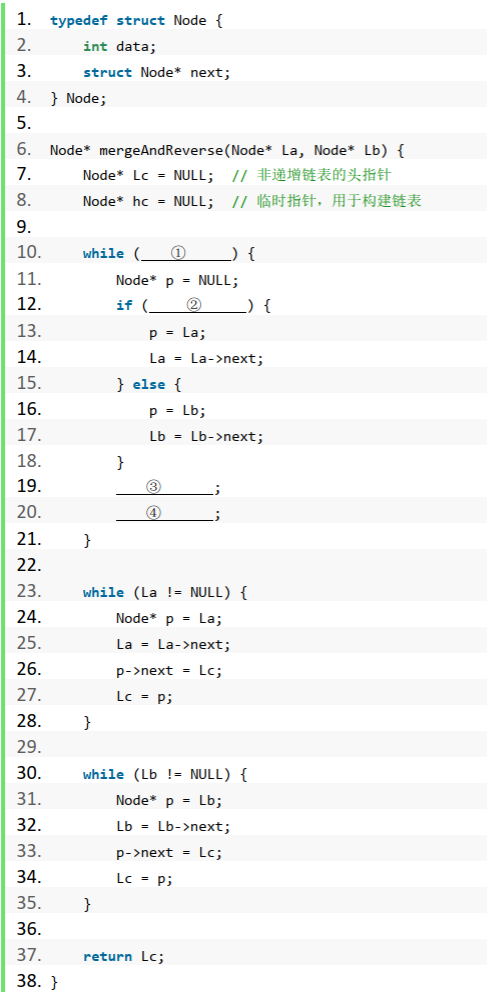
\includegraphics[width=0.6\textwidth]{images/2024/3.png}
\end{center}

4. 请补全下面拓扑排序算法中的代码,假设顶点数为 \(\left| V\right|\) ,边数为 \(\left| E\right|\) ,分析这段代码的时间复杂度。

\begin{lstlisting}[language=C, basicstyle=\ttfamily]
bool Topologicalsort(Graph G) {
    InitStack(S);
    for (int i = 0; i < G.vexnum; i++) {
        if (indegree[i] == 0) {
            ______①______;
        }
    }
    int count = 0;
    while (______②______) {
        ______③______;
        print[count++] = i;
        for (p = G.vertices[i].firstarc; ______④______; p = p->nextarc) {
            v = p->adjvex;
            if (!(--indegree[v])) {
                Push(S, v);
            }
        }
    }
    if (count < G.vexnum) {
        return false;
    } else {
        return true;
    }
}
\end{lstlisting}

\newpage

5. 描述以下递归代码的功能。

\begin{lstlisting}[language=C, basicstyle=\ttfamily]
int func(TreeNode* root) {
    if (root == NULL) {
        return 0;
    }
    if (root->left == NULL && root->right == NULL) {
        return 1;
    }
    return func(root->left) + func(root->right);
}
\end{lstlisting}

\section*{二、填空题}

1. 设循环队列的表长为 \(\mathrm{n},\mathrm{f}\) 指向元素的前一个位置, \(\mathrm{r}\) 指向最后一个元素的位置。该循环队列的长度为\_\_\_\_\_。

2. 将中缀表达式 a+b-a*((c+d)/e-f)+g 转换为后缀表达式\_\_\_\_\_。

3. 给定字符串 abcaabbabcab, 求其对应的 next 数组。

\begin{center}
\begin{tabular}{|c|c|c|c|c|c|c|c|c|c|c|c|c|}
\hline
\phantom{X} & \(\mathbf{a}\) & b & c & a & a & b & b & a & b & c & a & b \\
\cline{1-13}
下标 i & 1 & 2 & 3 & 4 & 5 & 6 & 7 & 8 & 9 & 10 & 11 & 12 \\
\cline{1-13}
next[i] & \phantom{X} & \phantom{X} & \phantom{X} & \phantom{X} & \phantom{X} & \phantom{X} & \phantom{X} & \phantom{X} & \phantom{X} & \phantom{X} & \phantom{X} & \phantom{X} \\
\cline{1-13}
\hline
\end{tabular}
\end{center}

4. 在哈夫曼树中,已知有 1247 个结点,叶子结点的个数为\_\_\_\_\_。

5. 对序列 \(\{ 1,2,3,4,5,6,7\}\) 进行顺序插入构建平衡二叉树,平衡因子为 0 的结点个数为\_\_\_\_\_。

6. 给定一个二维数组 \(\mathrm{A}\left\lbrack  {10}\right\rbrack  \left\lbrack  {15}\right\rbrack  ,\mathrm{A}\left\lbrack  0\right\rbrack  \left\lbrack  0\right\rbrack\) 的地址为 644,行优先存储,每个元素占用一个地址空间, A[4][5]的地址为\_\_\_\_\_。

7. 已知一棵树有 2011 个结点, 其中 116 个是叶结点, 其对应二叉树中右子树为空的结点数量为\_\_\_\_\_。

8. 设森林 F 中有三棵树,第一,第二,第三棵树的结点个数分别为 M1、M2 和 M3。 与森林 F 对应的二叉树根结点的左子树上的结点个数是\_\_\_\_\_。

9. 已知一棵完全二叉树的第六层有 8 个叶结点, 树根位于第一层, 树的最多结点数为\_\_\_\_\_。

\section*{三、综合应用题}

1. 设数组 \(\mathrm{S}\left\lbrack  \right\rbrack   = \{ {93},{946},{372},9,{146},{151},{301},{485},{236},{372},{43},{892}\}\) , (1)采用最低位优先(LSD)基数排序将 S 排列成升序序列。写出每一趟排序的结果。

(2)增量等于 5 时进行希尔排序,写出第一趟排序结果。

(3)以第一个元素为轴进行快速排序,写出第一趟排序结果。

(4)构造小根堆,写出调整后的小根堆。

2. 设散列函数 \(\mathrm{H}\left( \mathrm{{key}}\right)  = \mathrm{{key}}\;\mathrm{MOD}\;{11}\) ,用线性探测再散列法解决冲突。对关键字序列 (13,28,72,5,16,18,7,11,24) 在地址空间为 0-10 的散列区中建散列表, 画出此表, 并求等概率情况下查找成功和查找失败时的平均查找长度。

\begin{center}
\begin{tabular}{|c|c|c|c|c|c|c|c|c|c|c|c|}
\hline
下标 & 0 & 1 & 2 & 3 & 4 & 5 & 6 & 7 & 8 & 9 & 10 \\
\cline{1-12}
关键字 & \phantom{X} & \phantom{X} & \phantom{X} & \phantom{X} & \phantom{X} & \phantom{X} & \phantom{X} & \phantom{X} & \phantom{X} & \phantom{X} & \phantom{X} \\
\cline{1-12}
\hline
\end{tabular}
\end{center}

\newpage
3. 一棵二叉树的先序、中序和后序序列如下, 其中有部分未标出:

先序序列:\_\_\_\_\_ \(\mathrm{{CDE}}\_ \mathrm{{GHI}}\_ \mathrm{K}\)

中序序列:CB \_ FA \_ J K I G

后序序列: \_ \(\mathrm{{EFDB}}\) \_ \(\mathrm{{JIH}}\_ \mathrm{A}\)

(1)根据所给序列补全先序、中序、后序序列。

(2)构造二叉树。

(3)画出二叉树的中序线索链表。

4. 使用弗洛伊德算法,计算下面图的最短路径,给出每一步的最短路径矩阵 \({\mathrm{D}}^{\left( \mathrm{i}\right) }\) 以及保存中转点的矩阵 path \({}^{\left( \mathrm{i}\right) }\) 。

\begin{center}
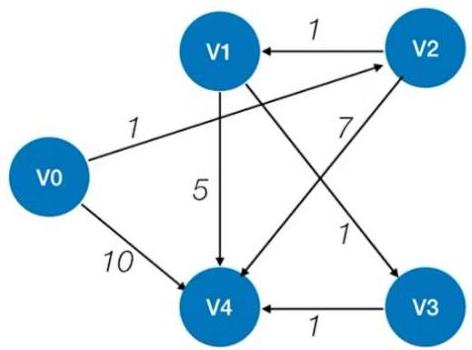
\includegraphics[width=0.6\textwidth]{images/2024/bo_d35pqfjef24c73b45bp0_4_251_309_472_350_0.jpg}
\end{center}

\begin{center}
\begin{tabular}{|c|c|c|c|c|}
\hline
\phantom{X} & \phantom{X} & \phantom{X} & \phantom{X} & \phantom{X} \\
\cline{1-5}
\phantom{X} & \phantom{X} & \phantom{X} & \phantom{X} & \phantom{X} \\
\cline{1-5}
\phantom{X} & \phantom{X} & \phantom{X} & \phantom{X} & \phantom{X} \\
\cline{1-5}
\phantom{X} & \phantom{X} & \phantom{X} & \phantom{X} & \phantom{X} \\
\cline{1-5}
\hline
\end{tabular}
\end{center}

\newpage
5. 设某通信信息由若干字母组成,字母以及其出现的次数如下表所示。 采用赫夫曼(Huffman)编码算法对上述序列编码, 给出相应的 Huffman 树, 以及每个字符的 Huffman 码。

\begin{center}
\begin{tabular}{|c|c|c|c|c|c|c|c|}
\hline
字符 & a & b & c & d & e & f & g \\
\cline{1-8}
出现频率 & 2 & 5 & 6 & 8 & 13 & 19 & 36 \\
\cline{1-8}
\hline
\end{tabular}
\end{center}

6. 对 ["Jan", "Feb", "Mar", "Apr", "May", "Jun", "Jul", "Aug", "Sep", "Oct", "Nov", "Dec"]的月份集合, 执行以下操作:

(1)构造二叉排序树,并计算查找成功的平均查找长度。

(2)对月份简写进行排序后,利用折半查找,计算查找成功的平均查找长度。

(3)构造二叉平衡树,并计算成功的平均查找长度。

\newpage

注: 所有答案必须写在答题纸上, 试卷上作答无效! 第 5 页/共 6 页

重庆邮电大学 2024 年攻读硕士学位研究生入学考试试题(回忆修订版)

\section*{四、算法设计与分析题}

1. 编写代码及思想, 判断一棵树是否为二叉排序树, 结构体已给出。

\begin{lstlisting}[language=C, basicstyle=\ttfamily]
typedef struct BiTNode {
    int data;
    struct BiTNode* lchild;
    struct BiTNode* rchild;
} BiTNode, *BiTree;
\end{lstlisting}

\newpage

2. 编写代码及思想,判断在无向图中是否存在从顶点 \(\mathrm{i}\) 到顶点 \(\mathrm{j}\) 的长度为 \(\mathrm{k}\) 的路径 (使用邻接表表示图)。

\newpage

3. 编写代码及思想, 计算二叉树的繁荣度 (即每一层的结点数乘以该层的层数)。

\newpage

\chapter{2025}
\section*{一、程序阅读题}

1. 求以下代码的时间复杂度，并分析原因。

\begin{lstlisting}[language=C, basicstyle=\ttfamily]
void move(char a, char b, int n)
{
    printf("将第%d 个盘子从%c 移动到%c\n", n, a, b);
}

void F(int n, char a, char b, char c)
{
    if(n == 1)
        move(a, c, n);
    else
    {
        F(n-1, a, c, b);
        move(a, c, n);
        F(n-1, b, a, c);
    }
}
\end{lstlisting}

2. 下列代码交换双向链表中结点和结点的前驱。请填写完整代码。双向链表存储结构及功能函数如下：

\begin{lstlisting}[language=C, basicstyle=\ttfamily]
struct DLinkNode
{
    ElementType data;
    struct DLinkNode *prior;  // Front pointer
    struct DLinkNode *next;   // Rear pointer
};

void SwapWithPrevious(DLinkNode *p)
{
    DLinkNode *q = p->prior;
    ______①______;
    p->next = q;
    // 原回忆版中②在 q->prior=p 的后面,此处交换两者顺序
    ______②______;
    q->prior = p;
    p->prior->next = p;
    q->next->prior = q;
}
\end{lstlisting}

\newpage

3. 下列代码实现循环单链表队列的出队入队，请填写完整代码。队列的链式存储类型可以描述为：

\begin{lstlisting}[language=C, basicstyle=\ttfamily]
typedef struct LinkNode
{
    ElemType data;
    struct LinkNode *next;
} LinkNode;

typedef struct
{
    LinkNode *rear;
} LinkQueue;
\end{lstlisting}

入队出队操作函数如下：

\begin{lstlisting}[language=C, basicstyle=\ttfamily]
void EnQueue(LinkQueue *Q, LinkNode *p)
{
    if(Q->rear == NULL)
    {
        Q->rear = p;
        p->next = p;
    }
    else
    {
        ______①______;
        Q->rear->next = p;
        Q->rear = p;
    }
}

LinkNode* DeQueue(LinkQueue *Q)
{
    LinkNode *p;
    if(Q->rear == NULL)
        return NULL;
    p = Q->rear->next;
    if(Q->rear == p)
        ______②______;
    else
        Q->rear->next = p->next;
    return p;
}
\end{lstlisting}

4. 下列代码实现带头结点的单链表的简单选择排序，请填写完整代码。单链表存储结构如下：

\begin{lstlisting}[language=C, basicstyle=\ttfamily]
typedef struct LNode
{
    ElemType data;
    struct LNode *next;
} LNode, *LinkList;
\end{lstlisting}

选择排序功能函数如下：

\begin{lstlisting}[language=C, basicstyle=\ttfamily]
void SelectionSort(LinkList &L)
{
    LNode *p, *q, *min;
    ______①______;

    while(p != NULL)
    {
        min = p;
        q = p->next;

        while(q != NULL)
        {
            if(q->data < min->data)
                min = q;
            q = q->next;
        }

        if(______②______)
        {
            ElemType temp = p->data;
            p->data = min->data;
            min->data = temp;
        }
        ______③______;
    }
}
\end{lstlisting}

\section*{二、填空题}

5. 分析这段代码在给定输入 a[] = \{5,4,3,2,1\} 的时间复杂度为\_\_\_\_\_\_\_\_\_\_。

\begin{lstlisting}[language=C, basicstyle=\ttfamily]
void F(int a[], int i, int n)
{
    if(i >= n-1)
        return;
    // 不是冒泡排序,若要修改,则修改成注释循环部分
    // for(int j=0; j<n-1-i; j++)
    for(int j=i; j<n-1; j++)
    {
        if(a[j] > a[j+1])
        {
            int temp = a[j];
            a[j] = a[j+1];
            a[j+1] = temp;
        }
    }
    F(a, i+1, n);
}
\end{lstlisting}

6. 元素 1,1,2,3,4 依次入栈，以 4 为开头的出栈序列有\_\_\_\_\_\_\_\_\_\_个。

7. 已知数组 \(A_{9\times 3\times 5\times 8}\)，其中 A[0][0][0][0] 的地址为 100，每一个整数占 4B，则 A[2][1][4][7] 的地址为\_\_\_\_\_\_\_\_\_\_。

8. 哈夫曼树有 199 个结点，则叶子结点有\_\_\_\_\_\_\_\_\_\_个。

9. 对于后缀表达式 1 2 4 2 / + 5 * -，经过运算后的值为\_\_\_\_\_\_\_\_\_\_。

10. 森林 F 有 15 条边，25 个结点，则森林中一共有\_\_\_\_\_\_\_\_\_\_棵树。

11. 设广义表 L = ((a,b),(c,d))，求 getHead(getTail(L)) = \_\_\_\_\_\_\_\_\_\_。

12. 利用 KMP 算法，求 abcaaba 的 next 数组\_\_\_\_\_\_\_\_\_\_。

13. 在一棵度为 4 的树 T 中，若有 20 个度为 4 的结点，10 个度为 3 的结点，1 个度为 2 的结点，10 个度为 1 的结点，则树中叶节点的个数为\_\_\_\_\_\_\_\_\_\_。

14. 如图所示，有一个小根堆，当插入后，小根堆经过调整后为\_\_\_\_\_\_\_\_\_\_。

\begin{figure}[htbp]
    \centering
    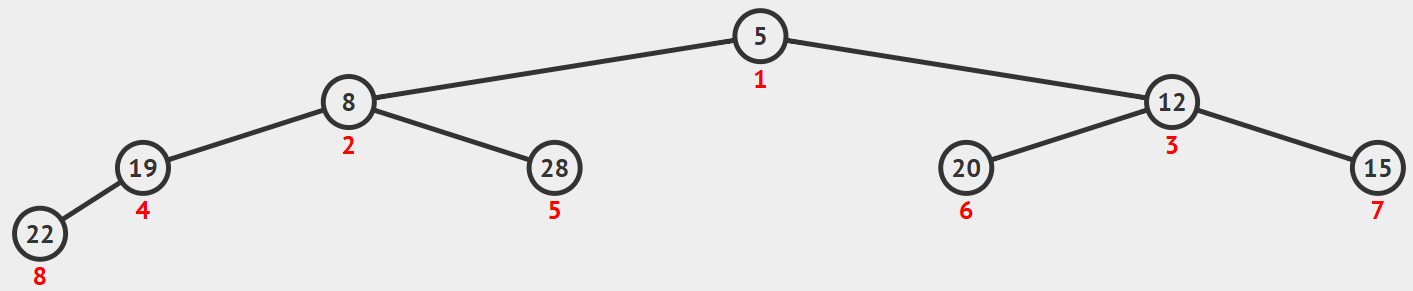
\includegraphics[width=0.3\textwidth]{images/2025/blank_14.png}
    \caption*{图1 14题图}
\end{figure}

\section*{三、综合应用题}

15. 已知一棵二叉查找树/二叉排序树(BST)的先序遍历序列为 23,15,12,18,56,29,34,71。

(1) 请画出此二叉树的形态；

(2) 请给出这棵树的后序遍历序列；

(3) 画出此二叉树的中序线索二叉树；

(4) 画出与此二叉树对应的森林。

\vspace{10em}

16. 设散列表为 HT[0...12]，即表的大小为 m=13。现采用双散列法解决冲突。散列函数和再散列函数分别为：

\[
H_{0}(key) = key \bmod 13
\]

\[
H_{i} = (H_{i-1} + (\mathrm{reverse}(key) + 1) \bmod 11 + 1) \bmod 13
\]

其中 reverse(x) 是将 x 逆置，如：reverse(789)=987。

(1) 若输入的关键码为 2,8,31,20,70,59,25,28，请画出插入这 8 个关键码后得到的散列表。

(2) 计算查找成功的平均查找长度 ASL。

\vspace{10em}

\newpage

17. 给定字符 a 到 g，它们的权值分别如下：

a:5, b:9, c:12, d:13, e:16, f:45, g:50

(1) 请根据给定的字符及其对应的权值，使用哈夫曼编码算法构建一棵哈夫曼树。要求在每次合并两个结点时，确保左结点的权值小于等于右结点的权值。

(2) 根据哈夫曼树的结构，写出每个字符的哈夫曼编码，要求左结点为 0，右结点为 1，填出下表中的对应编码。

\begin{figure}[htbp]
    \centering
    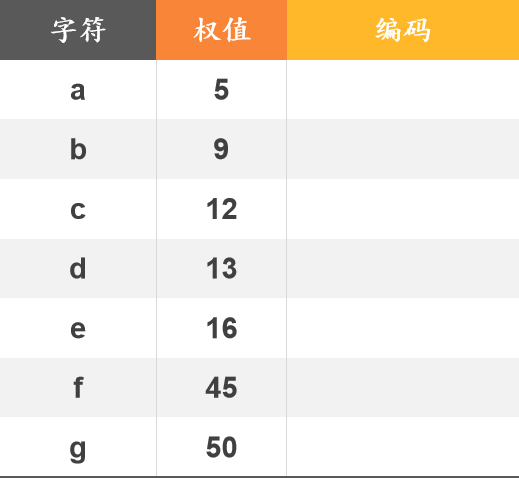
\includegraphics[width=0.3\textwidth]{images/2025/comprehensive_17.png}
    \caption*{图2 17题图}
\end{figure}

18. 已知有序数组为 [7,15,23,35,41,53,62,70,81,94]，对该数组进行二分查找，回答下列问题：

(1) 画出二叉查找树；

(2) 查找 53 需要找哪些元素；

(3) 查找 90 需要找哪些元素；

(4) 计算查找成功和查找失败的平均查找长度。

\vspace{10em}

\newpage

19. 已知带权的完全无向图 G，回答以下问题：

(1) 从 A 开始，分别写出图 G 的广度优先搜索(BFS)和深度优先搜索(DFS)序列。如果在遍历过程中有多个相同权值的路径，优先选择字母顺序较小的结点；

(2) 使用 Prim 算法从结点 A 开始构建最小生成树。如果在选择路径时存在多个相同权值的路径，优先选择字母顺序较小的结点；

(3) 使用 Kruskal 算法构建最小生成树。如果在选择路径时存在多个相同权值的路径，优先选择字母顺序较小的结点。

\begin{figure}[htbp]
    \centering
    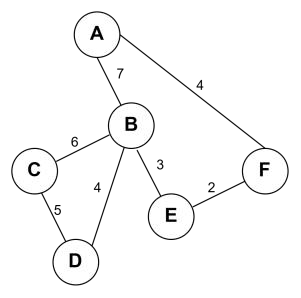
\includegraphics[width=0.3\textwidth]{images/2025/comprehensive_19.png}
    \caption*{图3 19题图}
\end{figure}

20. 给定一个 AOE 网，请回答以下问题：

(1) 计算每个事件的最早发生时间(\(ve\))和最晚发生时间(\(vl\))；

(2) 计算每个活动的最早开始时间(\(e\))和最迟开始时间(\(l\))；

(3) 确定关键路径。

\begin{figure}[htbp]
    \centering
    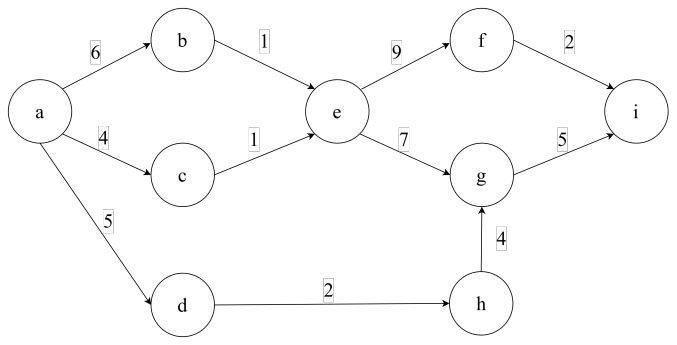
\includegraphics[width=0.3\textwidth]{images/2025/comprehensive_20.png}
    \caption*{图4 20题图}
\end{figure}

\newpage

\section*{四、算法设计与分析题}

21. 给定一个单链表，找到倒数第 k 个元素。如果找到该元素，打印该元素的值并返回 1，否则返回 0。

(1) 描述算法的基本设计思想；

(2) 根据设计思想，采用 C 语言描述算法。

结点定义如下：

\begin{lstlisting}[language=C, basicstyle=\ttfamily]
typedef struct node
{
    int data;
    struct node *next;
} LNode, *LinkList;
\end{lstlisting}

\vspace{15em}

\newpage

22. 给定一棵二叉树，输出从根结点到叶子结点的最长路径，打印路径的结点值，并输出该路径的长度。

(1) 描述算法的基本设计思想；

(2) 根据设计思想，采用 C 语言描述算法。

二叉树的链式存储结构描述如下：

\begin{lstlisting}[language=C, basicstyle=\ttfamily]
typedef struct BiTNode {
    ElemType data;
    struct BiTNode *lchild, *rchild;
} BiTNode, *BiTree;
\end{lstlisting}

\vspace{15em}

\newpage

23. 给定一个邻接表表示的连通图，输出从顶点 \(u\) 到顶点 \(v\) 并经过顶点 \(k\) 的一条路径。如果不存在这样的路径，输出 -1。

(1) 描述算法的基本设计思想；

(2) 根据设计思想，采用 C 语言描述算法。

图的存储结构描述如下：

\begin{lstlisting}[language=C, basicstyle=\ttfamily]
#define MaxVertexNum 100
typedef char InfoType;   // 附加信息类型
typedef int VertexType;  // 顶点数据类型

typedef struct ArcNode {  // 边表结点
    int adjvex;           // 该弧所指向的顶点位置
    struct ArcNode *next; // 下个结点
    // InfoType info;     // 当前结点（弧）的信息
} ArcNode;

typedef struct VNode {        // 顶点表结点
    VertexType data;          // 顶点信息
    ArcNode *firstarc;        // 指向第一条依附该顶点的弧的指针
} VNode, AdjList[MaxVertexNum];

typedef struct {              // 图
    AdjList vertices;         // 邻接表
    int vexnum, arcnum;       // 图的当前顶点数,图的边数/弧数
} ALGraph;
\end{lstlisting}

\newpage

\chapter{2026}
\section*{一、程序阅读题}

1. 下面代码是关于深度优先生成树，请填写完整代码。图的邻接表存储结构及功能函数如下：

\begin{lstlisting}[language=C, basicstyle=\ttfamily]
typedef int VertexType; // 顶点数据类型

typedef struct ArcNode {  // 边表结点
    int adjvex;           // 该弧所指向的顶点位置
    struct ArcNode *nextarc; // 下个结点
} ArcNode;

typedef struct VNode {        // 顶点表结点
    VertexType data;          // 顶点信息
    ArcNode *firstarc;        // 指向第一条依附该顶点的弧的指针
} VNode;

typedef struct {              // 图
    VNode vertices[MaxVertexNum]; // 邻接表
    int vexnum, arcnum;       // 图的当前顶点数,图的边数/弧数
} ALGraph;

void DFS_Tree(ALGraph G)
{
    for(int i=0; i<G.vexnum; i++)
        visited[i] = false;
    for(int i=0; i<G.vexnum; i++)
        if(!visited[i])
            DFSTree(G, i);
}

void DFSTree(ALGraph G, int v)
{
    visited[v] = true;
    ArcNode *p = _____(1)_____;
    while(p != NULL)
    {
        if(!visited[p->adjvex])
        {
            printf("Tree edge:\%d \%d\n", v, p->adjvex);
            _____(2)_____;
        }
        p = p->nextarc;
    }
}
\end{lstlisting}

2. 给定一个共享栈，栈大小为 m，栈 1 的初始栈顶指针 top[0] 值初始指向 -1，栈 2 的初始栈顶指针 top[1] 值初始指向 m，请填写完整代码。共享栈存储类型可以描述为（题目中未给出该部分存储结构）：

\begin{lstlisting}[language=C, basicstyle=\ttfamily]
typedef struct
{
    int data[MaxSize];
    int top[2];  // 栈顶指针
    int bot[2];  // 栈尾指针
} TwStack;
\end{lstlisting}

初始化、入队和出队操作函数如下：

\begin{lstlisting}[language=C, basicstyle=\ttfamily]
void InitStack(TwStack &S)
{
    S.bot[0] = -1;
    S.bot[1] = m;
    S.top[0] = -1;
    S.top[1] = m;
}

bool Push(TwStack &S, int i, int x)
{
    if(_____(1)_____)
        return false;
    if(i == 0)
        S.data[_____(2)_____] = x;
    else if(i == 1)
        S.data[_____(3)_____] = x;
    return true;
}

bool Pop(TwStack &S, int i, int &x)
{
    if(S.top[i] == S.bot[i])
        return false;
    if(i == 0)
        x = S.data[_____(4)_____];
    else if(i == 1)
        x = S.data[_____(5)_____];
    return true;
}
\end{lstlisting}

\newpage

3. 假设有两个带头结点线性表 A 和 B，它们的元素都是依值递增有序排列，并且分别表示两个集合，现要求另辟空间构成一个线性表 C，其元素为 A 和 B 中元素的交集，且表 C 中的元素也依值递增有序排列。借助线性表 A 空间存放线性表 C，请填写完整代码。

\begin{lstlisting}[language=C, basicstyle=\ttfamily]
Status merge_list(LinkList &A, LinkList &B)
{
    LNode *pa = A->next;
    LNode *pb = B->next;
    LNode *pc = A;
    LNode *temp;

    while(_____(1)_____)
    {
        if(pa->data == pb->data)
        {
            _____(2)_____;
            pc = pa;
            pa = pa->next;
            temp = pb;
            pb = pb->next;
            free(temp);
        }
        else if(pa->data < pb->data)
        {
            temp = pa;
            pa = pa->next;
            free(temp);
        }
        else
        {
            temp = pb;
            pb = pb->next;
            free(temp);
        }
    }

    while(pb)
    {
        temp = pb;
        pb = pb->next;
        free(temp);
    }

    while(pa)
    {
        temp = pa;
        pa = pa->next;
        free(temp);
    }
    _____(3)_____;
    free(B);
    return OK;
}
\end{lstlisting}

4. 分析下列程序的输出结果，并给出算法的时间复杂度，其中 n 为 8。

\begin{lstlisting}[language=C, basicstyle=\ttfamily]
int a[] = {23, 33, 16, 79, 34, 79, 29, 86};

void riddle1(int n)
{
    if(n == 1)
        return;
    riddle1(n-1);
    if(a[n-1] < a[n-2])
        printf("%d ", a[n-1]);
    else
        printf("%d ", a[n-2]);
}

int riddle2(int n)  // 两函数不确定是哪个
{
    if(n == 1)
        return a[0];
    int p = riddle2(n-1);
    if(p < a[n])
        return p;
    else
        return a[n];
}
\end{lstlisting}

\newpage

5. 下面的代码是判断一个二叉树是否为平衡二叉树，若是平衡二叉树通过参数 depth 返回树的深度，并返回 true；若不是平衡二叉树，则返回 false，此时 depth 的值无意义。请填写完整代码。

二叉树的链式存储结构描述如下：

\begin{lstlisting}[language=C, basicstyle=\ttfamily]
typedef struct BiTNode {
    ElemType data;
    struct BiTNode *lchild, *rchild;
} BiTNode, *BiTree;
\end{lstlisting}

判断平衡二叉树函数如下：

\begin{lstlisting}[language=C, basicstyle=\ttfamily]
bool isBalanced(BiTree T, int &depth)
{
    if(T == NULL)
    {
        depth = 0;
        return true;
    }
    int deepleft, deepright;

    if(_____(1)_____)
    {
        int dif = deepleft - deepright;
        if(_____(2)_____)
        {
            depth = (deepleft > deepright ? deepleft : deepright) + 1;
            return true;
        }
    }
    return false;
}
\end{lstlisting}

\section*{二、填空题}

6. 已知 a=2, b=3, c=4, d=5，求出后缀表达式 abc*+d- 的计算值为\_\_\_\_\_\_\_\_\_\_。

7. 若用一个大小为 5 的数组来实现循环队列，且当前 front 和 rear 的值分别是 0 和 3，从队列中进队 1 次，出队 2 次后，front 和 rear 的值分别是\_\_\_\_\_\_\_\_\_\_。

8. 二维数组 A 按行优先存储，每个元素占 1 个空间，若 A[0][0] 的地址为 100，A[3][3] 地址为 220，则 A[5][5] 的地址为\_\_\_\_\_\_\_\_\_\_。

9. 栈按 1 到 n 依次进栈，出队序列为 \(T_{1},T_{2},\dots,T_{n}\)，若 \(T_{1}\) 为 n，则第 i 个出队的元素是\_\_\_\_\_\_\_\_\_\_。

10. 含有 n 个顶点的强连通图，边数至少为\_\_\_\_\_\_\_\_\_\_。

11. 含有 n 个结点的二叉树，在二叉链表中的空指针个数为\_\_\_\_\_\_\_\_\_\_。

12. 若长度为 n 的线性表采用链式存储结构，在其第 i 个位置插入一个元素的时间复杂度为\_\_\_\_\_\_\_\_\_\_。

13. 含 125 个元素的数组，折半查找成功的最多比较次数为\_\_\_\_\_\_\_\_\_\_。

14. 已知广义表 A = (a,b,(c,d),(e,(f,g)))，则 Head(Tail(Head(Tail(Tail(A))))) 的值为\_\_\_\_\_\_\_\_\_\_。

15. 无原题。下面是 AI 生成的类似的题目：给定一个大根堆 [9,6,8,3,4,5,7]，当插入元素 10 后，大根堆经过调整后，需要的比较次数为\_\_\_\_\_\_\_\_\_\_。

\begin{figure}[htbp]
    \centering
    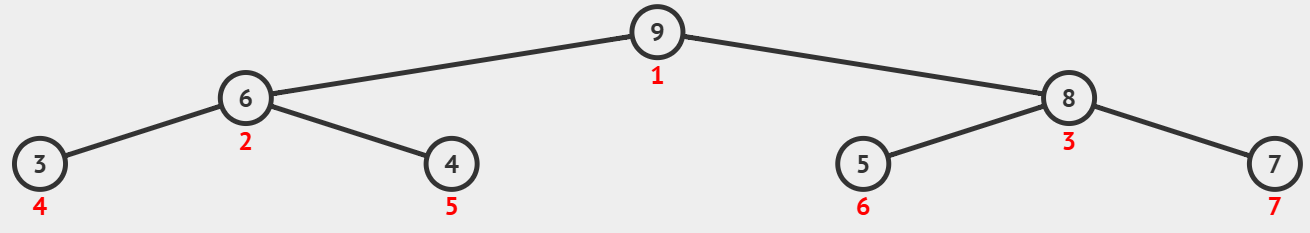
\includegraphics[width=0.3\textwidth]{images/2026/blank_15.png}
    \caption*{图1 15题图}
\end{figure}

\section*{三、综合应用题}
（回忆版综合应用题的序列、图不一定与考试一致，综合题顺序不一定一致）

16. 已知某二叉树的先序序列为 ABCDEFG，中序序列为 BADCFEG。

(1) 画出该二叉树，并给出该二叉树的后序序列；

(2) 画出该二叉树的三叉链表结构；

(3) 画出该二叉树对应的树或森林。

\vspace{10em}

17. 有一个散列表（也称哈希表）的散列函数为 H(key) = key \% 13，将关键字序列 19,14,23,1,68,20,84,27,55,11,10,79 按顺序插入空的哈希表：

(1) 若采用线性探测法处理冲突，请画出插入完成的哈希表，并求等概率下查找成功和查找失败时的平均查找长度，注意哈希表为 HT[0,\dots,15]，表长为 16。

(2) 若采用链地址法处理冲突，请画出插入完成的哈希表，并求等概率情况下查找成功和查找失败时的平均查找长度。

\vspace{10em}

\newpage

18. 给定一个整数序列 \{14,4,39,28,16,2,10,78\}

(1) 画出依次插入二叉排序树的最终形态；

(2) 计算查找成功的平均查找长度；

(3) 若一开始插入时进行平衡调整，给出最终的平衡二叉树的形态。

\vspace{10em}

19. 给定一个有向图，利用 Dijkstra 算法寻找从 V1 作为源点的最短路径。

\begin{figure}[htbp]
    \centering
    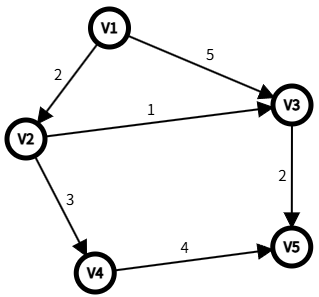
\includegraphics[width=0.3\textwidth]{images/2026/comprehensive_19_1.png}
    \caption*{图2 19题图1}
\end{figure}
\begin{figure}[htbp]
    \centering
    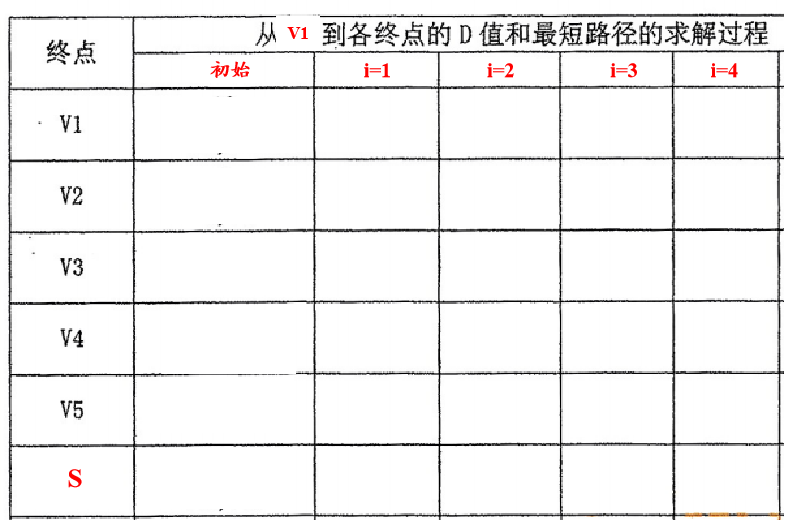
\includegraphics[width=0.3\textwidth]{images/2026/comprehensive_19_2.png}
    \caption*{图3 19题图2}
\end{figure}

\newpage

20. 给定一个 AOE 网，完成表格，要求给出计算过程，并给出关键路径。

\begin{figure}[htbp]
    \centering
    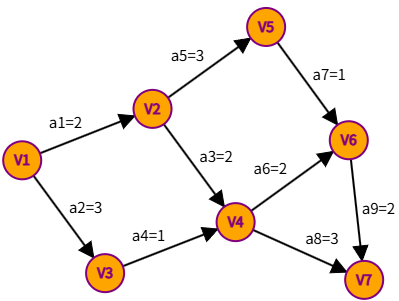
\includegraphics[width=0.3\textwidth]{images/2026/comprehensive_20.png}
    \caption*{图4 20题图}
\end{figure}

\begin{center}
\begin{tabular}{|c|c|c|c|c|c|c|c|}
\hline
事件 & V1 & V2 & V3 & V4 & V5 & V6 & V7 \\
\hline
最早发生时间 & \phantom{X} & \phantom{X} & \phantom{X} & \phantom{X} & \phantom{X} & \phantom{X} & \phantom{X} \\
\hline
最迟发生时间 & \phantom{X} & \phantom{X} & \phantom{X} & \phantom{X} & \phantom{X} & \phantom{X} & \phantom{X} \\
\hline
\end{tabular}
\end{center}

\vspace{2em}

\begin{center}
\begin{tabular}{|c|c|c|c|c|c|c|c|c|c|}
\hline
活动 & a1 & a2 & a3 & a4 & a5 & a6 & a7 & a8 & a9 \\
\hline
最早开始时间 & \phantom{X} & \phantom{X} & \phantom{X} & \phantom{X} & \phantom{X} & \phantom{X} & \phantom{X} & \phantom{X} & \phantom{X} \\
\hline
最迟开始时间 & \phantom{X} & \phantom{X} & \phantom{X} & \phantom{X} & \phantom{X} & \phantom{X} & \phantom{X} & \phantom{X} & \phantom{X} \\
\hline
\end{tabular}
\end{center}

\vspace{10em}

\newpage

21. 已知字母 a\(\sim\)g 的频率如下表所示。

(1) 采用赫夫曼（Huffman）编码算法对上述序列编码，给出相应的 Huffman 树，要求同一结点的左根大于右根；

(2) 对每个字母给出对应的编码，左 0 右 1，完成下表。

\begin{center}
\begin{tabular}{|c|c|c|c|c|c|c|c|}
\hline
字符 & a & b & c & d & e & f & g \\
\hline
出现频率 & 5 & 9 & 12 & 13 & 16 & 45 & 6 \\
\hline
编码 & \phantom{X} & \phantom{X} & \phantom{X} & \phantom{X} & \phantom{X} & \phantom{X} & \phantom{X} \\
\hline
\end{tabular}
\end{center}

\vspace{10em}

22. 给定有序序列 \{2,7,8,10,24,25,28,31,33,39,41\}

(1) 画出折半查找判定树；

(2) 查找元素 28 需要依次比较哪些元素；

(3) 在相等查找概率情况下，计算查找成功的平均查找长度。

\vspace{10em}

\newpage

23. 已知整数序列 \{46,79,56,38,40,84,29,10,15,37\}

(1) 将该序列建立初始小根堆，并写出最终形态的小根堆；

(2) 使用二路归并排序对原序列进行升序排序，写出每趟归并后的结果；

(3) 以第一个元素 46 作为 pivot，对原序列进行一趟快速排序（第一趟分区后的结果）。

\vspace{10em}

\newpage

\section*{四、算法分析题}

24. 编号为 1 到 n 的 n 个人围成一个圈，现从编号为 s 的人开始按顺时针方向报数（从 1 开始报），报到 m 的人离开圈子。然后他的下一个人开始重新从 1 开始报数，重复此过程，直到所有人都离开为止。

举例：n=8, s=1, m=4，离开次序为 4,8,5,2,1,3,7,6

要求使用链表实现，使用 C 语言完成下列函数，关键之处给出注释。

\begin{lstlisting}[language=C, basicstyle=\ttfamily]
void joseph(int n, int s, int m)
\end{lstlisting}

\vspace{15em}

\newpage

25. 设一棵二叉树中的各结点的值互不相同，其先序遍历序列和中序遍历序列分别存在两个一维数组 A[1,\dots,n] 和 B[1,\dots,n] 中，试编写算法建立该二叉树的二叉链表，使用 C 语言，关键之处给出注释。

二叉树的链式存储结构描述如下：

\begin{lstlisting}[language=C, basicstyle=\ttfamily]
typedef struct BiTNode {
    ElemType data;
    struct BiTNode *lchild, *rchild;
} BiTNode, *BiTree;
\end{lstlisting}

\vspace{15em}

\newpage

26. 给一个由邻接表存储的有向图，给定一个序列 \(\{V_{1}, V_{2}, \dots, V_{n}\}\) 判断该序列是否为该图的一个拓扑排序序列，若是返回 1，反之返回 0，请给出 C 语言的算法代码，关键之处给出注释。

图的存储结构描述如下：

\begin{lstlisting}[language=C, basicstyle=\ttfamily]
typedef int VertexType; // 顶点数据类型

typedef struct ArcNode {  // 边表结点
    int adjvex;           // 该弧所指向的顶点位置
    struct ArcNode *nextarc; // 下个结点
} ArcNode;

typedef struct VNode {        // 顶点表结点
    VertexType data;          // 顶点信息
    ArcNode *firstarc;        // 指向第一条依附该顶点的弧的指针
} VNode;

typedef struct {              // 图
    VNode vertices[MaxVertexNum]; // 邻接表
    int vexnum, arcnum;       // 图的当前顶点数,图的边数/弧数
} ALGraph;
\end{lstlisting}

\newpage

\printbibliography
\end{document}
